%%%%%%%%%%%%%%%%%%%%%%%%%%%%%%%%%%%%%%%%%
% Masters/Doctoral Thesis 
% LaTeX Template
% Version 2.5 (27/8/17)
%
% This template was downloaded from:
% http://www.LaTeXTemplates.com
%
% Version 2.x major modifications by:
% Vel (vel@latextemplates.com)
%
% This template is based on a template by:
% Steve Gunn (http://users.ecs.soton.ac.uk/srg/softwaretools/document/templates/)
% Sunil Patel (http://www.sunilpatel.co.uk/thesis-template/)
%
% Template license:
% CC BY-NC-SA 3.0 (http://creativecommons.org/licenses/by-nc-sa/3.0/)
%
%%%%%%%%%%%%%%%%%%%%%%%%%%%%%%%%%%%%%%%%%

%----------------------------------------------------------------------------------------
%	PACKAGES AND OTHER DOCUMENT CONFIGURATIONS
%----------------------------------------------------------------------------------------

\documentclass[
11pt, % The default document font size, options: 10pt, 11pt, 12pt
%oneside, % Two side (alternating margins) for binding by default, uncomment to switch to one side
spanish, % ngerman for German
singlespacing, % Single line spacing, alternatives: onehalfspacing or doublespacing
%draft, % Uncomment to enable draft mode (no pictures, no links, overfull hboxes indicated)
%nolistspacing, % If the document is onehalfspacing or doublespacing, uncomment this to set spacing in lists to single
%liststotoc, % Uncomment to add the list of figures/tables/etc to the table of contents
%toctotoc, % Uncomment to add the main table of contents to the table of contents
%parskip, % Uncomment to add space between paragraphs
%nohyperref, % Uncomment to not load the hyperref package
headsepline, % Uncomment to get a line under the header
% chapterinoneline, % Uncomment to place the chapter title next to the number on one line
% consistentlayout, % Uncomment to change the layout of the declaration, abstract and acknowledgements pages to \textit{match} the default layout
]{MastersDoctoralThesis} % The class file specifying the document structure

\usepackage[utf8]{inputenc} % Required for inputting international characters
\usepackage[T1]{fontenc} % Output font encoding for international characters
\usepackage{comment}
\usepackage{mathpazo} % Use the Palatino font by default
\usepackage{graphicx}
\usepackage[backend=bibtex,bibencoding=ascii,style=numeric,natbib=true]{biblatex} % Use the bibtex backend with the authoryear citation style (which resembles APA)

\addbibresource{example.bib} % The filename of the bibliography

\usepackage[autostyle=true]{csquotes} % Required to generate language-dependent quotes in the bibliography
\usepackage{float}
% \usepackage{tabu}
\usepackage{booktabs}
% \usepackage[table,xcdraw]{xcolor}

%----------------------------------------------------------------------------------------
%	MARGIN SETTINGS
%----------------------------------------------------------------------------------------

\geometry{
	paper=a4paper, % Change to letterpaper for US letter
	outer=2.5cm, % Inner margin
	inner=3.8cm, % Outer margin
	bindingoffset=.5cm, % Binding offset
	top=1.5cm, % Top margin
	bottom=1.5cm, % Bottom margin
	%showframe, % Uncomment to show how the type block is set on the page
}

%----------------------------------------------------------------------------------------
%	THESIS INFORMATION
%----------------------------------------------------------------------------------------

\thesistitle{Administración de un muxponder a través de Redes Definidas Por Software} % Your thesis title, this is used in the title and abstract, print it elsewhere with \ttitle
\supervisor{Ing. Hugo \textsc{Carrer}} % Your supervisor's name, this is used in the title page, print it elsewhere with \supname
\examiner{Matthew \textsc{Aguerreberry}} % Your examiner's name, this is not currently used anywhere in the template, print it elsewhere with \examname
% \degree{Doctor of Philosophy} % Your degree name, this is used in the title page and abstract, print it elsewhere with \degreename
\authorA{Matias \textsc{Kleiner}}
\matriculaA{37590431}
\emailA{\texttt{kleiner.matias@gmail.com}}
\authorB{ " }
\matriculaB{ " }
\emailB{ " }
% Your name, this is used in the title page and abstract, print it elsewhere with \authorname
% \addresses{} % Your address, this is not currently used anywhere in the template, print it elsewhere with \addressname

% \subject{Biological Sciences} % Your subject area, this is not currently used anywhere in the template, print it elsewhere with \subjectname
\keywords{Software Defined Networking (SDN), Administracion, Open Networking Operating System (ONOS)} % Keywords for your thesis, this is not currently used anywhere in the template, print it elsewhere with \keywordnames
\university{Universidad Nacional de Córdoba} % Your university's name and URL, this is used in the title page and abstract, print it elsewhere with \univname
% \department{Facultad de Ciencias Exactas Físicas y Naturales} % Your department's name and URL, this is used in the title page and abstract, print it elsewhere with \deptname
% \group{\href{http://researchgroup.university.com}{Research Group Name}} % Your research group's name and URL, this is used in the title page, print it elsewhere with \groupname
\faculty{Facultad de Ciencias Exactas Físicas y Naturales} % Your faculty's name and URL, this is used in the title page and abstract, print it elsewhere with \facname

\AtBeginDocument{
\hypersetup{pdftitle=\ttitle} % Set the PDF's title to your title
\hypersetup{pdfauthor=\authornameA} % Set the PDF's author to your name
\hypersetup{pdfkeywords=\keywordnames} % Set the PDF's keywords to your keywords
}

\begin{document}

\frontmatter % Use roman page numbering style (i, ii, iii, iv...) for the pre-content pages

\pagestyle{plain} % Default to the plain heading style until the thesis style is called for the body content

%----------------------------------------------------------------------------------------
%	TITLE PAGE
%----------------------------------------------------------------------------------------

\begin{titlepage}
	\begin{center}
				
		\resizebox{1\textwidth}{!}{
\includegraphics{Figures/logo-unc-fcefyn.png}}%
				
		\vspace*{.06\textheight}
		{\scshape\LARGE \univname\par}\vspace{0.5cm} % University name
		{\scshape\LARGE \facname\par}\vspace{1.5cm}
		\textsc{\Large Proyecto Integrador}\\[0.5cm] % Thesis type
		\textsc{\Large Ingeniería en Computación}\\[0.5cm]
				
		\HRule \\[0.4cm] % Horizontal line
		{\huge \bfseries \ttitle\par}\vspace{0.4cm} % Thesis title
		\HRule \\[1.5cm] % Horizontal line
				 
		\begin{minipage}[t]{0.5\textwidth}
			\begin{flushleft} \large
				\emph{Autor:}\\
				\authornameA \\ % Author name - remove the \href bracket to remove the link
				\matriculanameA \\
				\emailnameA
				\\~\\
				
			\end{flushleft}
		\end{minipage}
		\begin{minipage}[t]{0.4\textwidth}
			\begin{flushright} \large
				\emph{Director:} \\
				\supname \\
				\emph{Co-director:} \\
				\examname
			\end{flushright}
		\end{minipage}\\[2cm]
				 
		\vfill
				
		% \large \textit{A thesis submitted in fulfillment of the requirements\\ for the degree of \degreename}\\[0.3cm] % University requirement text
		% \textit{in the}\\[0.4cm]
		% \groupname\\\deptname\\[2cm] % Research group name and department name
				 
		\vfill
				
		{\large {Julio 2019}}\\[4cm] % Date
		%\includegraphics{Logo} % University/department logo - uncomment to place it
				 
		\vfill
	\end{center}
\end{titlepage}

%----------------------------------------------------------------------------------------
%	DEDICATION
%----------------------------------------------------------------------------------------

\dedicatory{Para mi familia\ldots} 

% %----------------------------------------------------------------------------------------
% %	DECLARATION PAGE
% %----------------------------------------------------------------------------------------

% \begin{declaration}
% \addchaptertocentry{\authorshipname} % Add the declaration to the table of contents
% \noindent I, \authorname, declare that this thesis titled, \enquote{\ttitle} and the work presented in it are my own. I confirm that:

% \begin{itemize} 
% \item This work was done wholly or mainly while in candidature for a research degree at this University.
% \item Where any part of this thesis has previously been submitted for a degree or any other qualification at this University or any other institution, this has been clearly stated.
% \item Where I have consulted the published work of others, this is always clearly attributed.
% \item Where I have quoted from the work of others, the source is always given. With the exception of such quotations, this thesis is entirely my own work.
% \item I have acknowledged all main sources of help.
% \item Where the thesis is based on work done by myself jointly with others, I have made clear exactly what was done by others and what I have contributed myself.\\
% \end{itemize}
 
% \noindent Signed:\\
% \rule[0.5em]{25em}{0.5pt} % This prints a line for the signature
 
% \noindent Date:\\
% \rule[0.5em]{25em}{0.5pt} % This prints a line to write the date
% \end{declaration}

% \cleardoublepage

%----------------------------------------------------------------------------------------
%	QUOTATION PAGE
%----------------------------------------------------------------------------------------

% \vspace*{0.2\textheight}

% \noindent\enquote{\itshape Thanks to my solid academic training, today I can write hundreds of words on virtually any topic without possessing a shred of information, which is how I got a good job in journalism.}\bigbreak

% \hfill Dave Barry

%----------------------------------------------------------------------------------------
%	ABSTRACT PAGE
%----------------------------------------------------------------------------------------

\begin{abstract}
	\addchaptertocentry{\abstractname} % Add the abstract to the table of contents
	\begin{comment}
	Con el extraordinario incremento del tráfico de datos en Internet provocado, entre otros, por dispositivos móviles (LTE, 4G), servicios en la nube (Amazon, Netflix, iCloud, Azure, etc.) y migración de información entre centros de datos, las infraestructuras de red actuales se ven comprometidas a la hora de brindar una calidad de servicio satisfactorio. Este esquema de red resulta inadecuado para adaptarse a estos nuevos requerimientos, esto se debe principalmente a su gran complejidad, difícil escalamiento, políticas inconsistentes y falta de compatibilidad entre fabricantes de dispositivos de red.
		
	El nuevo paradigma que propone \textit{Software Defined Networking} (SDN) lo convierte en el mejor candidato para resolver estos problemas. SDN consiste, conceptualmente, en una separación del plano de control y datos en toda la infraestructura de la red. Empleando una interfaz entre ambos planos, denominada controlador, este nuevo esquema permite gestionar la red con una visión global del sistema. De esta forma, la infraestructura de la red se vuelve flexible e independiente de los servicios que se implementen sobre ella.
		
	En este proyecto integrador se busca, en primer lugar, adquirir en su totalidad los conocimientos involucrados con \textit{Software Defined Networking}. Luego, como medio de prueba se diseña e implementa una aplicación de distribución de contenido \textit{multicast} utilizando exclusivamente las funcionalidades que brinda SDN. Asimismo, se genera una interfaz de usuario para la sencilla administración de la distribución de contenido \textit{multicast}. Además, se desarrolla un ambiente de emulación de redes reales para la verificación y validación de la aplicación, con el agregado de que uno de los nodos fue implementado físicamente e integrado a la red virtual. Finalmente, se brindan distintas ideas para mejorar lo aquí implementado y posibles vías para continuar trabajando en el ámbito de las redes definidas por software.
\end{comment} 
\end{abstract}

% \textbf{Palabras Clave:} \textit{\keywordnames}

%----------------------------------------------------------------------------------------
%	ACKNOWLEDGEMENTS
%----------------------------------------------------------------------------------------
 
\begin{acknowledgements}
	
	\addchaptertocentry{\acknowledgementname} % Add the acknowledgements to the table of contents

	% 	{\normalsize padres y hermanos \par}
	Muchas gracias a mi familia, por su apoyo incondicional a lo largo de todos estos años de estudio.  
	\bigskip
			
	% 	{\normalsize Hugo y Matt \par}
	Este proyecto no hubiera sido posible sin el soporte, la confianza, la supervisión y el duro empeño de nuestros directores, Hugo Carrer y Matthew Aguerreberry.
	\bigskip
			
	% 	{\normalsize amigos \par}
	Un especial agradecimiento a mis amigos, y todas las personas que tuve el placer de conocer durante estos años de carrera.
	\bigskip
		
	% 	{\normalsize Fundación y gente que labura en la funda \par}
	Agradezco a la Fundación Fulgor y a la Fundación Tarpuy, y a todo su personal, por las oportunidades y enseñanzas compartidas.
	\bigskip
			
	% 	{\normalsize universisdad / profes de la facu \par}
	Finalmente, agradecemos a la Facultad de Ciencias Exactas Físicas y Naturales de la Universidad Nacional de Córdoba por la oportunidad de realizar esta carrera de grado.

	\vspace*{\fill}
		
\end{acknowledgements}

%----------------------------------------------------------------------------------------
%	LIST OF CONTENTS/FIGURES/TABLES PAGES
%----------------------------------------------------------------------------------------

\hypersetup{
	linkcolor=black,
	citecolor=black,
	urlcolor=black
	}

\tableofcontents % Prints the main table of contents

\listoffigures % Prints the list of figures

\listoftables % Prints the list of tables

%----------------------------------------------------------------------------------------
%	ABBREVIATIONS
%----------------------------------------------------------------------------------------

\begin{abbreviations}{ll} % Include a list of abbreviations (a table of two columns)
		
	\textbf{API} & \textbf{A}pplication \textbf{P}rogramming \textbf{I}nterface\\
	\textbf{CLI} & \textbf{C}ommand \textbf{L}ine \textbf{I}nterface\\
	\textbf{SNMP} & \textbf{S}imple \textbf{N}etwork \textbf{M}anagement \textbf{P}rotocol\\
	%\textbf{FIB} & \textbf{F}orwarding \textbf{I}nformation \textbf{B}ase\\
	\textbf{GUI} & \textbf{G}raphical \textbf{U}ser \textbf{I}nterface\\
	%\textbf{IGMP} & \textbf{I}nternet \textbf{G}roup \textbf{M}anagement \textbf{P}rotocol\\
	%\textbf{NFV} & \textbf{N}etwork \textbf{F}unction \textbf{V}irtualization\\
	%\textbf{ODL} & \textbf{O}pen\textbf{D}ay\textbf{l}ight\\
	\textbf{ONF} & \textbf{O}pen \textbf{N}etworking \textbf{F}oundation\\
	\textbf{IETF} & \textbf{I}nternet \textbf{E}ngineering \textbf{T}ask \textbf{F}orce\\
	%\textbf{ONOS} & \textbf{O}pen \textbf{N}etworking \textbf{O}perating \textbf{S}ystem\\
	%\textbf{OVS} & \textbf{O}pen \textbf{V} \textbf{S}witch\\
	%\textbf{PIM} & \textbf{P}rotocol \textbf{I}ndependent \textbf{M}ulticast\\
	%\textbf{RIB} & \textbf{R}outing \textbf{I}nformation \textbf{B}ase\\
	%\textbf{REST} & \textbf{RE}presentational \textbf{S}tate \textbf{T}ransfer\\
	\textbf{SDN} & \textbf{S}oftware \textbf{D}efined \textbf{N}etwork\\
	%\textbf{SSM} & \textbf{S}ource \textbf{S}pecific \textbf{M}ulticast\\
	\textbf{UDP} & \textbf{U}ser \textbf{D}atagram \textbf{P}rotocol\\
	\textbf{TCP} & \textbf{T}ransmission \textbf{C}ontrol \textbf{P}rotocol\\
	\textbf{MIB} & \textbf{M}anagement \textbf{I}nformation \textbf{B}ase\\
	\textbf{TLS} & \textbf{T}ransport \textbf{L}ayer \textbf{S}ecurity\\
	\textbf{SSH} & \textbf{S}ecure \textbf{SH}ell\\
	\textbf{OTN} & \textbf{O}ptical \textbf{T}ransport \textbf{N}etwork\\
	\textbf{OTU} & \textbf{O}ptical \textbf{T}ransport \textbf{U}nit\\
	\textbf{ITU} & \textbf{I}nternational \textbf{T}elecommunication \textbf{U}nion\\
	\textbf{RFC} & \textbf{R}equest \textbf{F}or \textbf{C}omments\\
	\textbf{RPC} & \textbf{R}emote \textbf{P}rocedure \textbf{C}all\\
	\textbf{XML} & E\textbf{X}tensible \textbf{M}arkup \textbf{L}anguage\\
	\textbf{YANG} & \textbf{Y}et \textbf{A}nother \textbf{N}ext \textbf{G}eneration\\
	\textbf{NETCONF} & \textbf{NET}work \textbf{CONF}iguration Protocol\\
	\textbf{IANA} & \textbf{I}nternet \textbf{A}ssigned \textbf{N}umbers \textbf{A}uthority\\
	\textbf{FEC} & \textbf{F}orward \textbf{E}rror \textbf{C}orrection\\
	\textbf{FPGA} & \textbf{F}ield \textbf{P}rogrammable \textbf{G}ate \textbf{A}rray\\
	\textbf{ONOS} & \textbf{O}pen \textbf{N}etwork \textbf{O}perating \textbf{S}ystem\\
	\textbf{REST} & \textbf{RE}presentational \textbf{S}tate \textbf{T}ransfer\\
	\textbf{BSD} & \textbf{B}erkeley \textbf{S}oftware \textbf{D}istribution\\
	\textbf{MIT} & \textbf{M}assachusetts \textbf{I}nstitute \textbf{T}echnology\\
	
	%\textbf{VNF} & \textbf{V}irtual \textbf{N}etwork \textbf{F}unction\\
				 
\end{abbreviations}
%----------------------------------------------------------------------------------------
%	THESIS CONTENT - CHAPTERS
%----------------------------------------------------------------------------------------

\mainmatter % Begin numeric (1,2,3...) page numbering

\pagestyle{thesis} % Return the page headers back to the "thesis" style

% Include the chapters of the thesis as separate files from the Chapters folder
% Uncomment the lines as you write the chapters

 % Chapter Template

\chapter{Introducción} % Main chapter title

\label{Chapter1} % Change X to a consecutive number; for referencing this chapter elsewhere, use \ref{ChapterX}

Las redes de telecomunicaciones crecen a medida que surgen nuevas tecnologías (redes inalámbricas \textit{4G} y \textit{5G}, \textit{WiMax}, \textit{LTE}, etc), seguido de la demanda en alza del ancho de banda por parte de los usuarios, requiriendo así cada vez mayor velocidad y mejor calidad de servicio. De esta forma, los operadores de red se ven obligados a aumentar la cantidad de dispositivos para satisfacer las necesidades de los usuarios, lo que constituye un desafío y un problema para los administradores de red, donde serán necesarios mecanismos de configuración que se adapten a las nuevas necesidades. 

Así, el paradigma actual de implementación de redes resulta difícil de adaptar a estos nuevos cambios en los requerimientos, por ejemplo:

\begin{itemize}     
    \item La complejidad y el tamaño de las redes ha crecido considerablemente, esto genera gran resistencia al cambio en los operadores ya que el riesgo de provocar una falla es mayor.

    \item Dependencia  de  un  fabricante,  la  falta  de  compatibilidad  entre  fabricantes fuerza a los operadores a quedar atados a los ciclos de diseño de un fabricante determinado y no les permite configurar la red de manera óptima dadas sus necesidades particulares. 
\end{itemize}

Desde el punto de vista de la infraestructura de comunicación, el mejor candidato para resolver este problema son las \textit{SDN} con la propuesta de separar el plano de control del plano de datos de los dispositivos, logrando una interfaz abierta entre ambos. De esta forma, se logra con \textit{SDN} que los equipos puedan ser vistos como una caja blanca, donde los mismos pueden relacionarse con independencia de fabricante. 

Por otra parte y desde el punto de vista de la gestión de la configuración, \textit{NETCONF} surge como una solución simple y estándar para la gestión de la configuración, donde el mismo proporciona a los operadores y administradores de red un \textit{framework} y un conjunto de métodos \textit{RPC} basados en codificación \textit{XML} para gestionar (instalar, modificar y borrar) la configuración de los elementos de red.

En el transcurso de este capítulo se introducen los aspectos más significativos del proyecto. Se comienza describiendo las motivaciones principales que han llevado al desarrollo de este trabajo. Luego, se expone el estado actual de las tecnologías directamente relacionadas, continuando con los objetivos planteados y finalizando con una descripción de la organización del texto.

\section{Motivación e importancia del proyecto}

Se exponen a continuación las razones principales que incentivaron la realización de este trabajo de fin de grado.

\begin{itemize}     
    \item Oportunidad de incursionar en el estudio de sistemas de administración de redes de vanguardia.
    \item La aplicación de los conocimientos adquiridos a lo largo de la carrera de Ingeniería en Computación.
    \item Posibilidad de desarrollar un sistema de administración de redes en su totalidad.
    \item Oportunidad de trabajar en un entorno con diversos dispositivos, presentes en las distintas capas de la red y destacando la presencia de un dispositivo óptico de transporte de red, el \textit{muxponder} de 40GB.
\end{itemize}
    
\section{Estado del arte} \label{Estado_Arte} %poner que es lo que hace y que es lo que nosotros agregamos o cambiamos

En la presente sección se hace un estudio del estado de las tecnologías directamente relacionadas al proyecto, con el objetivo de fijar un marco de comparación y diferenciar el trabajo realizado. Particularmente, se presenta una visión global de las implementaciones existentes más relevantes relacionadas a la administración de la configuración y al esquema de redes definidas por software.



% tesis granada% tesis granada% tesis granada% tesis granada% tesis granada
\subsubsection*{\textit{Protocol Efficiencies of NETCONF versus SNMP for Configuration Management Functions}}

En \parencite{netconfvssnmp} se presenta una comparación entre el protocolo \textit{NETCONF} y el protocolo \textit{SNMP}. Para ello, se conforma la topología que puede verse en la figura \ref{fig:netconfvssnmp1}, utilizando como agente \textit{NETCONF} y agente \textit{SNMP} la implementación 'ConfD' de Cisco.

\begin{figure}[H]
	\centering 
	\resizebox{0.60\textwidth}{!}{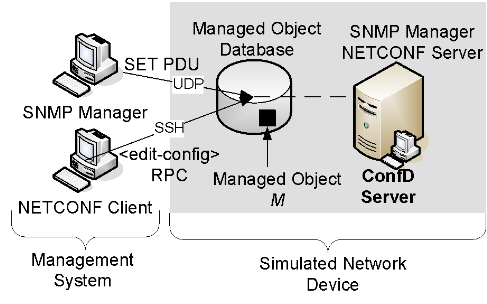
\includegraphics{Figures/netconfvssnmp1.png}}%
	\caption[Topología utilizada en las pruebas de.]{Topología utilizada en las pruebas de \parencite{netconfvssnmp}.}
	\label{fig:netconfvssnmp1}
\end{figure}

Las pruebas realizadas por los autores arrojan los resultados observados en la figura \ref{fig:netconfvssnmp2}, donde M representa la cantidad de operaciones a realizar por parte del servidor. Los autores mencionan que en los resultados obtenidos no se tiene en cuenta la carga que tienen los paquetes debido a la seguridad que ofrece el transporte \textit{SSH} por parte de \textit{NETCONF}, tampoco la carga que presenta \textit{TCP} (\textit{NETCONF}) frente a \textit{UDP} (\textit{SNMP}), entre otros.

\begin{figure}[th]
	\centering 
	\resizebox{1\textwidth}{!}{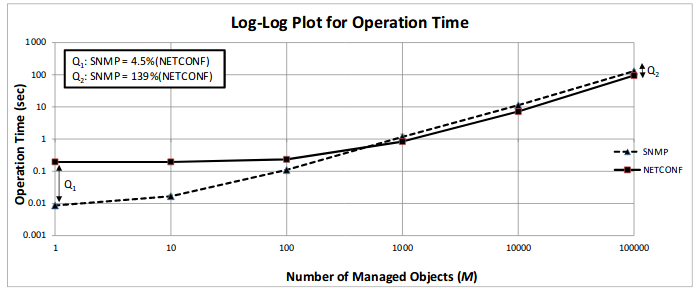
\includegraphics{Figures/netconfvssnmp2.png}}%
	\caption[Resultados obtenidos en.]{Resultados obtenidos en \parencite{netconfvssnmp}.}
	\label{fig:netconfvssnmp2}
\end{figure}

En las conclusiones de este artículo mencionan que \textit{NETCONF} es una clara alternativa a \textit{SNMP} en ámbitos de gestión de la configuración de la red. Además, destacan las bondades que presenta el protocolo \textit{NETCONF} frente a \textit{SNMP} para los proveedores de servicio como ser la seguridad de los mensajes mediante \textit{SSH}, la capacidad de revertir una configuración, el transporte de los mensajes mediante un protocolo orientado a la conexión, etc.



% tesis granada
\subsubsection*{\textit{Evaluating the Network Management Capabilities of YANG and NETCONF}}

En el artículo \parencite{netconfvstodos} se realiza un estudio de las diferentes alternativas existentes en el ámbito de la configuración y gestión de la red. A su vez, el autor desarrolla un prototipo de servidor \textit{NETCONF}. Los experimentos realizados por el autor tienen como objetivo determinar la capacidad que tienen los diferentes protocolos de gestión de configuración y monitoreo para adaptarse a entornos de \textit{SDN} y \textit{NFV}. 

Así, separa las pruebas realizadas en dos partes. En primer lugar, evalúa alternativas que permiten la configuración de un dispositivo de red. Luego, realiza un análisis de las alternativas relacionadas al monitoreo de un equipo de red.

La figura \ref{fig:netconfvstodos1} muestra una gráfica de los resultados obtenidos para el primer caso, donde concluye que \textit{NETCONF} se adapta bien a los entornos \textit{NFV} ya que se encuentra específicamente diseñado para la configuración de los equipos. Sin embargo, menciona que puede presentar dificultades adaptar el protocolo \textit{NETCONF} a entornos \textit{SDN} ya que no cumple estrictamente con el paradigma de las \textit{SDN}, donde el plano de control y el plano de datos se encuentran desacoplados íntegramente.

Por otra parte, la figura \ref{fig:netconfvstodos2} muestra el análisis para el segundo caso, en donde se evalúan protocolos y alternativas para el monitoreo de la red. En este caso, el autor menciona que si bien \textit{NETCONF} permite monitoreo en entornos \textit{NFV} y \textit{SDN}, el uso enfocado explícitamente a esta tarea no presenta mejores resultados que, por ejemplo, \textit{SNMP}.


\begin{figure}[H]
	\centering 
	\resizebox{0.8\textwidth}{!}{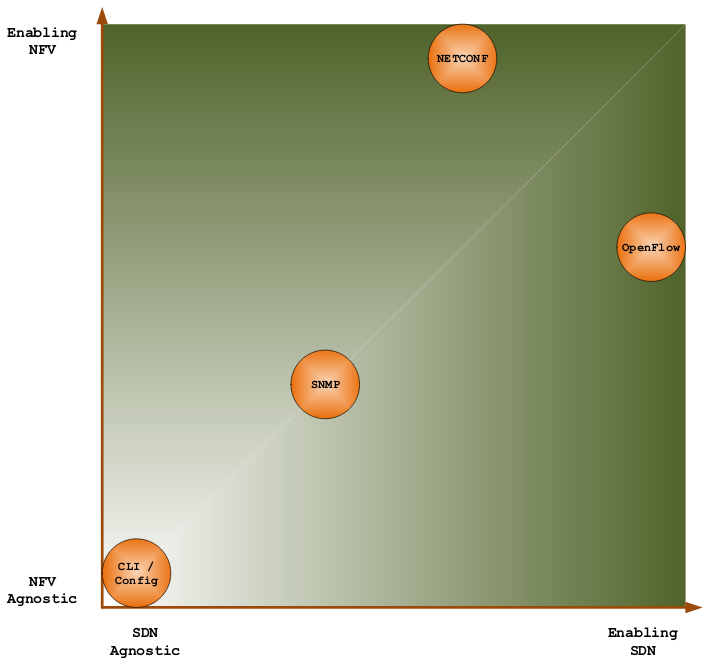
\includegraphics{Figures/netconfvstodos1.png}}%
	\caption[\textit{NETCONF} como protocolo para la administración.]{\textit{NETCONF} como protocolo para la administración \parencite{netconfvstodos}.}
	\label{fig:netconfvstodos1}
\end{figure}

\begin{figure}[H]
	\centering 
	\resizebox{0.8\textwidth}{!}{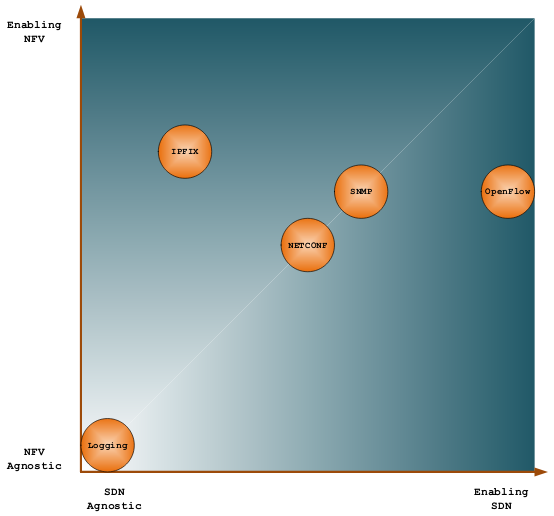
\includegraphics{Figures/netconfvstodos2.png}}%
	\caption[\textit{NETCONF} como protocolo para el monitoreo.]{\textit{NETCONF} como protocolo para el monitoreo \parencite{netconfvstodos}.}
	\label{fig:netconfvstodos2}
\end{figure}



% tesis granada% tesis granada% tesis granada% tesis granada% tesis granada
\subsubsection*{\textit{Control and Management of Transponders With NETCONF and YANG}}

El documento \parencite{netconfsddn} propone la utilización del protocolo de administración \textit{NETCONF} en un ambiente \textit{SDN} para administrar la configuración de un \textit{transponder}, sugiriendo un entorno como el que se puede ver en la figura \ref{fig:netconfsddn1}.


\begin{figure}[H]
	\centering 
	\resizebox{1\textwidth}{!}{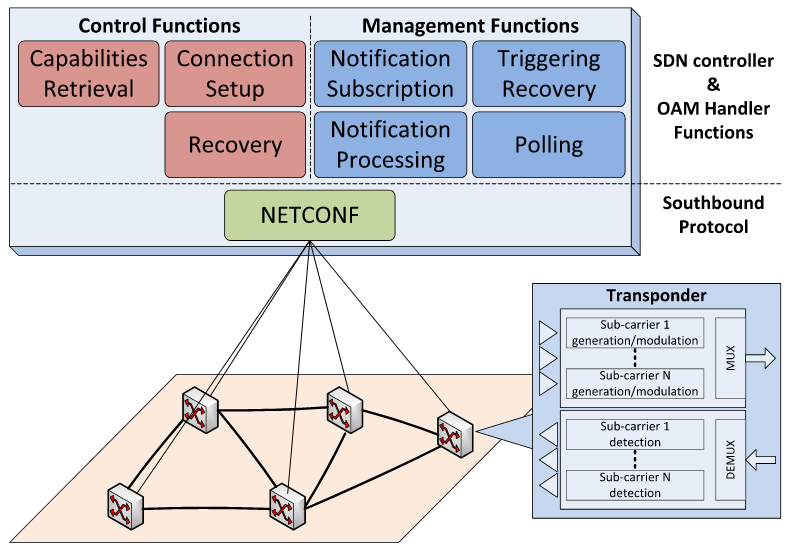
\includegraphics{Figures/netconfsddn1.png}}%
	\caption[Topología propuesta en.]{Topología propuesta en \parencite{netconfsddn}.}
	\label{fig:netconfsddn1}
\end{figure}

Sin embargo, finalmente realizan una demostración compuesta por dos \textit{transponders} y un \textit{switch}, los tres virtuales y sin utilización de algún controlador \textit{SDN}. Esta última topología se muestra en la figura \ref{fig:netconfsddn2}.


\begin{figure}[H]
	\centering 
	\resizebox{0.55\textwidth}{!}{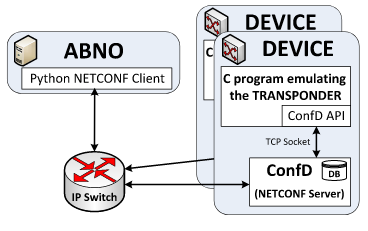
\includegraphics{Figures/netconfsddn2.png}}%
	\caption[Escenario propuesto para las pruebas en.]{Escenario propuesto para las pruebas en \parencite{netconfsddn}.}
	\label{fig:netconfsddn2}
\end{figure}

Los autores concluyen que \textit{NETCONF} como protocolo de gestión y \textit{YANG} como modelado de datos, son estándares viables para la configuración, gestión y monitoreo de los datos en dispositivos de red como los \textit{transponders}. 
Además, resaltan el alto rendimiento obtenido en sus pruebas para la configuración y monitoreo de los \textit{transponders} haciendo uso de estos protocolos. 


\section{Objetivos propuestos}

El objetivo general de este proyecto integrador es adquirir los conocimientos relacionados con administración de redes, particularmente con el esquema conocido como Redes Definidas por Software y el protocolo de administración de la configuración \textit{NETCONF}. Para esto, se propone usar como vehículo de prueba un entorno constituido por ambas tecnologías para lograr la administración y monitoreo del estado de un \textit{muxponder}. Se prestará particular atención al estudio y comparación de las diferentes opciones abiertas disponibles para la implementación del protocolo \textit{NETCONF}.

\subsection{Objetivos particulares}

Las tareas a realizar en este trabajo de fin de grado llevarán a:


\begin{itemize}
    \item Adquirir un amplio conocimiento de las tecnologías existentes en \textit{SDN}.   
    \item Tener un conocimiento acabado en el protocolo de administración de red \textit{NETCONF}.   
    \item Desarrollar una librería en el controlador \textit{SDN} que permita la comunicación, a través de \textit{NETCONF}, con un dispositivo óptico.   
    \item Compilar e instalar en un dispositivo óptico un agente del protocolo \textit{NETCONF} y una librería que relacione las variables de configuración y estado del dispositivo con dicho agente.   
    \item Desarrollar una aplicación de interfaz de usuario para administrar de manera simple los dispositivos de red.
\end{itemize}  
    
\section{Estructura del texto}

Aquí se listan los distintos capítulos que conforman el proyecto, presentando una breve descripción de su contenido. El escrito está compuesto por 6 capítulos, los apéndices y la bibliografía.


\begin{itemize}   
    \item \textbf{Capítulo 1 - Introducción:} Se exponen en este capítulo los aspectos más significativos del proyecto, donde se incluye las motivaciones que llevaron a realizar el mismo junto con una revisión del estado del arte relacionado y los objetivos propuestos para el trabajo de fin de grado.

    \item \textbf{Capítulo 2 - Marco teórico:} Aquí se abordan los conceptos necesarios para comprender las tecnologías utilizadas por el proyecto, además los mismos presentan una fundamentación para las posteriores implementaciones prácticas.

    \item \textbf{Capítulo 3 - Análisis de las tecnologías:} Se estudia y analiza en este capítulo todas las herramientas que permiten la implementación de las aplicaciones desarrolladas en este proyecto, abarcando tanto herramientas de software como de hardware.

    \item \textbf{Capítulo 4 - Diseño e implementación:} En este capítulo se abordan los procesos de diseño e implementación de todas las aplicaciones realizadas. Se presentan los requerimientos de las mismas y los diferentes diagramas realizados que explican el funcionamiento de cada pieza de software. 

    \item \textbf{Capítulo 5 - Validación y verificación:} Aquí, se exponen los diferentes casos de prueba desarrollados con el objetivo de validar y verificar que se cumplan los requerimientos de las diferentes aplicaciones.

    \item \textbf{Capítulo 6 - Conclusión:} Se presenta en este capítulo las conclusiones obtenidas tras la realización del trabajo, posibles vías de trabajos futuros y una apreciación personal del proceso abordado.
	
	\item \textbf{Apéndices:} En los apéndices se proporciona al lector un tutorial de como desplegar el entorno de trabajo y las aplicaciones desarrolladas en este proyecto.
    
    \item \textbf{Bibliografía:} En esta parte final del documento, se muestran todas las referencias que se han consultado para el desarrollo del proyecto.   
\end{itemize}


 % Chapter Template
% cSpell:words parencite 
\chapter{Marco teórico} % Main chapter title 

\label{Chapter2} % Change X to a consecutive number; for referencing this chapter elsewhere, use \ref{ChapterX}
En este capítulo se comprenderán conceptos teóricos sobre las tecnologías claves en las cuales se basa el proyecto. Como introducción, se analizará el funcionamiento de las redes tradicionales, donde se dejará en evidencia la necesidad de un nuevo paradigma. 

Luego, se analizarán los fundamentos en los que se basan las Redes Definidas por Software y por qué este paradigma resuelve los problemas presentados por el enfoque de las redes tradicionales. 

También, se introducirán conceptos de lenguajes de modelado y se abordará la importancia de la gestión de la red. Se estudiará \textit{NETCONF} como protocolo de gestión de red. Finalmente, se abordan conceptos de dispositivos ópticos de transporte.

%----------------------------------------------------------------------------------------
%	SECTION 1
%----------------------------------------------------------------------------------------
\section{Redes tradicionales} \label{sec:rdtr}

La infraestructura actual de las redes tradicionales basan su funcionamiento íntegramente en los dispositivos de red \parencite{ISACA}. Cada dispositivo lleva su propia gestión sobre el plano de datos y el plano de control de manera local y comunica a los demás dicha información de ser necesario. 

Un ejemplo de esto se puede observar en la figura \ref{fig:dev_tradicional}, donde dos dispositivos intercambian información referente al plano de control.


\begin{figure}[H]
	\centering
	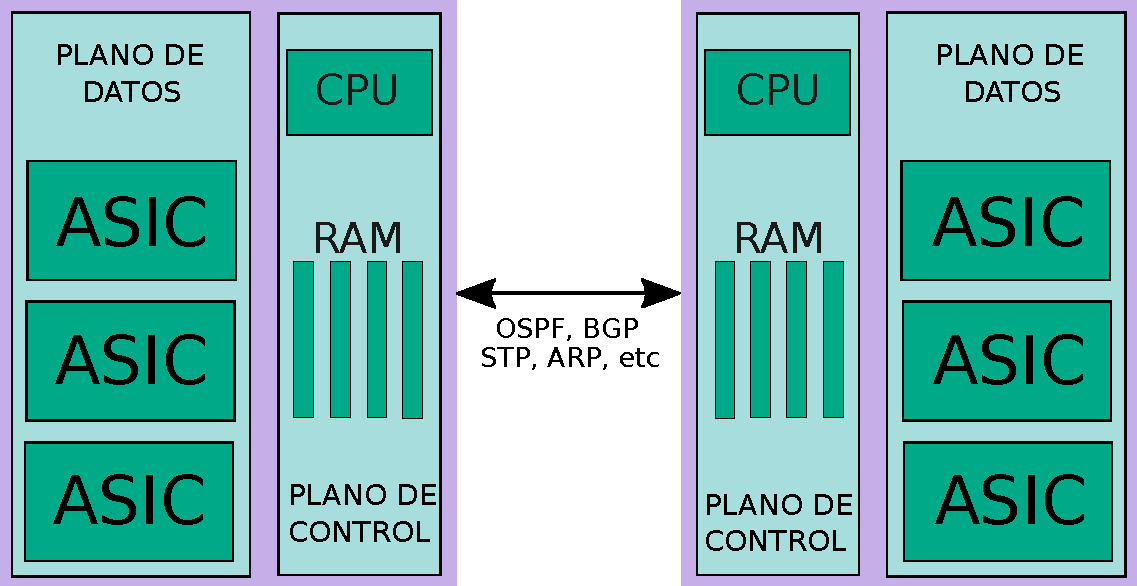
\includegraphics[scale=0.60]{Figures/dispositivo-tradicional.pdf}
	\caption{Comportamiento de dispositivos en redes tradicionales.}
	\label{fig:dev_tradicional}
  \end{figure}


\subsection{Plano de Control}
Comprende la configuración del sistema, la administración y el intercambio de información de ruteo entre los dispositivos \parencite{ControlPlane}. Es el responsable de administrar la configuración del equipo y de programar el camino que será usado para el flujo de los paquetes. En otras palabras, es en este plano donde se calculan y se toman las decisiones de enrutamiento y reenvío. En las redes tradicionales, cualquier aplicación que utilice el dispositivo para administrar su configuración reside en esta capa. 

El proceso de establecimiento de la topología de red utilizando un plano de control que se ejecuta localmente, es compleja debido a que no existe ningún dispositivo que sea conocido por toda la red. Para gestionar cambios o actualizaciones en cada dispositivo se debe estar conectado a su plano de control de forma individual, lo que no resulta en un enfoque inteligente.

\subsection{Plano de Datos}
También conocido como plano de usuario o plano de reenvío \parencite{DataPlane}, es el encargado de transportar el tráfico de usuario hacia el destinatario final. Una diferencia importante que tiene el tráfico correspondiente al plano de datos con respecto al plano de control, es que el primero es generado en los terminales mientras que en el segundo caso, el tráfico es generado en los dispositivos de red. Tiene como objetivo el reenvío de los paquetes hacia el próximo salto basándose en las decisiones tomadas por la capa de control.
\\


El enfoque dado por las redes tradicionales cumplió con las necesidades de una época donde las arquitecturas cliente-servidor eran dominantes. Tiene como ventaja ser simple a nivel lógico, mientras que el plano de control implica el uso de microprocesadores para tratar los paquetes y conformar las tablas, el plano de datos se desarrolla en silicio. A pesar de ello, presenta una serie de problemas \parencite{onfwhitepaper}:

\begin{itemize}
	\item \textbf{Funcionalidad de la red integrada en los dispositivos:} El plano de control se encuentra íntegramente en los dispositivos de red, lo que resulta en una configuración de red estática, inflexible y descentralizada. 
	\item \textbf{Escalabilidad:} La escalabilidad resulta afectada y no apropiada para la explosión de las nuevas tecnologías como \textit{Big Data}, \textit{Cloud Computing} y el \textit{Streaming}, donde la complejidad de la red incrementa rápidamente debido a que cada dispositivo agregado debe ser configurado y administrado.
	\item \textbf{Políticas inconsistentes:} Si las políticas de configuración cambian a nivel de red, implica un cambio en todos los dispositivos que la componen por parte de los administradores de red.
	\item \textbf{Dependencia del fabricante y personalización:} El plano de control integrado a los dispositivos de red resulta en una dependencia a los ciclos de producción de equipamientos por parte de los fabricantes para incorporar nuevas funcionalidades. Además, con la finalidad de asegurar la calidad de servicio y brindar alta perfomance, la industria define los protocolos de red de forma específica y aislada, sin el beneficio de una acción conjunta e incapacitando a los operadores a personalizar la red para sus entornos individuales y específicos. 
\end{itemize}

%----------------------------------------------------------------------------------------
%	SECTION 2
%----------------------------------------------------------------------------------------
\section{Redes Definidas por Software} \label{sec:rsdn}

A diferencia de las aplicaciones y los nuevos requerimientos de los usuarios, las redes no han cambiado mucho respecto a los últimos 30 años \parencite{sdnroad}. El desarrollo de las \textit{SDN} se inició en 1990 donde se introdujo el concepto de funciones programables en la red, teniendo gran innovación en 2001-2007 donde se propone separar el plano de datos del plano de control. El próximo gran paso de las \textit{SDN} llegó en 2007-2010, con la implementación de la \textit{API OpenFlow}.
\\

Las redes definidas por software nacen en respuesta a la dinámica y flexibilidad que requieren las nuevas tendencias, donde el enfoque presentado por las redes tradicionales no cumple dado su naturaleza estática. 

\subsection{Definición de \textit{SDN}}
Según la \textit{ONF} \parencite{onfwhitepaper}, la red definida por software, también conocida como red programable o automatizada, consiste en una arquitectura donde el plano de datos se encuentra separado del plano de control y donde este último a su vez puede controlar varios dispositivos.

Tal como destaca \textit{SDx Central} en su reporte \parencite{SDXCentralReport}, este nuevo paradigma presenta las siguientes ventajas:

\begin{itemize}
	\item \textbf{Plano de control centralizado:} A diferencia del enfoque presentado por las redes tradicionales donde se tenía un plano de control distribuido entre los diferentes equipos que conforman la red, ahora se tiene un plano de control centralizado y presente a nivel lógico en un mismo punto. De esta forma, se tiene una visión general y global de toda la red, relajando las comunicaciones entre los dispositivos y las complejidades introducidas por las configuraciones individuales de cada uno. Además, el plano de control ahora es directamente programable, sin tener que usar como intermediario el plano de datos. Todo el tráfico ahora está bajo la supervisión de este nuevo plano de control centralizado, transformando a la red en una red programable. 
	\item \textbf{Costos:} Los costos relacionados al control de la gestión del tráfico y de configuración de los diferentes equipos se ven reducidos en tiempo y esfuerzo dado el plano de control centralizado.
	\item \textbf{Automatización:} Un beneficio indirecto de tener un plano de control centralizado, es poder tomar diferentes decisiones y políticas en base a la visibilidad global de la red en tiempo real, aplicando configuraciones en los diferentes equipos de forma automática.
	\item \textbf{Escalabilidad:} \textit{SDN} admite topologías dinámicas con capacidades para adaptarse a cambios, debido a la automatización de la configuración de los dispositivos. Con la capacidad de ajustar los picos y las bajas en la carga del tráfico, las empresas pueden crear e implementar nuevos servicios y aplicaciones sin demora debido a la infraestructura más flexible.
	\item \textbf{Mantenimiento y monitoreo:} Por medio del controlador \textit{SDN} se puede conocer, en cualquier momento, el estado actual de la red incluyendo los dispositivos que la componen.
	\item \textbf{Seguridad:} Dado que la administración de toda la red se realiza en un solo punto, se asegura que no existan debilidades o inconsistencias en las configuraciones de las aplicaciones y los equipos.
\end{itemize}

\subsection{Arquitectura de \textit{SDN}}
En las redes tradicionales, cada dispositivo tiene integrado tanto el plano de datos como el plano de control. En \textit{SDN}, el plano de datos se encuentra desacoplado del plano de control y, además, se puede diferenciar un nuevo plano llamado \textit{plano de aplicación} \parencite{onfsdnarq}. A continuación, se analizará cuál es la función que cumple cada plano en esta nueva arquitectura propuesta por las \textit{SDN}.

\subsubsection{Plano de Datos}
Comprende la misma funcionalidad que en las redes tradicionales. Consiste en un conjunto de dispositivos de red con funcionalidades de reenvío de paquetes.

\subsubsection{Plano de Aplicación}
Con el enfoque de las redes tradicionales, el plano de aplicación se encontraba integrado en el plano de control. En \textit{SDN}, el plano de aplicación se desacopla al igual que el plano de control. En este plano se encuentran las aplicaciones de red que implementan las funcionalidades de más alto nivel y que participan en las decisiones de administración y control de ruteo.

\subsubsection{Plano de Control}
Toda la función de control se encuentra centralizada fuera de los dispositivos, permitiendo a los desarrolladores de aplicaciones utilizar las capacidades de la red pero haciendo una abstracción de su topología o sus funciones. Tiene como objetivo mediar, organizar y facilitar la comunicación entre los diferentes equipos y las aplicaciones. Además, este plano ahora está disponible para poder ser programado desde un software externo al controlador.
\\

En la figura \ref{fig:arquitectura_sdn}, se expone la anatomía de un controlador \textit{SDN}. En ella, se puede observar dos interfaces comprendidas por el plano de control \parencite{sdnarqsouth}: \textit{Southbound} y, \textit{Northbound}.

\begin{itemize}
	\item \textbf{\textit{Southbound API}:} necesaria por la separación del plano de control del plano de datos. Define la \textit{API} de comunicación entre el controlador y los diferentes dispositivos de red, en otras palabras, entre el plano de control y el plano de datos.  
	\item \textbf{\textit{Northbound API}:} funciona como interfaz tanto de alto como de bajo nivel, es necesaria para permitir que las aplicaciones que se ejecutan en la parte superior de \textit{SDN} puedan comunicarse con el mismo. En el primer caso, la interfaz provee una abstracción de la red en sí misma, permitiendo a los desarrolladores no tener que preocuparse por los dispositivos individuales, sino manejar la red como un todo. En el segundo caso, la interfaz advierte a las aplicaciones sobre la existencia de los dispositivos individuales y sus enlaces, pero oculta las diferencias entre los dispositivos. 
\end{itemize}


\begin{figure}[htbp]
	\centering
	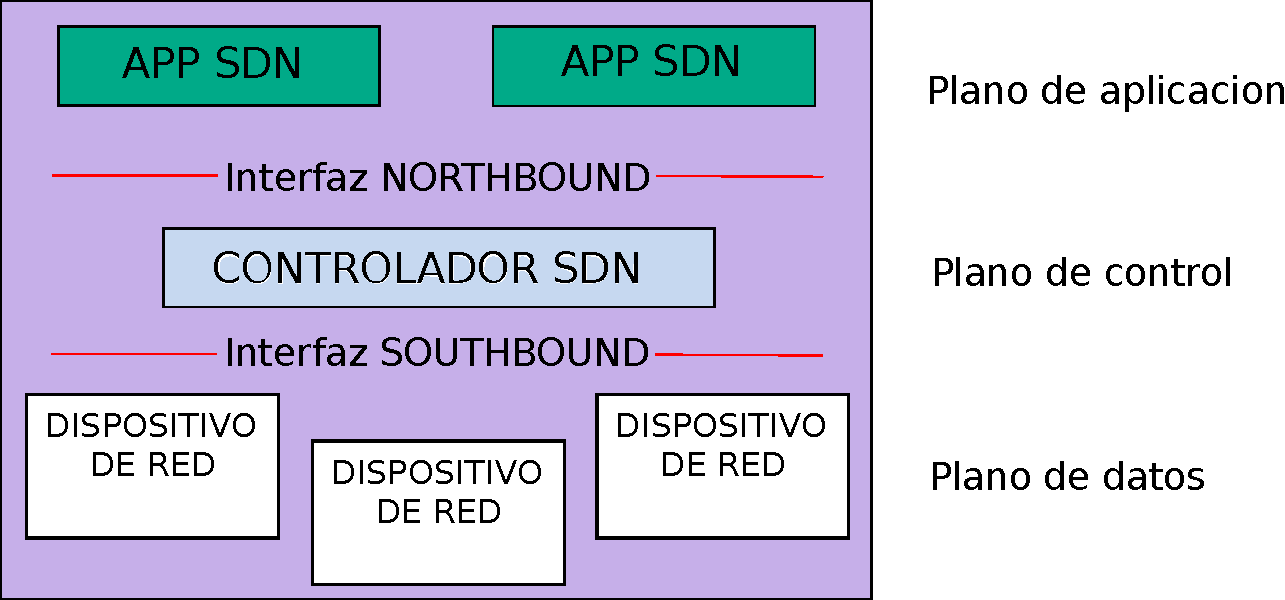
\includegraphics[scale=0.6]{Figures/arquitectura-controlador.pdf}
	\caption{Arquitectura de un controlador \textit{SDN} tradicional.}
	\label{fig:arquitectura_sdn}
  \end{figure}

%----------------------------------------------------------------------------------------
%	SECTION 3
%----------------------------------------------------------------------------------------
\section{Gestión de la Red} \label{sec:gestionred}
En la actualidad se puede encontrar una gran variedad de redes, desde pequeñas redes domésticas de intranet hasta redes empresariales o de proveedores de servicios. Cada una de estas redes tienen diversos requerimientos de gestión.  Las pequeñas redes domésticas, que consisten en unos pocos dispositivos conectados, requieren una sobrecarga de administración baja, y con frecuencia, pueden gestionarse manualmente de forma eficiente. No así las redes más grandes, que podrían contener cientos dispositivos conectados requiriendo un enfoque más sistemático para hacer frente a las complejidades que surgen debido al tamaño de la red. A medida que la red crece en estructura y complejidad, se hace evidente la necesidad de una solución eficiente para la gestión de la misma \parencite{gestionderedes}.

\subsection{Protocolos de Gestión}
Existen múltiples formas de llevar a cabo la administración de la configuración en los diversos dispositivos que conforman la red. En esta sección, se analizarán dos alternativas: \textit{CLI} y \textit{SNMP}.

\subsubsection{\textit{Command Line Interface}}
\textit{CLI} es el enfoque más común en el ámbito de gestión de la configuración, adoptado por múltiples empresas. Está orientado a que resulte fácil de entender para las personas, presentando una interfaz de texto simple. Sin embargo, no se encuentra orientado a las \textit{API’s}, donde la implementación interna podría ser diferente entre los distintos dispositivos, incluso entre dispositivos del mismo fabricante. La \textit{CLI} puede utilizar \textit{API’s} internas para cambiar la lógica de la función de red o bien podría transformar los comandos ingresados en un archivo de configuración y reiniciar la configuración del dispositivo con dicho archivo.
\\

Un ejemplo de una operación en \textit{CLI} puede verse en la figura \ref{fig:cli}
\\
\begin{figure}[htbp]
	\centering
	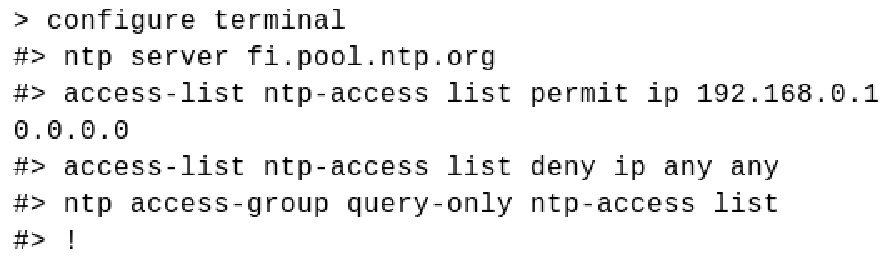
\includegraphics[scale=0.7]{Figures/cli.pdf}
	\caption{Interacción tipica con un dispositivo mediante \textit{CLI}.}
	\label{fig:cli}
  \end{figure}

  Este enfoque presenta una serie desventajas \parencite{clilimitacion}. En primer lugar, la implementación de las \textit{API’s} \textit{CLI} no están estandarizadas, por lo que las operaciones varían drásticamente entre dispositivos de diferentes fabricantes e incluso en implementaciones \textit{CLI} del mismo fabricante. A su vez, los fabricantes podrían brindar una actualización de software del dispositivo donde los comandos \textit{CLI} de la versión anterior se vean modificados o eliminados, lo que no solo se traduce a problemas para el administrador de red, sino también para las \textit{API} que usen la \textit{CLI}. En segundo lugar, algunas operaciones en la gestión de la configuración podrían requerir múltiples transacciones \textit{CLI}, si alguna de estas transacciones falla, el dispositivo podría quedar en un estado inconsistente. \textit{CLI} no define de forma estándar una solución para deshacer los cambios aplicados en el dispositivo.

  \subsubsection{\textit{Simple Network Management Protocol}}
  \textit{SNMP} es un protocolo de monitoreo y administración de red, estandarizado por primera vez en 1988 por la \textit{IETF} \parencite{snmprfc}. Su funcionamiento se basa en una arquitectura cliente-servidor, donde los mensajes se intercambian a través del protocolo de transporte no orientado a la conexión \textit{UDP}. Consiste en una colección de agentes y administradores formando entre ellos una red, donde se denomina administrador a aquel dispositivo que tiene el rol de ejecutar aplicaciones de administración de red, mientras que los dispositivos que requieran ser administrados se denominan agentes \parencite{snmprfcfunc}.

  Las capacidades para administrar la red en \textit{SNMP} quedan representadas en lo que se conoce como \textit{MIB}. Una \textit{MIB} es una base de datos que contiene información jerárquica y estructurada en forma de árbol de todos los parámetros gestionables de la red. 
  Dicha base de datos se debe cargar en el administrador \textit{SNMP}, para ello cada agente \textit{SNMP} expone al administrador \textit{SNMP} una serie de módulos \textit{MIB}. Con esta información el administrador podría alterar dinámicamente la configuración del agente. 
  \\

  El uso de \textit{SNMP} como monitoreo es una práctica común desde su publicación, sin embargo, se desalentó su uso en áreas de gestión de configuración por las siguientes razones \parencite{snmplimitacion}: 

  \begin{itemize}
	\item Problemas inherentes al protocolo de transporte \textit{UDP}, donde los mensajes pueden perderse o llegar desordenados, así como también la falta de mecanismos de seguridad para los mismos jugaron un papel importante para reemplazar \textit{SNMP} por otros protocolos de administración de red.
	\item No existe una estandarización de los módulos \textit{MIB} para configurar las funciones de red. El trabajo de descubrir correctamente los módulos \textit{MIB} para cada dispositivo es tarea del usuario, lo que resulta compleja y no eficiente.
\end{itemize}

\subsubsection{Otras alternativas}
Algunos enfoques para la gestión de la red pueden incluir soluciones basadas en páginas web, que permiten al administrador modificar las configuraciones en el dispositivo de forma gráfica y más amigable, pero generalmente resultan más limitadas que las \textit{CLI}. 
Además, algunos dispositivos pueden brindar soluciones propietarias para la gestión de la configuración, sin embargo, estas soluciones suelen ser muy específicas a un dispositivo o una familia de dispositivos, y rara vez suelen ser compatibles entre sí. Estos últimos también representan una carga para los administradores, donde cada solución requiere que el administrador aprenda otra manera de configurar las funcionalidades de la red.  

\subsection{\textit{NETCONF}}
Esta sección repasa brevemente los conceptos y características principales que ofrece el protocolo \textit{NETCONF}. Además, aspectos de seguridad, transporte y control de acceso del protocolo se discuten en detalle. 

\subsubsection{Definición}
\textit{NETCONF} fue estandarizado por la \textit{IETF} por primera vez en el 2006, en el \textit{RFC 4741} \parencite{netconfrfc}. Actualmente está siendo adoptado por los principales proveedores de dispositivos de red y ha ganado el apoyo de la industria. Según detalla Carl Moberg \parencite{netconfusos}, podemos encontrar que fabricantes como Juniper, Huawei, Cisco, entre otros, brindan soporte desde hace tiempo del protocolo \textit{NETCONF}. 
\\

La \textit{IETF} definde a \textit{NETCONF} como un protocolo estándar para Instalar, manipular y borrar configuraciones en un dispositivo \parencite{netconfrfcnuevo}. Permite implementar una \textit{API} formal utilizando el lenguaje de modelado \textit{YANG} para administrar y monitorear las funcionalidades de la red. \textit{NETCONF} utiliza el paradigma de las \textit{RPC}, donde construye los mensajes que intercambian información como un flujo con codificación \textit{XML}. Funciona con una arquitectura cliente-servidor, donde los mensajes son transportados utilizando algún protocolo orientado a la conexión. El \textit{RFC 6241}, en la sección 1.2, menciona una partición conceptual del protocolo en cuatro capas, dicha partición se refleja en la figura \ref{fig:netconf}. 

A continuación, se explica qué función cumple cada una de estas capas.

\begin{itemize}
	\item \textbf{Capa de transporte seguro:} provee mecanismos de comunicación entre cliente y servidor.  
	\item \textbf{Capa de mensajes:} encargada de la codificación y partición de los mensajes.  
	\item \textbf{Capa de operación:} define las operaciones admitidas por el protocolo.
	\item \textbf{Capa de contenido:} relaciona la representación y el modelado de los datos en el protocolo.    
\end{itemize}

\begin{figure}[htbp]
	\centering
	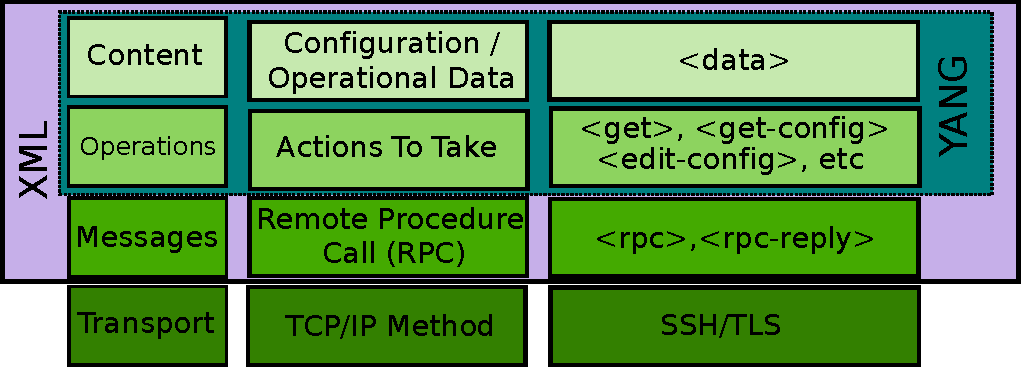
\includegraphics[scale=0.9]{Figures/stack-netconf.pdf}
	\caption{Separación conceptual del protocolo \textit{NETCONF}.}
	\label{fig:netconf}
  \end{figure}


  Las características que destacan a \textit{NETCONF} como protocolo de administración de red son \parencite{netconfpros}:

  \begin{itemize}
	\item Capacidad de restauración de los datos y \textit{backup} de la configuración.
	\item De uso fácil, presentando la información de forma estructurada con una codificación entendible para las personas y las \textit{API’s}.
	\item Implementa mecanismos de control de errores mediante validación de sintaxis y semántica.
	\item Separación clara de los datos de configuración y los datos de estado.
	\item Posibilidad de gestionar la configuración en un dispositivo de manera reactiva mediante notificaciones del mismo.
\end{itemize}

\textit{NETCONF} separa los datos de configuración de los datos de estado de un dispositivo. Según lo detallado en la sección 1.1. y 1.4 del \textit{RFC 6242}, se define a cada uno como:

\begin{itemize}
	\item \textbf{Datos de configuración:} información que se puede leer o escribir y que se utiliza para llevar al dispositivo de un estado inicial a un estado deseado. Un ejemplo es la velocidad del ventilador del cpu del dispositivo.  
	\item \textbf{Datos de estado:} representa información de sólo lectura y estadísticas brindadas por el dispositivo. Por ejemplo, la temperatura del cpu del equipo.   
\end{itemize}

\subsubsection{Conceptos del Protocolo}
Como se mencionó anteriormente, \textit{NETCONF} define un protocolo de administración de red con arquitectura cliente-servidor, donde el cliente en este caso es el sistema de administración de la red o el administrador del sistema, mientras que el dispositivo que contiene una o más funciones de red que deben ser administradas, actúa de servidor. El cliente y el servidor inician la sesión de protocolos mediante un primer mensaje que da lugar al intercambio de capacidades o \textit{capabilities}, donde se definen qué operaciones estarán disponibles para su uso. Este primer mensaje recibe el nombre de \textit{HELLO} \parencite{netconfrfcnuevo}. La figura \ref{fig:netconf_comunicacion} ejemplifica la arquitectura presentada por el protocolo.

\begin{figure}[htbp]
	\centering
	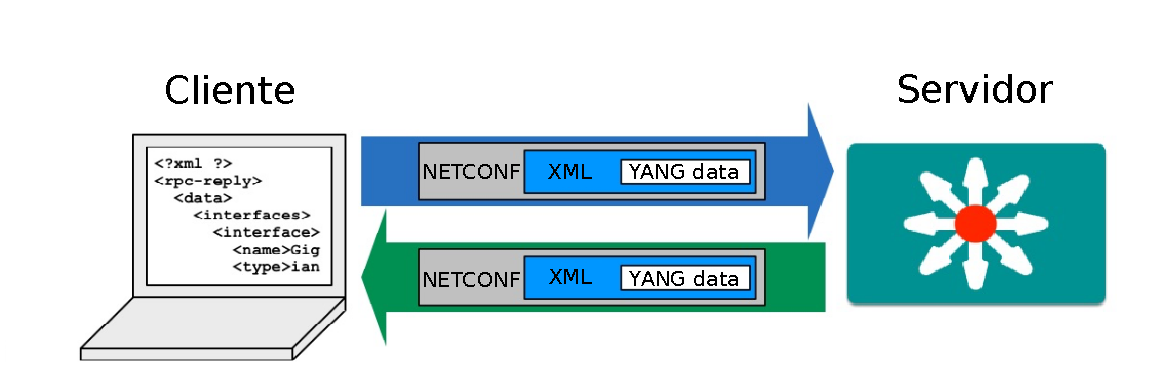
\includegraphics[scale=0.8]{Figures/netconf-cliente-servidor.pdf}
	\caption{Arquitectura cliente-servidor en el protocolo \textit{NETCONF}.}
	\label{fig:netconf_comunicacion}
  \end{figure}

  \subsubsection{Capacidades}
  El protocolo \textit{NETCONF} está diseñado para ser altamente extensible y, con este fin, es compatible con el intercambio inicial de capacidades entre cliente y servidor \parencite{netconfrfcnuevo}. Este intercambio de información permite al cliente ajustar sus comportamientos basándose en las funcionalidades que admite el servidor. Cada capacidad establecida por el protocolo recibe un nombre asignado por la \textit{IANA}. Además, también se incluye el intercambio de los modelos \textit{YANG} que tiene implementado el servidor, lo cual es necesario no solo para que el cliente pueda aprender de los mismos, sino también para reconocer las diferentes revisiones implementadas en el servidor.

  \subsubsection{Sesión orientada a la conexión}
  La sección dos del \textit{RFC 6242}, referida a protocolos de transporte, detalla que \textit{NETCONF} no esta vinculado a ningún protocolo de transporte específico. El requisito necesario de \textit{NETCONF} para el protocolo de transporte subyacente es que el mismo sea orientado a la conexión. 

  \subsubsection{Sesión orientada a la autenticación}
  El protocolo \textit{NETCONF} es orientado a la sesión con autenticación, utilizando una arquitectura cliente-servidor donde el servidor escucha un puerto asignado para recibir las conexiones con los clientes. 

  Según la sección dos del \textit{RFC 6242} referida a seguridad, el protocolo mínimamente debe ofrecer autenticación, confidencialidad e integridad. Cualquier mensaje \textit{NETCONF}, incluido el mensaje \textit{HELLO}, se envian unicamente si el cliente y servidor se han autenticado de forma correcta. No se especifica un protocolo en particular, pudiendo utilizarse alguno de los múltiples protocolos de transporte seguros existentes en la actualidad como \textit{TLS}, \textit{SSH}, \textit{BEEP}, etc. Cualquier implementación de \textit{NETCONF} debe, al menos, soportar \textit{SSH} como protocolo de transporte seguro.

  Además, según el \textit{RFC 6536} relacionado al control de acceso de usuarios, \textit{NETCONF} admite una jerarquía de niveles de usuarios. Por ejemplo, tener dos grupos de usuarios donde uno tenga permisos de configuración más limitados que el otro.

  \subsubsection{Bases de datos}
  \textit{NETCONF} define en la sección cinco del \textit{RFC 6242}, la existencia de uno o más \textit{datastores}, los cuales cumplen el papel de una base de datos conceptual que puede ser utilizada para almacenar y acceder tanto a los datos de configuración como a los datos de estado. El protocolo especifica y define tres tipos de base de datos: \textit{running}, \textit{startup} y \textit{candidate}, de las cuales únicamente es obligatorio que se implemente la primera. Si la implementación admite otras bases de datos, como por ejemplo \textit{startup} o \textit{candidate}, el servidor informará al cliente esta capacidad en el mensaje \textit{HELLO}. Cada operación en \textit{NETCONF} debe especificar la base de datos a la cual se realizará la consulta o modificación.
  \\

  A continuación, se detalla cada uno de los almacenes de datos mencionadas.
\begin{itemize}
	\item \textbf{\textit{startup}:} según lo especificado en la sección 8.7 del \textit{RFC 6242}, dicha base de datos se utiliza para almacenar de forma persistente la información de configuración del dispositivo. El contenido de esta es copiado de manera automática a la base de datos conocida como \textit{running} en el inicio del servidor \textit{NETCONF}. 
	\item \textbf{\textit{running}:} refleja la configuración actualmente en uso por el dispositivo. Es la única base de datos conceptual que admite la presencia tanto de datos de estado como datos de configuración. 
	\item \textbf{\textit{candidate}:} se encuentra definido en la sección 8.3 del \textit{RFC 6242}. Puede ser utilizado para realizar cambios que no se van a aplicar al dispositivo de forma directa, sino que lo harán una vez se realice un \textit{commit} sobre dicha base de datos. De esta forma, el contenido de \textit{candidate} es copiado a \textit{running}. Si de lo contrario se desea descartar los cambios realizados en este \textit{datastore}, la operación \textit{discard-changes} copia el contenido de \textit{running} a \textit{candidate}. En esta base de datos conceptual únicamente se admiten datos de configuración.
\end{itemize}


Como se mencionó anteriormente, cualquier implementación de \textit{NETCONF} debe admitir al menos el \textit{datastore running}, esto es necesario ya que los datos de estado (necesarios para monitorear el dispositivo) únicamente se encuentran admitidos en dicho \textit{datastore}.

\subsubsection{Operaciones del protocolo}

Las operaciones en el protocolo \textit{NETCONF} se definen como \textit{RPC} en los modelos \textit{YANG} relevantes. En dichos modelos también se definen los argumentos de entrada y los contenidos de salida para cada operación. Todas las operaciones están codificadas en \textit{XML} dentro de los mensajes \textit{RPC} que son, de hecho, los únicos mensajes que los clientes pueden enviar en las sesiones de \textit{NETCONF} después del intercambio inicial del mensaje \textit{HELLO}. 
\\

Como las operaciones son \textit{RPC}, cada mensaje enviado por los clientes tiene una respuesta por parte del servidor. Este resultado normalmente contiene \textit{ok} para indicar que la operación resultó según lo esperado, o \textit{error} indicando las razones por la cual falló dicha operación.
\\

El protocolo define en la sección 7 del \textit{RFC 6241} nueve operaciones básicas y necesarias para cualquier implementación del mismo, las cuales se describen a continuación:

\begin{itemize}
	\item \textbf{\textit{get}:} utilizado para consultar tanto datos de configuración como datos de estado al servidor \textit{NETCONF}.
	\item \textbf{\textit{get-config}:} operación que devuelve los datos de configuración del dispositivo. Puede incluir filtros para limitar la información enviada por parte del servidor.
	\item \textbf{\textit{edit-config}:} definida para crear, actualizar o borrar datos de configuración en el servidor. Únicamente se admite esta operación en las bases de datos \textit{running} o \textit{candidate}.
	\item \textbf{\textit{copy-config}:} crea o reemplaza completamente el contenido de una base de datos por otra. El caso de uso más común de esta operación es para copiar el contenido del \textit{datastore running} al \textit{datastore startup}. 
	\item \textbf{\textit{delete-config}:} Elimina completamente el contenido de un \textit{datastore} determinado. No se admite esta operación para la base de datos \textit{running}.
	\item \textbf{\textit{lock}:} permite al cliente bloquear la configuración completa de un \textit{datastore} específico en un dispositivo. Tales bloqueos son destinados a ser de corta duración, de esta forma un cliente puede realizar un cambio sin temor a la interacción con otros clientes de \textit{NETCONF}. Además, como el protocolo es orientado a la sesión, todos los recursos tomados por la misma tales como los datastores, deben ser liberados en el momento de la finalización o cierre de la sesión.
	\item \textbf{\textit{unlock}:} permite a la sesión liberar el recurso tomado por la operación lock.
	\item \textbf{\textit{close-session}:} utilizada para finalizar la sesión entre cliente y servidor \textit{NETCONF}. Cualquiera de las operaciones mencionadas en esta sección, quedan inhabilitadas una vez finalizada la sesión.
	\item \textbf{\textit{kill-session}:} permite al administrador de red finalizar alguna sesión inactiva que tiene recursos tomados. 
\end{itemize}

Además de estas nueve operaciones descritas por el protocolo, pueden proporcionarse operaciones adicionales basado en las capacidades anunciadas por el dispositivo, como por ejemplo operaciones \textit{RPC} definidas en los módulos \textit{YANG}.
\\

También, \textit{NETCONF} admite operaciones con capacidades más avanzadas. No es obligatorio que las diferentes implementaciones del mismo soporten las siguientes características, más bien, de hacerlo deben ser expuestas como capacidades admitidas en el mensaje \textit{HELLO}. Dichas operaciones se describen a continuación:
\begin{itemize}
	\item \textbf{\textit{commit}:} operación utilizada para copiar atómicamente el contenido del \textit{datastore candidate} al \textit{datastore running}. Además, puede incluirse la operación \textit{confirmed-commit}, esta última funciona como un \textit{backup} de la configuración previa al \textit{commit}, la cual se restablece al cabo de un \textit{timeout} si no se recibe la operación \textit{confirmed-commit}. \textit{NETCONF} describe a esta última como una “confirmación de la confirmación”.
	\item \textbf{\textit{discard-changes}:} revierte una operación que está en espera de confirmación. En otras palabras, se copia el contenido del \textit{datastore running} al \textit{datastore candidate}.
	\item \textbf{\textit{validate}:} consiste en una operación que verifica la correctitud semántica y sintáctica de una configuración antes de aplicar el cambio en el dispositivo. 
\end{itemize}


La tabla \ref{Tab:netconf_operaciones} resume las diferentes operaciones disponibles en \textit{NETCONF} y a qué \textit{datastore} podría aplicarse cada una de ellas. 
\\

\begin{table}[!h]
	\centering
	\begin{tabular}{|c|c|c|}
	\hline
	\textbf{Capacicad}        & \textbf{Operación}                                                                                                       & \textbf{Base de datos afectada}                                                                                                                                     \\ \hline
	\textbf{writable-running} & \begin{tabular}[c]{@{}c@{}}lock\\ edit-config\\ unlock\\ copy-config\end{tabular}                                        & \begin{tabular}[c]{@{}c@{}}running\\ running\\ running\\ running -\textgreater startup\end{tabular}                                                                 \\ \hline
	\textbf{candidate}        & \begin{tabular}[c]{@{}c@{}}lock\\ edit-config\\ commit\\ validate\\ unlock\\ copy-config\end{tabular}                    & \begin{tabular}[c]{@{}c@{}}candidate\\ candidate\\ candidate -\textgreater running\\ candidate\\ candidate\\ running -\textgreater startup\end{tabular}             \\ \hline
	\textbf{confirmed-commit} & \begin{tabular}[c]{@{}c@{}}lock\\ edit-config\\ commit\\ confirmed-commit\\ validate\\ unlock\\ copy-config\end{tabular} & \begin{tabular}[c]{@{}c@{}}candidate\\ candidate\\ candidate\\ candidate -\textgreater running\\ candidate\\ candidate\\ running -\textgreater startup\end{tabular} \\ \hline
	\end{tabular}
	\caption{Ejemplo de operaciones disponibles en \textit{NETCONF}}
	\label{Tab:netconf_operaciones}
	\end{table}


  \subsubsection{Notificaciones}

  Si bien \textit{NETCONF} está diseñado principalmente para la administración de la configuración de la red mediante las operaciones expuestas anteriormente, existe una poderosa herramienta de monitoreo implementada en el protocolo llamada notificaciones. La \textit{RFC 5277} define a las mismas como un servicio de entrega de mensajes asíncronas a los clientes mediante suscripción. Esta característica no es obligatoria para las diferentes implementaciones del protocolo. De soportarlo, el servidor deberá comunicar a los clientes dicha característica como una capacidad del servidor en el mensaje \textit{HELLO}.
  \\

  Esta herramienta es similar a las notificaciones en el protocolo \textit{SNMP}, pero tiene la ventaja de que en \textit{NETCONF}, el cliente puede especificar a qué notificación particular se desea suscribir, lo que permite un monitoreo más flexible. Además, como se mencionó anteriormente, el servidor puede declarar permisos para los diferentes usuarios y sesiones por lo que las notificaciones serán enviadas únicamente a aquellos clientes suscritos y que cumplan con el nivel de acceso requerido por el servidor.
  \\

  La importancia de las operaciones soportadas por el protocolo \textit{NETCONF} reside en que de esta forma, la configuración de la red puede cambiar de forma activa mediante las operaciones que define el protocolo y reactiva mediante las notificaciones, pudiendo reaccionar ante un cambio en el dispositivo de forma automática.
  \\

  Para finalizar, la figura \ref{fig:netconf_ejemplo} refleja una interacción típica entre cliente y servidor donde se observa el intercambio de capacidades en los mensajes \textit{HELLO}, el uso de diferentes operaciones con respuestas \textit{RPC} y las notificaciones.

  \begin{figure}[!h]
	\centering
	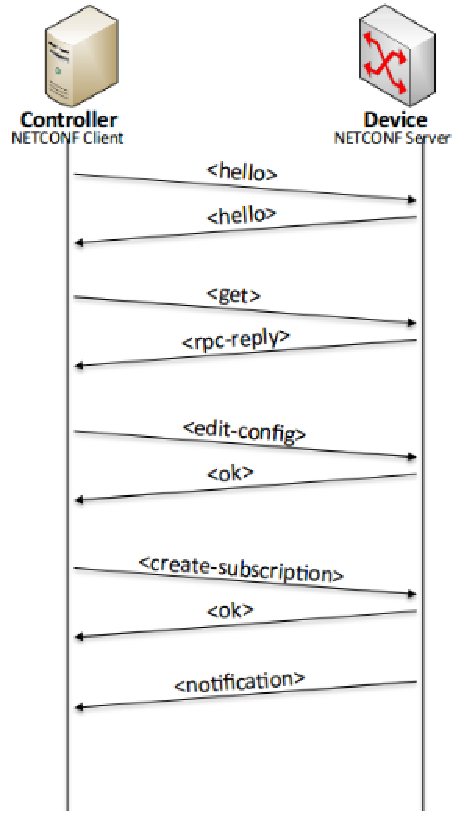
\includegraphics[scale=0.8]{Figures/netconf_ejemplo.pdf}
	\caption{Ejemplo de comunicación entre cliente y servidor NETCONF.}
	\label{fig:netconf_ejemplo}
  \end{figure}

  \subsection{Lenguaje de Modelado \textit{YANG}}
  Como se mencionó anteriormente, \textit{NETCONF} utiliza \textit{YANG} para modelar los datos de estado, los datos de configuración, las \textit{RPC} y las notificaciones. \textit{Yet Another Next Generation} es un lenguaje de modelado de datos desarrollado y estandarizado en la \textit{RFC 6020} por la \textit{IETF} en el año 2010 \parencite{yangrfc}. Si bien existen en la actualidad lenguajes de modelado como \textit{XML Schema}, \textit{SMI}, \textit{UML}, entre otros, la ventaja que presenta \textit{YANG} frente a los demás es que es un lenguaje de modelado específico para gestión de la configuración de red.

  \subsubsection{Conceptos del Lenguaje}
  \textit{YANG} define, en la sección 4.1 de la \textit{RFC 6020}, las funcionalidades de la red separando los datos de estado de los datos de configuración y presentando la información como una estructura de árbol jerárquica. Consiste en una serie de declaraciones y tipos que pueden ser usadas para definir los datos que se quieren modelar. Estas definiciones son contenidas en un módulo y describen qué tipo de datos admite una variable. A su vez, un módulo puede heredar definiciones de otro módulo.

  \subsubsection{Módulos y submódulos}
  Definen una estructura para el modelado de datos. Tienen un diseño predefinido que se debe seguir. Este diseño comienza con un encabezado, siguiendo de las declaraciones que contenga el módulo y por último las revisiones y comentarios respecto al mismo. 
  \\

  Se define el nombre del módulo, un prefijo para identificarlo, las dependencias, información de contacto al autor, descripción y revisiones. La declaración \textit{“include”} permite referenciar material que se describe en un submódulo, mientras que la declaración \textit{“import”} permite referenciar material que se encuentra descrito en un módulo externo. La estructura básica de un módulo puede verse en la figura \ref{fig:estructura_modulo}.

  \begin{figure}[htbp]
	\centering
	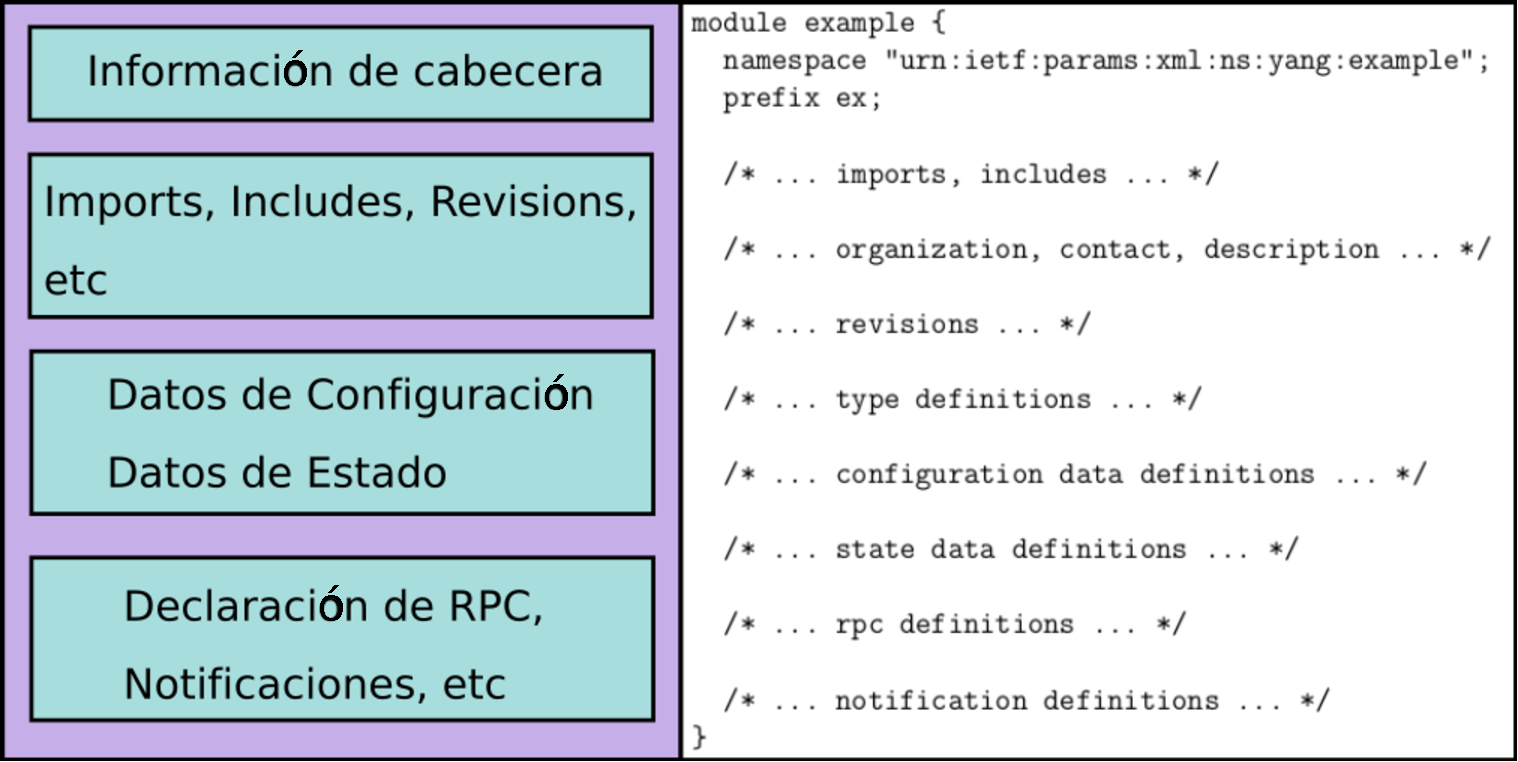
\includegraphics[scale=0.6]{Figures/estructura_modulo.pdf}
	\caption{Estructura de un módulo \textit{YANG}.}
	\label{fig:estructura_modulo}
  \end{figure}

  \subsubsection{Declaraciones y Definiciones de Datos}
  A continuación, se describen algunas sentencias que podría contener un módulo \textit{YANG}. Cada sentencia contiene la definición del tipo de dato y puede contener además algún valor para ese tipo de dato. Siempre representan a datos de configuración o datos de estado, realizando dicha distinción con la sentencia llamada \textit{“config“}.  

  \begin{itemize}
	\item \textbf{\textit{leaf}:} contiene un dato simple como un entero o un \textit{string}. Admite exactamente un valor para un tipo de dato particular y opcionalmente puede incluir una descripción. 
	\item \textbf{\textit{leaf-list}:} describe una secuencia de datos tipo \textit{leaf}. Cada \textit{leaf} admitirá un solo valor para el tipo de dato que especifique el \textit{leaf-list}.
	\item \textbf{\textit{container}:} es utilizado para agrupar datos lógicamente relacionados. Un \textit{container} no admite un valor, pero sí admite cualquier número de tipos de datos como \textit{leaf}, \textit{leaf-list}, \textit{container} o \textit{list}.
	\item \textbf{\textit{list}:} define una secuencia de tipo de datos donde cada tipo de dato es única, identificado por la sentencia \textit{key}. Puede contener múltiples identificadores \textit{key} y cualquier cantidad de tipo de datos \textit{leaf}, \textit{leaf-list}, \textit{container}, etc.
	\item \textbf{\textit{choices - cases}:} no describen algún tipo de dato, más bien ofrecen ramificaciones condicionales en la estructura del módulo. La sentencia \textit{choice} es una condición que asegura que, como máximo, se cumplira una de las declaraciones dadas por case.
\end{itemize}

Las declaraciones y sentencias descritas anteriormente pueden ser utilizadas en conjunto para poder formar una estructura de datos tipo árbol más compleja.
Además, \textit{YANG} admite la reutilización de sentencias mediante las declaraciones \textit{include} e \textit{import} reduciendo así los posibles errores en el modelado de datos.

\subsubsection{Identificador de instancia }
Cada dato en \textit{YANG}, así como el propio módulo, tiene un identificador único de instancia que se puede utilizar para referirse a él. Los identificadores se denominan \textit{namespace}, y admiten un prefijo para poder acortar el nombre. 
\\

Por ejemplo, Bjorklund \parencite{yangsystem}, definió un módulo \textit{YANG} para la administración de interfaces. Dicho modelo tiene una estructura de datos de tres niveles para una interfaz básica. En el nivel superior del modelo se encuentra definido el \textit{container} llamado \textit{“interface”}, seguido de la \textit{list “interface”} que contiene múltiples instancias de una interfaz, identificada por la \textit{key “name”}. Además, cada interfaz tiene una \textit{leaf “enabled”} que describe el estado de la misma. Un ejemplo de identificador para una instancia de \textit{“interface”} llamada \textit{“eth0”} puede verse en la figura \ref{fig:interfaceyang}.

\begin{figure}[htbp]
	\centering
	
\includegraphics[scale=0.9]{Figures/interface-yang.pdf}
	\caption{Ejemplo de identificador de instancia en \textit{YANG}.}
	\label{fig:interfaceyang}
  \end{figure}

  \subsubsection{Funcionalidades}
  \textit{YANG} ofrece características especiales que lo distinguen de un documento \textit{JSON}, permitiéndole describir de forma eficiente las funcionalidades de la red. Estas características incluyen la validación de modelos, una forma estandarizada de extender a los módulos y compatibilidad entre las diferentes revisiones de los mismos. En esta sección, se analizaron las principales funcionalidades ofrecidas por \textit{YANG}.

  \begin{itemize}
	\item \textbf{Validación:} una de las características más importantes de \textit{YANG} es la posibilidad de validar automáticamente todos los datos descritos en el modelo. Resulta importante ya que la validación de los datos es una tarea difícil. Dicha afirmación está respaldada por el hecho de que introducir datos erróneos y tomarlos como válidos, está catalogada como la principal amenaza de seguridad según \textit{OWASP} \parencite{owasp}, organización sin ánimo de lucro a nivel mundial dedicada a mejorar la seguridad de las aplicaciones y del software en general. Cada dato introducido en el modelo \textit{YANG} puede ser validado semánticamente y sintácticamente. La validación de sintaxis es automática y garantiza que el dato contenga una secuencia de bytes válido, puesto que cada dato en el modelo tiene asociado un \textit{type} (string, int, uint, etc). Por otra parte, la validación semántica resulta más compleja y puede ser usada para describir dependencias entre datos. \textit{YANG} también admite sentencias como \textit{“when”} o \textit{“must”} que pueden ser usadas para evaluar condicionalmente un dato.  
	\item \textbf{Compatibilidad:} cada módulo admite la indicación de una revisión, esto permite a \textit{YANG} distinguir las versiones soportadas y adaptarse a la situación cuando la misma no es soportada. También, se describen reglas de actualización en los módulos que deben respetarse para mantener compatibilidad entre los modelos de datos anteriores. Por ejemplo, cualquier cambio en un módulo debe indicar una revisión en la cabecera, tanto el nombre del mismo como el namespace debe mantenerse, como así también las definiciones de datos obsoletas, lo que permite compatibilidad con modelos de datos anteriores. Esta característica permite a los módulos evolucionar con el paso del tiempo, sin romper aplicaciones existentes con versiones anteriores.
	\item \textbf{Extensión:} permite extender las funcionalidades de los módulos con nuevas definiciones de datos. Existen muchas razones por las cuales utilizar la extensión en \textit{YANG}, como por ejemplo, desarrollar un nuevo módulo a partir de uno existente o con el fin de reducir errores reutilizando un módulo funcional. Una ventaja importante que tiene utilizar la extensión, es que al agregar nueva información en un módulo, se mantiene compatibilidad con el heredado.
\end{itemize}

\subsection{Redes Ópticas de Transporte}
La explosión del tráfico digital provocado por los nuevos enfoques como \textit{Big Data} o el \textit{Streaming}, y los requerimientos de los usuarios donde existe un constante crecimiento de aplicaciones con alta demanda de ancho de banda, requieren de una nueva tecnología de transporte que pueda ocuparse de los patrones de tráfico y los contenidos de datos modernos. Para ello, se han realizados numerosos avances en los últimos años referente al plano de control y el plano de datos de las redes ópticas \parencite{redesopticas}, surgiendo protocolos como SONET o OTN. En esta sección, se analiza las redes ópticas, utilizadas para el transporte de los datos como así también los dispositivos que funcionan sobre dichas redes. 
\\

Una red de transporte óptica, es un tipo de red de comunicaciones de datos que utiliza la luz como medio de transporte para la información \parencite{redesopticasdef}. A diferencia de las redes basadas en cobre, los pulsos de luz de una red óptica pueden transportarse a una distancia considerable e incluso regenerarse a través de un dispositivo repetidor óptico. Después de que una señal óptica es recibida en su red de destino, la misma se convierte en una señal eléctrica a través de un receptor óptico, para luego ser enviado al nodo de la capa de paquetes. 
\\

Un sistema de comunicaciones ópticas puede incluir diversos dispositivos, como ser:

\begin{itemize}
	\item \textbf{Amplificadores ópticos} 
	\item \textbf{\textit{Switches} ópticos,} encargados de conmutar de un canal a otro.
	\item \textbf{Divisores de luz,} cuya tarea comprende dividir la señal en diferentes caminos de fibra óptica.
	\item \textbf{Fibra óptica,} que cumple de medio de transporte de la información entre los diferentes equipos.
	\item \textbf{\textit{Transponders} y \textit{Muxponders},} encargados de enviar y recibir las señales ópticas por las fibras. Generalmente son caracterizados por el ancho de banda que pueden transportar y la distancia que puede alcanzar la transmisión.
\end{itemize}

\subsubsection{\textit{Transponders} y \textit{Muxponders}}
El \textit{transponder}, es un dispositivo que recibe múltiples señales ópticas a través de sus puertos clientes, dichas señales ópticas pueden tratarse de servicios diferentes como por ejemplo, \textit{Ethernet}, \textit{SONET}, \textit{OTN}, entre otros. Luego, transforma estas señales en flujos de datos eléctricos, las procesa y regenera las mismas para nuevamente convertirlas en señales ópticas compatibles con el estándar \textit{ITU}. De esta forma, realiza la función de recepción, amplificación y reemisión de una señal óptica en un proceso que comúnmente se denomina \textit{optical electrical optical} (OEO) \parencite{transpondermux}.
\\

La figura \ref{fig:transponder} ejemplifica el proceso \textit{OEO} típico de un \textit{transponder}.

\begin{figure}[H]
	\centering
	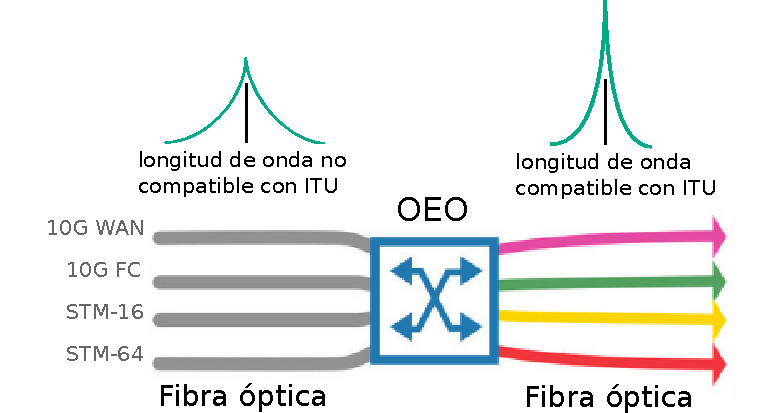
\includegraphics[scale=0.9]{Figures/transponder.pdf}
	\caption{Funcionamiento básico de un \textit{transponder}.}
	\label{fig:transponder}
  \end{figure}

  Por otra parte, los \textit{muxponders} realizan una función similar a los \textit{transponders}. También incluyen el proceso \textit{OEO}, con la diferencia de que combinan múltiples servicios en una sola longitud de onda que luego se multiplexan en la misma fibra \parencite{transpondermux}. Por lo tanto, en lugar de asignar a cada servicio una longitud de onda dedicada, permite que varios servicios diferentes compartan la misma longitud de onda. Estos dispositivos maximizan la utilización de la fibra y ofrecen soluciones de bajo costo para empresas y transportistas. La figura \ref{fig:muxponder} muestra el comportamiento de un \textit{muxponder}.

  \begin{figure}[htbp]
	\centering
	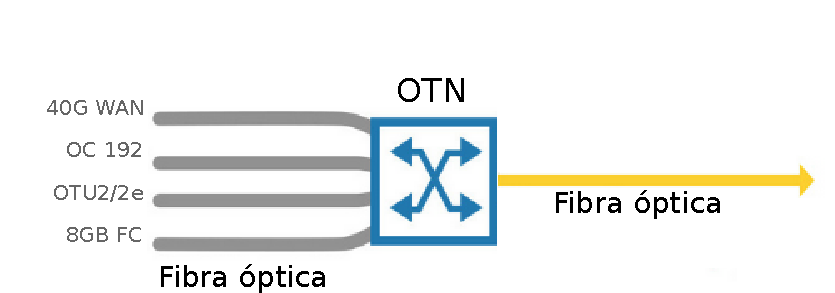
\includegraphics[scale=0.9]{Figures/muxponder.pdf}
	\caption{Funcionamiento básico de un \textit{muxponder}.}
	\label{fig:muxponder}
  \end{figure}

  \subsubsection{Aplicaciones}
  Resulta importante ahora separar la red en dos capas diferentes: la capa de paquetes o de \textit{IP/MPLS}, y la capa óptica o de transporte \parencite{capasredess}. La figura \ref{fig:capasredes} muestra dicha separación.  Los dispositivos mencionados anteriormente se utilizan en la capa de transporte mientras que los \textit{routers} y \textit{switches} convencionales se encuentran en la capa \textit{IP/MPLS}.
  \\

La función que tienen los \textit{muxponders} es la de proveer una conexión lógica entre los diferentes \textit{routers}, quienes podrían estar separados por enormes distancias donde los protocolos como \textit{Ethernet} no proveen un buen servicio de transporte. 
\\

De esta forma, los dispositivos de la capa \textit{IP/MPLS} tienen conocimiento de sus vecinos pero no de la forma en la que se encuentran conectados ni de cómo se está realizando dicha comunicación, mientras que los equipos de la capa óptica esencialmente emparejan a los dispositivos de la capa \textit{IP/MPLS}, pero sin tener conocimiento sobre los diferentes servicios que se prestan. 

\begin{figure}[htbp]
	\centering
	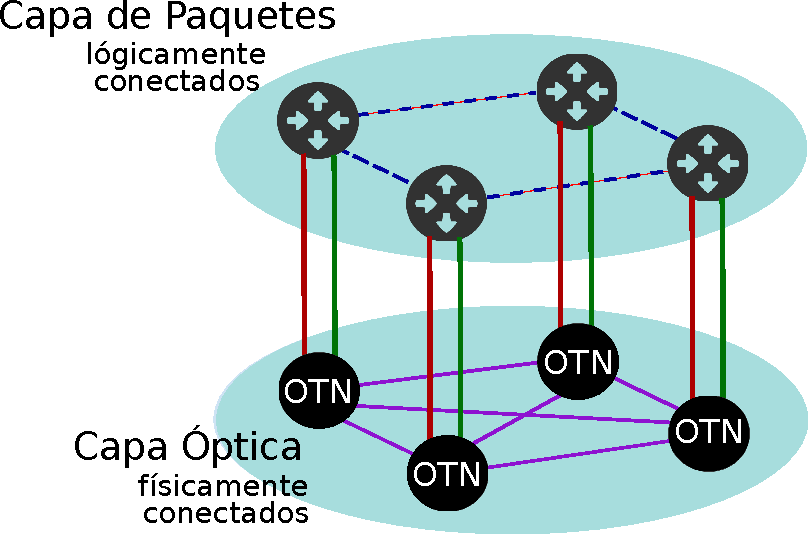
\includegraphics[scale=0.8]{Figures/capasredes.pdf}
	\caption{Separación de la red en capa de paquetes y capa de transporte.}
	\label{fig:capasredes}
  \end{figure}
 % Chapter Template 
% cSpell: words Mininet prototipado parencite enrutamiento includegraphics veth  mininetonf cellcolor Nicira vswitchd interconectar multicapa datapath ovsflow resizebox flowtable netlink OVSDB dpctl ofctl vsctl rowcolor mininetovs
 
\chapter{Análisis de las tecnologías} % Main chapter title

\label{Chapter3} % Change X to a consecutive number; for referencing this chapter elsewhere, use \ref{ChapterX}

Teniendo en cuenta los conceptos revisados en el capítulo anterior, en este se estudiarán las herramientas que permitirán la realización del proyecto. 

En la primera sección, se realizará un análisis del dispositivo utilizado, un \textit{muxponder} óptico coherente de 40GB desarrollado por la institución donde se realizó el proyecto.

Luego, en la segunda sección se examinarán las herramientas de software involucradas. La misma se encuentra dividida en dos partes; la primera detalla el funcionamiento del controlador \textit{SDN} utilizado, \textit{ONOS}; la segunda refiere al estudio de dos agentes \textit{NETCONF}: Sysrepo y Yuma123.


%----------------------------------------------------------------------------------------
%	SECTION 1
%----------------------------------------------------------------------------------------

\section{Herramientas de Hardware}

Para cumplir con el objetivo del proyecto, será de suma importancia conocer las bondades y las limitaciones del equipo con el que se cuenta. Así, esta sección comprende el estudio de uno de los dispositivos mencionados en el capítulo anterior, un \textit{muxponder}. Concretamente, se analizarán aspectos técnicos relacionados tanto al hardware como al software de un \textit{muxponder} de 40GB. El interés del análisis resulta en que es en este dispositivo en donde se integrará el protocolo de gestión \textit{NETCONF}.

\subsection{\textit{Muxponder} 40GB}

El muxponder con el que se cuenta es capaz de realizar una transmisión óptica de 40GB/s sobre una señal de línea \textit{OTU3}. La misma es lograda cumpliendo el estándar \textit{ITU-T G.709} \parencite{itu7}, utilizando una modulación coherente \textit{DP-QPSK} o \textit{DP-DQPSK}.
Dispone de cuatro clientes ópticos asíncronos totalmente independientes de 10GB/s cada uno, a través de módulos ópticos  \textit{XFP} removibles. Las longitudes de ondas soportadas para los clientes son 850/1310/1550 nm y admite los tipos de cliente \textit{10GB Ethernet LAN/WAN, OTU2} y \textit{OTU2e}.
\\

Además, incorpora el mecanismo de corrección de errores \textit{FEC} para todas las señales, tanto para clientes como para línea. Mediante el mismo, el \textit{muxponder} es capaz de realizar correcciones sin necesidad de retransmitir la información.
\\

En términos de potencia, alcanza típicamente los 93 Watts. También, el dispositivo puede alcanzar una distancia de hasta 2000Km.
\\

Las interfaces de conexión soportadas para realizar configuración y monitoreo en el dispositivo son: 
\begin{itemize}
	\item 2 puertos \textit{Ethernet}.
	\item 1 puerto serial \textit{RS232}.
	\item 1 puerto \textit{USB} 2.0.
\end{itemize}

En la figura \ref{fig:mux40} se puede observar en el panel frontal del equipo con las diferentes interfaces mencionadas anteriormente.


\begin{figure}[H]
	\centering
	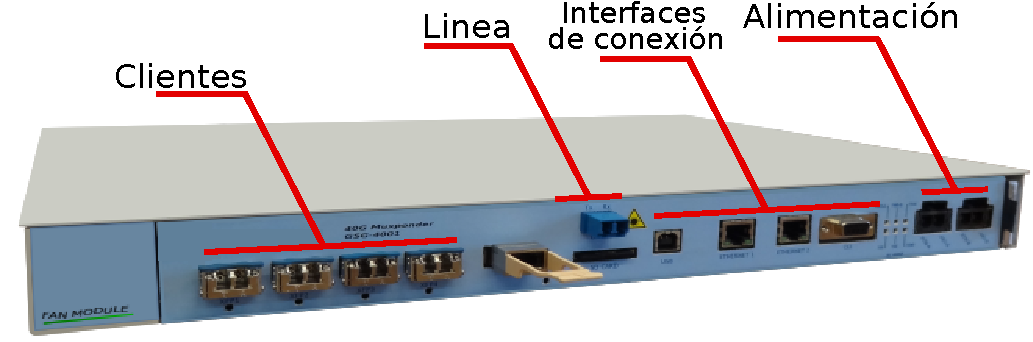
\includegraphics[scale=0.7]{Figures/mux40.pdf}
	\caption{Vista del panel frontal del \textit{muxponder} de 40GB utilizado.}
	\label{fig:mux40}
  \end{figure}

  Por otra parte, el \textit{muxponder} de 40GB integra un total de 128MB de memoria \textit{RAM} y 512MB de almacenamiento, con capacidad de extender esta última mediante una tarjeta \textit{SD}. Además, cuenta con un sistema operativo Linux \textit{'Buildroot'}, el cual ocupa gran parte de estos recursos mencionados, dejando libre para las aplicaciones de usuario un total de 100MB de \textit{RAM} y 270MB de almacenamiento.

El hecho de que presente dicho sistema operativo resulta en una ventaja por varios motivos, en primer lugar porque el mismo es un entorno conocido por el alumno, donde además podrán ejecutarse en él la mayoría de las aplicaciones \textit{UNIX} típicas. En segundo lugar, el sistema operativo integra librerías y herramientas que facilitaran el desarrollo del proyecto, como por ejemplo la librería \textit{SSH}, necesaria por el protocolo \textit{NETCONF}.
\\

Por último, el procesador que incorpora es un \textit{NIOS II} de primera generación fabricado por \textit{Intel} \parencite{intelaltera}. El mismo funciona a 125 Mhz y se encuentra integrado en una \textit{FPGA}. Es importante destacar que la arquitectura de este procesador no es una arquitectura típica de una máquina de propósito general (por ejemplo \texttt{x86\_64}), por lo tanto, las distintas aplicaciones que se ejecuten en esta plataforma deberán estar compiladas específicamente para la arquitectura \textit{NIOS}. 

Además, debido a las capacidades de la memoria primaria y secundaria del equipo, resulta imposible realizar la compilación de las aplicaciones sobre el mismo. Por lo tanto, se deberá realizar lo que se conoce como compilación cruzada, que consiste en preparar un sistema huésped (donde generalmente dicho sistema cuenta con mayores recursos y capacidades) para generar todos los binarios y librerías que requiere el dispositivo objetivo donde finalmente se ejecutarán las aplicaciones.

\newpage

\subsection{Componentes del \textit{muxponder}}

Los componentes más significativos del dispositivo se listan a continuación:

\begin{itemize}
	\item Módulo de 40GB.
	\item Los 4 puertos clientes (XFP).
	\item Unidad de ventilación.
	\item Chip cortina.
	\item Unidad de alimentación.
	\item Interfaces de control.
	\item \textit{FPGA}, con el procesador \textit{NIOS II} instanciado.
\end{itemize}


Además, se presenta en la figura \ref{fig:diagramabloque} un diagrama en bloques del \textit{muxponder}, donde se pueden observar los principales componentes que conforman el mismo.

\begin{figure}[H]
	\centering
	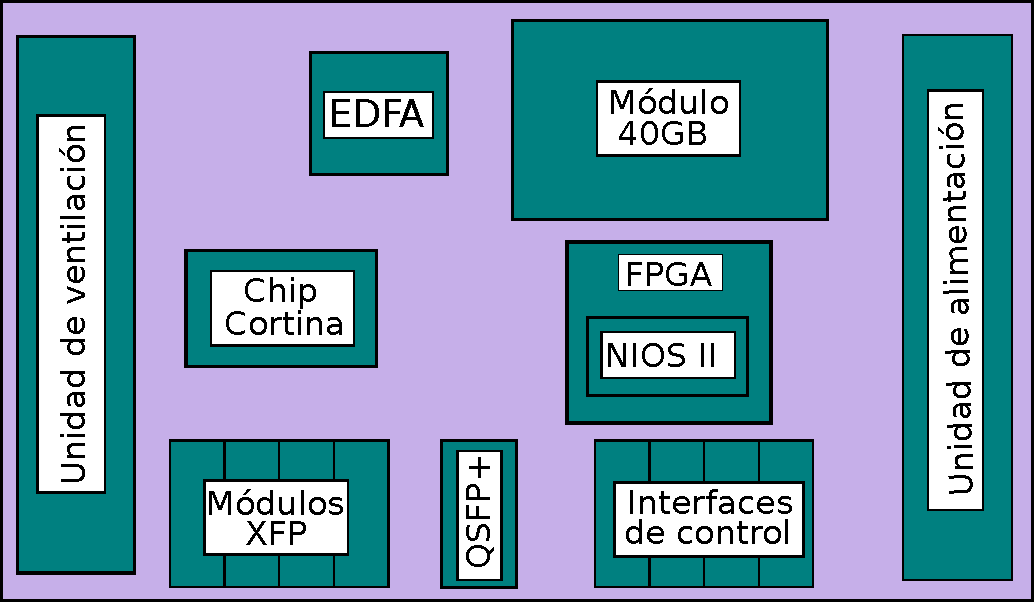
\includegraphics[scale=0.60]{Figures/diagramabloquesmxp.pdf}
	\caption{Diagrama en bloques del \textit{muxponder} de 40GB.}
	\label{fig:diagramabloque}
  \end{figure}

Por otra parte, una vista de la circuitería del equipo se puede observar en la figura \ref{fig:diagramabloquemxp}.

\begin{figure}[H]
	\centering
	\includegraphics[scale=0.060]{Figures/bloquemxpfisico.pdf}
	\caption{Vista de la circuitería del \textit{muxponder} de 40GB.}
	\label{fig:diagramabloquemxp}
  \end{figure}

\subsection{Aplicaciones integradas en el dispositivo}

Será importante explicar la utilidad de dos binarios que incorporan los \textit{muxponders} de 40GB: 'monitor' y 'muxponder'. 

\begin{itemize}
	\item \textbf{'monitor'}: aplicación que permite mostrar información del dispositivo a través de la \textit{CLI}. Con el fin de agrupar y ordenar los datos relacionados, los mismos se encuentran divididos en secciones. Por ejemplo, se tiene una sección dedicada a mostrar la temperatura de los diferentes módulos, las alarmas relacionadas a la transmisión y recepción, otra sección referida a la presencia de los módulos XFP del equipo, entre otros. De esta forma, el administrador podría conocer el estado del dispositivo ejecutando dicha aplicación y observando la salida producida en pantalla.
	
	Por otra parte, el equipo utiliza el método de comunicación entre procesos llamado memoria compartida. El mismo consiste en una región de memoria donde se permite que otras aplicaciones puedan, por ejemplo, leer información. Así, la aplicación 'monitor' también es la encargada de actualizar en memoria compartida los valores de todos los datos a monitorear, permitiendo que otras aplicaciones puedan leer y acceder a dicha información.
	
	A continuación, se muestra en la figura \ref{fig:monitor} una porción de la salida en pantalla producida por la aplicación 'monitor'. En ella se puede observar la sección relacionada a los módulos XFP del \textit{muxponder}.
	
	\begin{figure}[H]
		\centering
		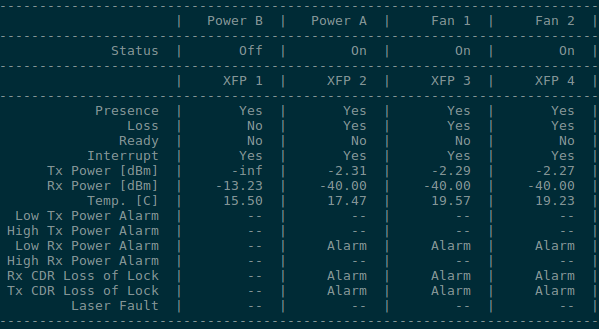
\includegraphics[scale=0.77]{Figures/monitorapp.png}
		\caption{Sección XFP de la aplicación ’monitor’.}
		\label{fig:monitor}
	  \end{figure}

	\item \textbf{'muxponder'}: Por otra parte, la aplicación 'muxponder' es utilizada por el administrador para poder configurar el dispositivo mediante ciertos parámetros que son especificados haciendo uso de la \textit{CLI} del equipo. Por ejemplo, con esta aplicación el administrador podría cambiar la configuración de un \textit{muxponder} que tiene un tipo de tráfico $otu2$ por un tipo de tráfico $xge$ a través de la CLI, tal como se muestra en la figura \ref{fig:mxpapp}.

	\begin{figure}[H]
	  \centering
	  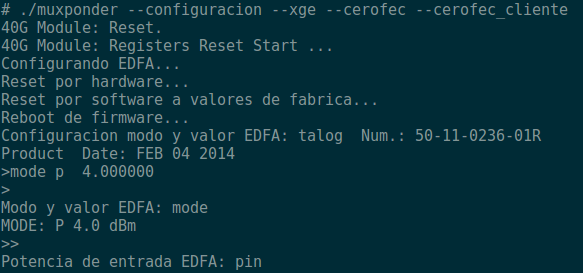
\includegraphics[scale=0.63]{Figures/muxponderapp.png}
	  \caption{Configuración mediante la aplicación ’\textit{muxponder}’.}
	  \label{fig:mxpapp}
	\end{figure}
\end{itemize}



  

%----------------------------------------------------------------------------------------
%	SECTION 2
%----------------------------------------------------------------------------------------



\section{Herramientas de Software}

Además del estudio del hardware utilizado, resulta de interés realizar un análisis de los componentes de software que conforman el proyecto. Para ello, la primer parte de esta sección estará dedicada a estudiar el controlador \textit{SDN} empleado, mientras que en la segunda parte se analizarán dos agentes \textit{NETCONF} disponibles de código abierto.

\subsection{Controlador \textit{ONOS}}
El controlador \textit{ONOS}, desarrollado y mantenido por la \textit{ONF} \parencite{onff}, es uno de los controladores abiertos más comunes en la industria, donde destacan miembros como Google, Intel, \texttt{AT\&T}, Samsung, entre una numerosa lista \parencite{onffmembers}. Está diseñado específicamente para los proveedores de servicios, donde sus principales objetivos son la escalabilidad y el alto rendimiento \parencite{onffwhite}.

Las licencias compatibles con \textit{ONOS} son \textit{Apache} 2.0, \textit{MIT} y \textit{BSD} \parencite{onfflic}. El hecho de que sea un proyecto \textit{open-source}, supone ventajas como ser interoperabilidad, personalización, flexibilidad e independencia del fabricante. 

Antes de detallar cómo funciona y realizar un análisis de su arquitectura, es importante explicar el problema que enfrentan los controladores \textit{SDN} para poder entender las ventajas que supone el mismo. 
\\

Debido al crecimiento del consumo de tráfico en las redes y la demanda del ancho de banda en alza, es necesario para los proveedores de servicio que el rendimiento y la escalabilidad de sus redes no se vean afectadas por estos motivos. De este modo, los controladores \textit{SDN} deben poseer tres atributos claves: escalabilidad, rendimiento y alta disponibilidad \parencite{sdnproblema}.

\begin{itemize}
	\item \textbf{Escalabilidad}: como se explicó en el capítulo anterior, \textit{SDN} introduce una autoridad de control centralizada. La misma, debe ser capaz de escalar de igual forma que las funcionalidades de la red, manteniendo su rendimiento.
	\item \textbf{Alta disponibilidad}: el plano de control que se encuentra centralizado en el controlador, juega ahora un papel crítico. Esto es así ya que si el mismo se encuentra sobrecargado o deja de estar disponible por alguna razón, la funcionalidad de la red se vería afectada. Por lo tanto, las diferentes soluciones \textit{SDN} deberán brindar disponibilidad ininterrumpida del controlador.
	\item \textbf{Rendimiento}: el controlador también tiene que ser capaz de proveer mecanismos para adaptarse dinámicamente ante las fluctuaciones en la carga del tráfico y la congestión de la red, evitando que el rendimiento del mismo se vea afectado. 
\end{itemize}

\subsubsection{Arquitectura del controlador}
Las características más importantes de la arquitectura presentada por \textit{ONOS} \parencite{onffwhite} se detallan a continuación:

\begin{itemize}
	\item \textbf{Núcleo distribuido}: la solución que propone \textit{ONOS} para proveer escalabilidad, alto rendimiento y disponibilidad, se basa en un núcleo distribuido por los diferentes nodos que conforman un \textit{cluster}, lo que implica la posibilidad de soportar enormes cantidades de dispositivos de red. Esto último es así ya que \textit{ONOS} permite la incorporación dinámica de nuevos nodos, con lo que la carga del controlador podría distribuirse entre ellos de forma adaptativa.
	
	La figura \ref{fig:onosdistribuido} ejemplifica dicha distribución. El hecho de agregar esta redundancia implica una mayor disponibilidad del controlador. A su vez, permite realizar un balanceo de carga, lo que implica mayor rendimiento y escalabilidad.


	\item \textbf{Abstracción \textit{Northbound}}: el plano aplicación, explicado en el capítulo anterior, se comunica con \textit{ONOS} a través de una interfaz brindada por el controlador. El mismo, brinda a las aplicaciones gráficos y estadísticas de la red como así también aplicaciones basadas en \textit{intents} para facilitar el control, administración y configuración de los equipos.
	\item \textbf{Abstracción \textit{Southbound}}: de forma similar, el controlador ofrece una interfaz para comunicarse con el plano de datos. Cabe destacar que si bien \textit{ONOS} basa su funcionamiento en el protocolo \textit{OpenFlow}, también brinda soporte a otros como \textit{NETCONF}, \textit{REST}, \textit{SNMP}, etc, con el fin de mantener compatibilidad con dispositivos más antiguos.
	
	Una aproximación más detallada de la arquitectura que presenta \textit{ONOS} puede verse en la figura \ref{fig:onosarch}. En la misma, se observan las interfaces mencionadas anteriormente junto a una serie de componentes que pertenecen a la interfaz \textit{Southbound}. Estos componentes se analizarán más adelante. 

	\item \textbf{Modularidad}: el controlador se encuentra desarrollado en \textit{Java}, y mediante el \textit{framework} OSGi, obtiene las características de una arquitectura modular. De esta forma, se provee a los desarrolladores facilidad para brindar actualizaciones a sus aplicaciones, poder monitorearlas, realizar depuración y mantenimiento.  
\end{itemize}

\begin{figure}[H]
	\centering
	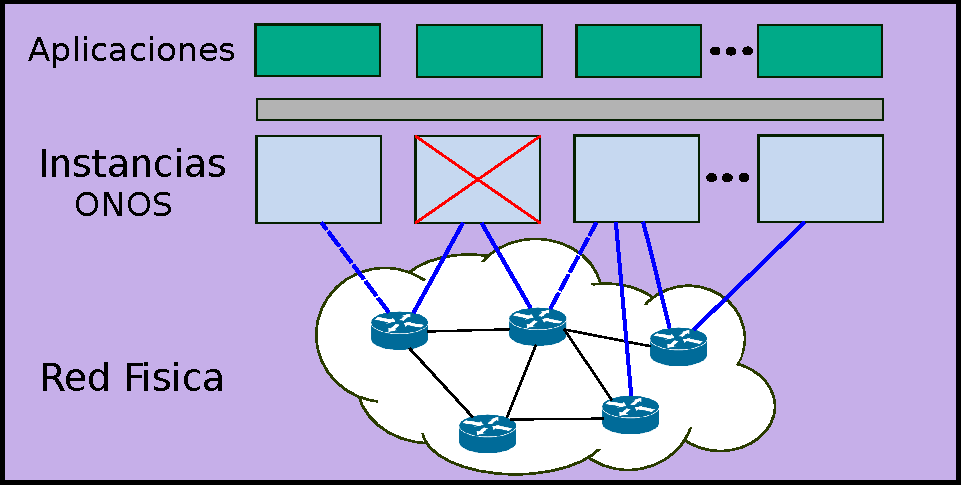
\includegraphics[scale=0.7]{Figures/onosarch.pdf}
	\caption{Arquitectura distribuida de \textit{ONOS}.}
	\label{fig:onosdistribuido}
  \end{figure}

  

  \begin{figure}[H]
	\centering
	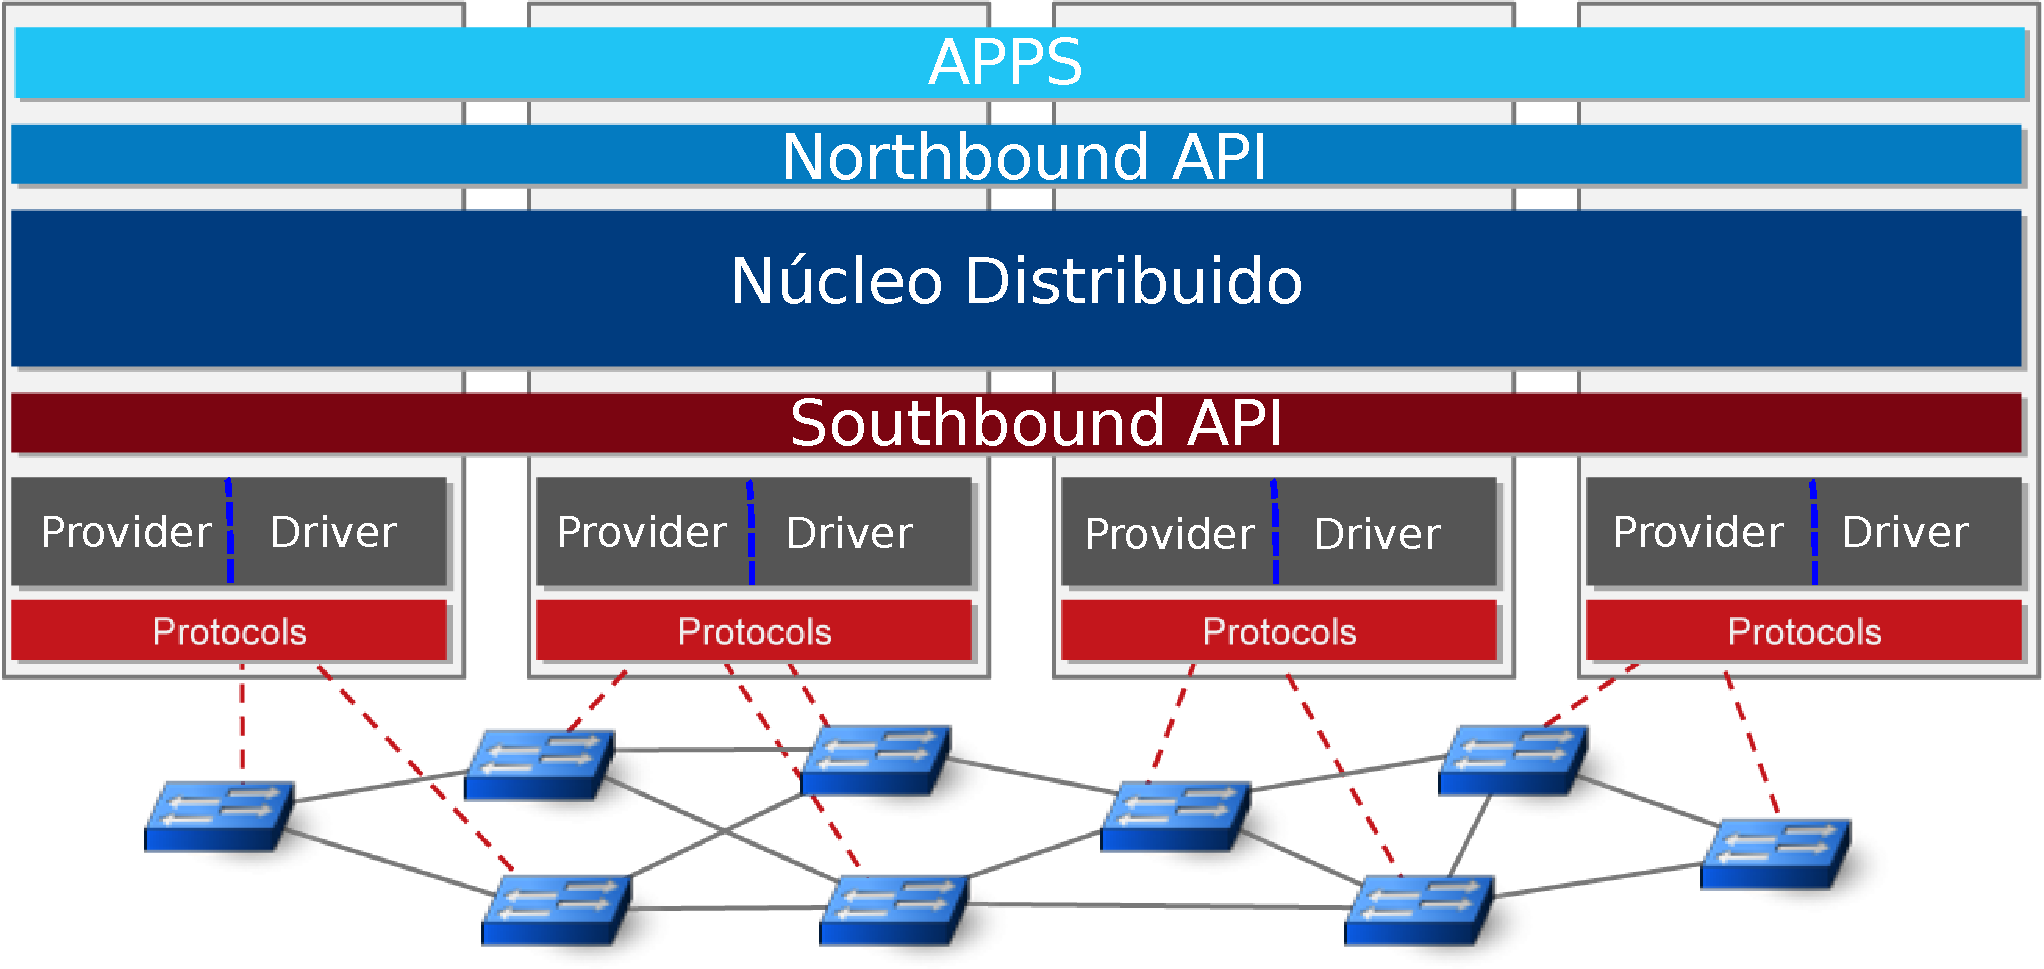
\includegraphics[scale=0.40]{Figures/corecompleto.pdf}
	\caption{Arquitectura completa del controlador \textit{ONOS}.}
	\label{fig:onosarch}
  \end{figure}

  \subsubsection{Interfaz \textit{Southbound} en \textit{ONOS}}
  Tal como se explicó anteriormente, el objetivo del proyecto es gestionar la configuración de un \textit{muxponder} de 40GB a través del protocolo \textit{NETCONF}. 
  
  Para ello, se procede a explicar con más detalle la interfaz \textit{Southbound} de \textit{ONOS}. La misma, se encuentra dividida en una serie de componentes que se detallan a continuación:

  \begin{itemize}
	\item \textbf{\textit{Providers}}: son aplicaciones independientes que residen en el núcleo de \textit{ONOS} y que pueden activarse o desactivarse dinámicamente en tiempo de ejecución. El propósito principal de esta capa es abstraer al \textit{core} las complejidades de los protocolos, brindando interfaces de las operaciones típicas y generales de los mismos. Un ejemplo de un \textit{provider} en \textit{ONOS} es el llamado \textit{'NetconfAlarmProvider'}, encargado de transformar cada notificación de los dispositivos en una alarma registrada en \textit{ONOS}.
	\item \textbf{\textit{Protocols}}: es la capa de más bajo nivel en la interfaz \textit{Southbound} y es la única que tiene contacto directo con los dispositivos conectados al controlador. Aquí se implementan los diferentes protocolos necesarios para la comunicación como ser \textit{NETCONF}, \textit{REST}, \textit{SNMP}, etc. Comúnmente se utilizan librerías de terceros como \textit{openflowj, snmp4j, thrift}, entre otras.
	\item \textbf{\textit{Drivers}}: al igual que los \textit{providers}, los \textit{drivers} pueden cargarse dinámicamente al núcleo del controlador y proveen mecanismos para comunicarse con los diferentes dispositivos a través de algún protocolo. La diferencia principal con los \textit{providers}, es que aquí no se implementan generalidades de los protocolos, sino comportamientos específicos de los dispositivos. Además, sirve de interfaz entre las aplicaciones que se encuentran en la capa \textit{Northbound} y los diferentes equipos de red. El propósito principal de este subsistema es el de aislar el código específico del dispositivo, de tal manera de que el mismo no se extienda por el resto del núcleo de \textit{ONOS}. Dado que dicho código será necesario para cualquier futuro previsible, este subsistema proporciona medios para contenerlo y permitir que otros subsistemas (por ejemplo, la capa de aplicación) interactúen con él a través de abstracciones independientes del protocolo y del dispositivo. Por último, presenta una ventaja para los desarrolladores de hardware dado que al ser un componente modular, permite la herencia de funcionalidades de otros \textit{drivers} con el fin de compartir características con una familia de dispositivos en común.
\end{itemize}

La figura \ref{fig:onosarchsouth} esclarece la participación que tiene cada componente tanto con el \textit{core} como con el dispositivo.

\begin{figure}[H]
	\centering
	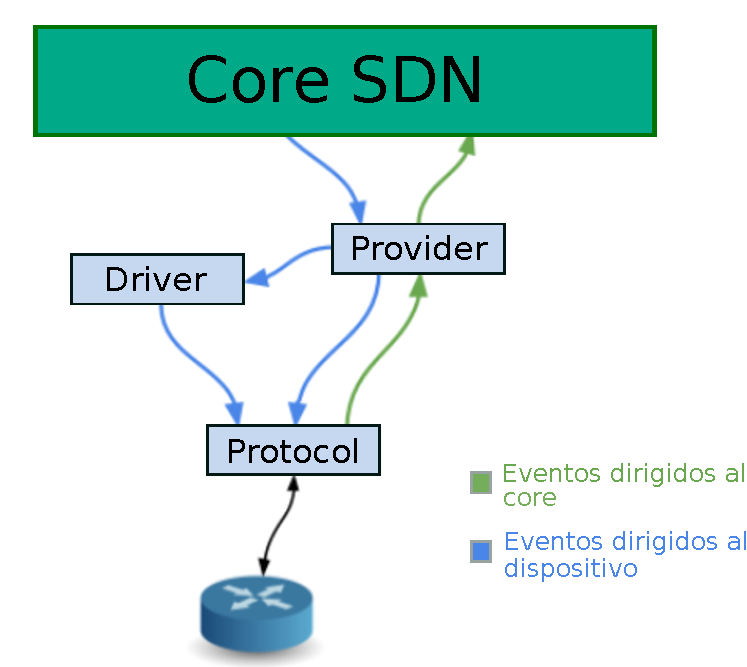
\includegraphics[scale=0.67]{Figures/southboundonos.pdf}
	\caption{Interfaz \textit{Southbound} en \textit{ONOS}.}
	\label{fig:onosarchsouth}
  \end{figure}

  \subsubsection{Justificación de la elección del controlador}

En la actualidad, existe una diversidad de controladores \textit{SDN}, como ser \textit{Ryu} (\textit{Python}), \textit{Floodlight} (\textit{Java}), \textit{POX} (\textit{Python}), e incluso implementaciones propietarias. 

Se destaca \textit{OpenDaylight} (\textit{Java}), un controlador abierto que soporta una gran lista de protocolos y que, según \parencite{book_SDN_a_c_a}, junto a \textit{ONOS} es uno de los controladores más utilizados en la industria.

La razón determinante por la cual se optó por \textit{ONOS} como controlador \textit{SDN} radica en que el mismo cuenta con una documentación más clara y organizada. Además, se poseía experiencia previa trabajando con dicho controlador. Todo esto facilitó la curva de aprendizaje de las distintas herramientas, donde se pudo tener una rápida interacción con el controlador dada su facilidad de instalación y puesta en marcha.

Otro motivo reside en que las redes de los proveedores de servicio son complejas y multicapas, donde se requiere una separación clara de la capa de paquetes y de la capa de transporte, tal como se vió en el capítulo anterior. \textit{ONOS}, ha logrado brindar soporte a las redes ópticas según lo demuestra el caso de uso aquí descripto \parencite{onffwhite}.

\subsection{Análisis de agentes \textit{NETCONF}}

Con el fin de poder gestionar la configuración del \textit{muxponder} de 40GB a través de \textit{NETCONF}, se estudiará en esta sección dos implementaciones del protocolo: Sysrepo y Yuma123. 

Las mismas son \textit{open-source}, lo que facilita el estudio y comprensión de los agentes. Finalmente, se justificará la elección de Yuma123 como servidor \textit{NETCONF} para el proyecto.

\subsubsection{Sysrepo}
El proyecto Sysrepo proporciona las funcionalidades de una base de datos lógica a las diferentes aplicaciones Unix-Linux. De esta forma, las aplicaciones pueden gestionar sus datos de configuración y de estado utilizando \textit{YANG} como modelado de datos, a través de las \textit{API’s} e interfaces que expone Sysrepo \parencite{sysrepogit}. Así, la implementación garantiza mediante YANG la consistencia de los datos y la correctitud de los mismos. 

A su vez, Sysrepo integra \textit{Netopeer2} \parencite{netopeergit} como agente \textit{NETCONF}. \textit{Netopeer2} es la evolución del proyecto Netopeer \parencite{netopeergit1} (discontinuado) y ofrece tanto un cliente como un servidor \textit{NETCONF}.
\\

Sysrepo fue la primera implementación del protocolo instalada y manipulada en una máquina de propósito general. Tiene la ventaja de contar con una gran documentación, como así también una variedad de ejemplos y casos de usos. Además, otra ventaja que presenta es que el hecho de que Sysrepo exponga \textit{API’s} implica una posibilidad de adaptar cualquier aplicación Unix existente al protocolo \textit{NETCONF}, sin mayores cambios.  

\subsubsection{Yuma123}
En el 2011, el proyecto \textit{open-source} YUMA, también conocido como OpenYUMA, sufrió un cambio en su licencia donde esta dejó de ser \textit{BSD}. A partir de entonces, el proyecto tuvo dos ramificaciones: YumaPro \parencite{yumapro}, ahora perteneciente a YumaWorks, y Yuma123, su versión \textit{open-source}. 

Yuma123 nace a partir de la última \textit{release} \textit{BSD} del proyecto OpenYUMA, con el fin de continuar con el soporte de dicha implementación mientras se mantiene la licencia \textit{BSD}. Al igual que Sysrepo, ofrece tanto un cliente (yangcli) como un servidor (netconfd) \textit{NETCONF}. La diferencia con la implementación anterior es que aquí no se exponen \textit{API’s} a las aplicaciones, sino que las mismas son directamente compiladas como librerias \textit{SIL} y son dependientes de Yuma123.
\\

Según la documentación \parencite{yuma123}, se agregaron las siguientes funcionalidades con respecto a la versión original de OpenYUMA:

\begin{itemize}
	\item Un sistema de compilación más eficiente, basado en las herramientas \textit{autoconf} y \textit{automake}.
	\item Se han corregidos \textit{bugs} críticos reportados en OpenYUMA.
	\item Soporte de las nuevas funcionalidades del protocolo agregadas por la \textit{IETF} (ietf-nacm, ietf-system, etc.). 
\end{itemize}

\subsubsection{Evaluación de las implementaciones}
A la hora de efectuar una comparación entre ambos proyectos, se tendrán en cuenta los siguientes criterios: las diferencias relativas al protocolo \textit{NETCONF}; las herramientas y características extras que brinda cada una; y los recursos que demandan.

\begin{itemize}
	\item \textbf{Diferencias relativas al protocolo \textit{NETCONF}}: Como se detalló en el capítulo anterior, \textit{NETCONF} define una serie de operaciones que no son obligatorias para las diferentes implementaciones del protocolo, sino que son opcionales y las mismas deberán ser explícitamente anunciadas en el mensaje \textit{HELLO} del servidor. Es importante repasar cuáles de estas operaciones admite cada proyecto. 
		
	Tanto Yuma123 \parencite{yuma123features} cómo Sysrepo \parencite{sysrepogit} implementan el estándar \textit{NETCONF} 1.0 y \textit{NETCONF} 1.1, definidos en los \textit{RFC 4741} \parencite{netconfrfc} y \textit{RFC 6241} \parencite{netconfrfcnuevo} respectivamente. 
	
	Sin embargo, mientras que Sysrepo admite el transporte seguro mediante \textit{SSH} y \textit{TLS}, Yuma123 únicamente soporta \textit{SSH}. Esto último, es una ventaja para Sysrepo ya que brinda flexibilidad y personalización al administrador sobre el protocolo de transporte seguro.
	
	Por otra parte, Sysrepo admite únicamente la operación \textit{commit} sobre la base de datos \textit{candidate}, mientras que Yuma123 además de soportar dicha operación también incorpora las capacidades \textit{confirmed-commit} y \textit{validate}, lo que provee a esta última de potentes herramientas para corroborar la correctitud de los datos ingresados y a su vez restaurar la funcionalidad de la red en caso de ingresar una configuración incorrecta.
	
	Para finalizar, cabe destacar que ambos proyectos soportan las bases de datos \textit{startup} y \textit{candidate}.

	\item \textbf{Herramientas y características extras al protocolo}: Ambas implementaciones integran tanto un cliente como un servidor \textit{NETCONF}. Sin embargo, cada una incorpora una serie de herramientas que resulta de importancia mencionarlas. 
	\newpage
	\begin{itemize}
		\item \textbf{Sysrepo}
		\begin{itemize}
			\item sysrepoctl: aplicación que permite administrar los módulos \textit{YANG} desde una \textit{CLI}. Brinda opciones para instalar, eliminar y listar los módulos que tiene activo el servidor.
			\item sysrepocfg: utilidad para exportar o importar datos de configuración de las diferentes bases de datos. De esta forma se podría editar, por ejemplo, el contenido de la base de datos \textit{startup} desde un navegador \textit{WEB} o editor de texto cualquiera, sin que sea necesario utilizar el protocolo \textit{NETCONF} para dicho propósito.
		\end{itemize}
		\item \textbf{Yuma123}
		\begin{itemize}
			\item yangdiff: herramienta que permite comparar dos revisiones de un mismo módulo \textit{YANG}. El nivel de detalle con el cual se exponen las diferencias puede ajustarse hasta con tres niveles de reporte. Además, puede generar de forma automática la declaración \textit{'revision'} del módulo con detalles de los cambios.
			\item yangdump: posibilita validar módulos \textit{YANG} y convertirlos a otros formatos. De esta forma, mediante un módulo \textit{YANG} la herramienta genera el esqueleto del código \textit{SIL} (lenguaje \textit{C}) que necesita para relacionar la instrumentación del dispositivo con el modelado de los datos.
		\end{itemize}
	\end{itemize}

	Para finalizar el análisis de este criterio, se menciona que ambas implementaciones permiten parametrizar opciones en el servidor \textit{NETCONF}, como por ejemplo el número máximo de sesiones admitidas, el tiempo de espera para una respuesta \textit{RPC} y el tiempo de espera de una sesión inactiva antes de finalizarla. Además, anteriormente se mencionó que mientras Sysrepo expone \textit{API’s} a las diferentes aplicaciones Unix, Yuma123 las integra como librerías \textit{SIL} dependientes de la implementación. Esto último es una ventaja para Sysrepo, ya que tanto Sysrepo como la aplicación funcionarían como procesos diferentes que se comunican mediante interfaces, donde la falla de uno de estos procesos no necesariamente involucra el bloqueo completo del otro. Esto último no sucede en el caso de Yuma123, donde es el servidor quien realiza las llamadas a las librerías \textit{SIL} previamente compiladas, formando un solo proceso.

	\item \textbf{Demanda de recursos}: Al inicio de este capítulo, se estudiaron las características técnicas del \textit{muxponder} utilizado para este proyecto. Será de suma importancia que las implementaciones mencionadas se adapten a los recursos que dispone el equipo, por lo que se hará foco principal en demanda de la memoria \textit{RAM} y de la memoria de almacenamiento. 
	
	Dicho esto, es importante mencionar que para el siguiente análisis se iniciaron los binarios con la configuración por defecto. Además, los datos obtenidos corresponden a la ejecución de los mismos en una máquina de escritorio, sin realizar algún tipo de optimización en recursos.

	\begin{itemize}
		\item \textbf{Sysrepo}: según la documentación \parencite{sysrepoinstall}, se requiere de una extensa lista de librerías de terceros para poder efectuar la compilación e instalación del proyecto. Teniendo en cuenta dichas librerías necesarias para el funcionamiento de Sysrepo, la implementación demanda un espacio total en memoria secundaria de 250MB. Cabe destacar que en este análisis se incluye no solo el servidor Netopeer2 sino también el cliente, ya que Sysrepo necesita de ambos para funcionar. En el caso de memoria \textit{RAM}, Sysrepo ocupa 270MB.

		\item \textbf{Yuma123}: en este caso, la cantidad de librerías de terceros que requiere el proyecto \parencite{yuma123} es menor. Además, se destaca que Yuma123 no necesita de ambos binarios (cliente y servidor) para funcionar, pudiendo iniciarse uno u otro según sea necesario. Teniendo en cuenta esto último, únicamente se analizan los recursos que demanda el servidor (llamado netconfd), ya que en el dispositivo no será necesario ejecutar un cliente \textit{NETCONF}. Así, Yuma123 requiere en memoria secundaria un espacio de 50MB, mientras que en memoria principal alcanza los 73MB aproximadamente.

	\end{itemize}
	
	
	En figura \ref{fig:consumoagentes}, en la primer columna, puede verse una comparativa de la memoria \textit{RAM} que demanda cada implementación, la expresión está dada en el orden de los \textit{Kb}. El proceso \textit{'netconfd'} corresponde al servidor \textit{NETCONF} del proyecto Yuma123, mientras que el proceso \textit{'sysrepod'} corresponde a Sysrepo e integra tanto el cliente como el servidor.


	\begin{figure}[H]
		\centering
		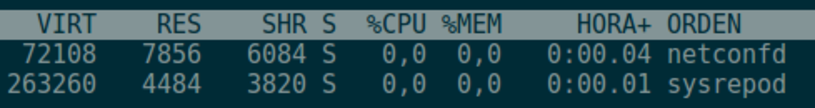
\includegraphics[scale=0.80]{Figures/consumoagentes.pdf}
		\caption{Demanda de recursos de las implementaciones analizadas.}
		\label{fig:consumoagentes}
	  \end{figure}
	\end{itemize}


	\subsubsection{Justificación de elección del agente}

	Presentado el análisis y las diferencias entre ambos proyectos, en esta sección se justificará la elección de Yuma123 como servidor que se instalará en el \textit{muxponder} de 40GB.
	\\
	
	Como se mencionó anteriormente, Sysrepo fue la primera implementación con la que se tuvo contacto y manipulación del protocolo \textit{NETCONF}. La razón por la que se optó empezar a familiarizarse con este, fue porque se encontró una gran cantidad de ejemplos y casos de uso a la hora de realizar los módulos \textit{YANG} y relacionarlos con la instrumentación y las aplicaciones Unix. Además, la instalación del proyecto en una computadora de escritorio fue sencilla (debido a la extensa documentación y las diferentes alternativas de instalación que brinda como ser \textit{dockers}, \textit{scripts} de instalación, etc).

	Sin embargo, no resultó de igual forma a la hora de realizar la compilación cruzada. La razón se debe a que Sysrepo tiene gran cantidad de dependencias como ser \textit{libyang, Google Protocol Buffers, protobuf-c, libev,} entre otros. Específicamente, se tuvo problemas para compilar la librería \textit{'protobuf-c'} para la arquitectura \textit{NIOS}, por lo que se abandonó el uso de esta herramienta. Además, como se vio anteriormente, la demanda de memoria principal y secundaria en Sysrepo excede a los recursos disponibles en el muxponder.
	\\

	En el caso de Yuma123 se logró compilar e instalar de manera correcta todas las librerías requeridas. Además, se realizaron scripts que facilitan dicha tarea para las siguientes arquitecturas: \textit{ARM, NIOS y \texttt{x86\_64}}. Cabe destacar que si bien los recursos que demanda Yuma123 son menores frente a Sysrepo, los mismos siguen siendo excesivos para el muxponder. Por lo tanto, se realizaron optimizaciones en la compilación del proyecto. Por ejemplo, se ha omitido la compilación de la librería \textit{SSH}, ya que el \textit{muxponder} ya la integra. Además, el proyecto incorpora una gran cantidad de módulos \textit{YANG} a modo de ejemplo, estos no son necesarios para el funcionamiento del mismo, por lo que también fueron omitidos. Por último, se destaca la herramienta yangdump brindada por Yuma123, la cual facilita de forma significativa el desarrollo de las librerías \textit{SIL} en \textit{C}.
	\\

	De esta forma, el factor determinante a la hora de elegir entre las distintas implementaciones \textit{NETCONF}, fue tener en cuenta las limitaciones técnicas del equipo, siendo Yuma123 el agente que mejor se adaptó a las mismas. 

 % Chapter Template

\chapter{Diseño e Implementación} % Main chapter title
% cSpell:words resizebox \textit{onosapi} usecase Mcast enrutamiento parencite includegraphics pcktprocactiv lstlisting iperf

\label{Chapter4} % Change X to a consecutive number; for referencing this chapter elsewhere, use 
% \ref{ChapterX} 
Para el desarrollo del proyecto será necesario implementar un sistema donde se puedan realizar pruebas y evaluar la correctitud del mismo. 

De esta forma, la primera sección de este capítulo comprende tanto el análisis del sistema como la topología utilizada. Específicamente, se estudiará su estructura, su comportamiento y sus requerimientos. 

En las secciones siguientes, se detallarán las aplicaciones desarrolladas que permiten cumplir con el objetivo del proyecto. En primer lugar, se hará un estudio del módulo \textit{YANG} implementado, el cual caracteriza y modela los datos del equipo. A continuación, se detallará el \textit{driver} implementado para lograr la comunicación entre el controlador y el dispositivo. Por último, se analizará la interfaz \textit{REST} y la \textit{GUI} desarrollada.

%----------------------------------------------------------------------------------------
%	SECTION 1
%----------------------------------------------------------------------------------------

\section{Entorno de trabajo}
En esta sección se detallan las características del sistema a implementar, descriptas en el lenguaje de especificación de sistemas SysML \parencite{sysml}. Se optó por este lenguaje de modelado ya que brinda una extensión a UML permitiendo combinar elementos del mundo físico (\textit{hardware}) con elementos del mundo lógico (\textit{software}). 

%-----------------------------------
%	SUBSECTION 1
%-----------------------------------

\subsection{Topología}

Se conformará una topología con el fin de poder identificar en una primera instancia, los requerimientos que debe cumplir el sistema. La misma, está basada en un caso de uso simple, en el cual se quiere brindar conectividad a dos clientes a través de un enlace óptico, este último conformado por dos \textit{muxponders}.  

Es importante identificar la presencia del controlador \textit{ONOS}, el cual gestionará la configuración de los equipos mediante el protocolo \textit{NETCONF}. En la figura \ref{fig:topologia} se muestra de forma general la topología planteada. 

Los dispositivos terminales A y B, se encuentran conectados al puerto cliente del \textit{muxponder} C y D, respectivamente. A su vez, el transmisor del \textit{muxponder} C se encuentra conectado al receptor del \textit{muxponder} D, y viceversa. Esto permite una comunicación bidireccional, donde ambos clientes pueden tener conectividad. 

Por otra parte, el controlador tiene una conexión con los \textit{muxponder} a través de los puertos de control de los mismos. 

\begin{figure}[H]
    \centering
    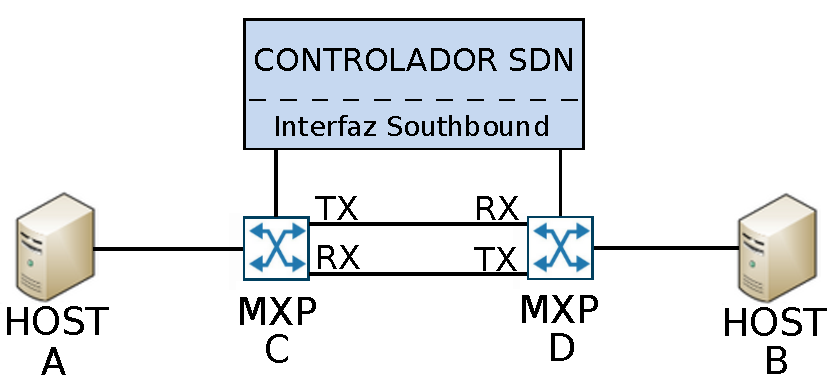
\includegraphics[scale=0.68]{Figures/topologia.pdf}
    \caption{Topología implementada en el proyecto.}
    \label{fig:topologia}
  \end{figure}


En la figura \ref{fig:topologiafis} se presenta cómo está dispuesta la conexión física de los equipos. En ella, se puede observar la alimentación de los equipos, los puertos clientes los cuales estarán conectados a los \textit{host} A y B antes mencionados. También, se observa las interfaces de línea conectadas entre sí, de tal manera que se permita una comunicación bidireccional entre los clientes. Por otro lado, las interfaces de control se conectan al controlador \textit{ONOS} tal cómo se mencionó anteriormente. 

\begin{comment}
A continuación, en la figura \ref{fig:topologiafis} se muestra como está dispuesta la conexión físicamente en los dispositivos. A la izquierda se tiene el \textit{muxponder} C, y a la derecha se encuentra el \textit{muxponder} D. Las interfaces de control de ambos dispositivos están conectadas al controlador \textit{ONOS}, mientras que los puertos clientes se encuentran conectados a los clientes A y B respectivamente. Por otra parte, las interfaces de línea se encuentran conectados entre los \textit{muxponder}, como se explicó anteriormente, con el fin de poder tener una comunicación bidireccional.
\end{comment}


\begin{figure}[H]
    \centering
    \resizebox{\textwidth}{!}{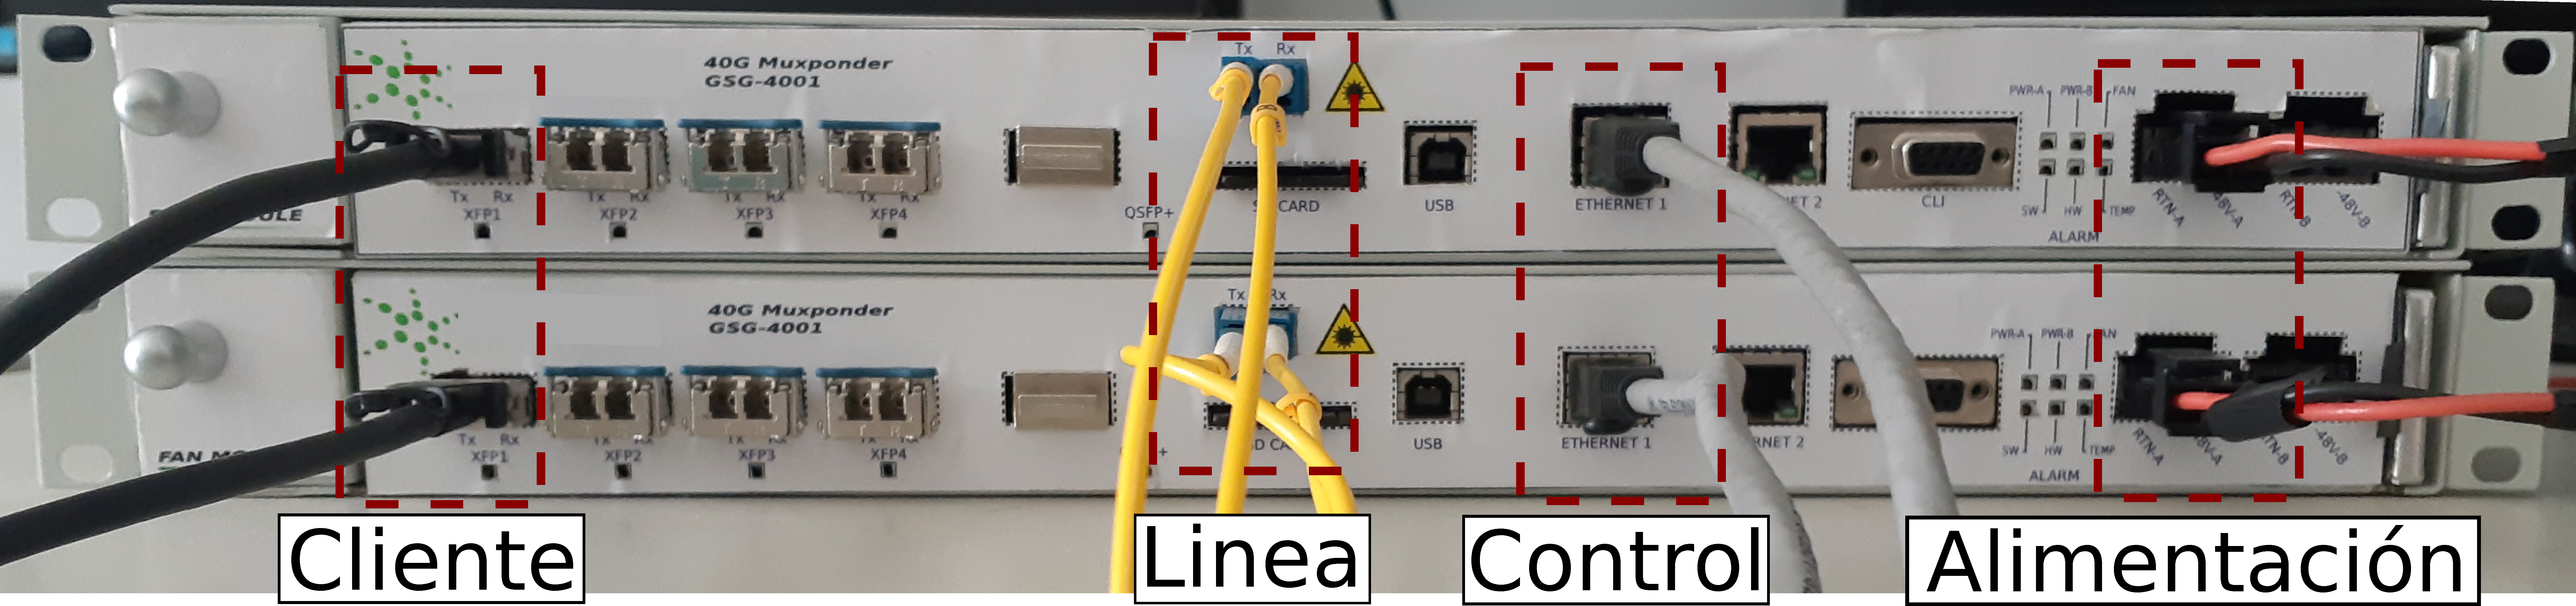
\includegraphics[scale=0.1]{Figures/mxpfisicos-min.pdf}}
    \caption{Conexión física de la topología.}
    \label{fig:topologiafis}
  \end{figure}


%-----------------------------------
%	SUBSECTION 2
%-----------------------------------
\subsection{Requerimientos del sistema}

Para establecer los requerimientos funcionales del sistema, se presentará en primer lugar un diagrama de caso de uso. Como se puede observar en la figura \ref{fig:caso_uso_admin}, el objeto principal del sistema es poder brindar al administrador un entorno donde pueda gestionar la configuración de los \textit{muxponders} mediante sus aplicaciones.

\begin{figure}[H]
    \centering
    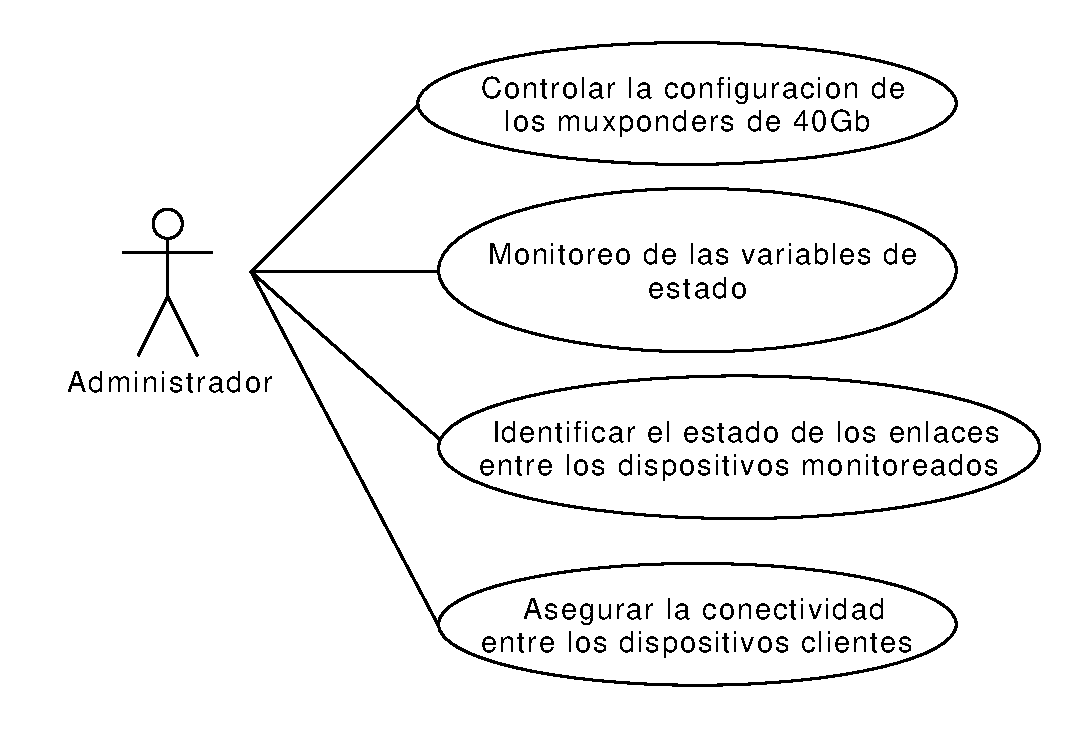
\includegraphics[scale=0.53]{Figures/caso_uso_admin.pdf}
    \caption{Caso de uso desde la perspectiva del administrador.}
    \label{fig:caso_uso_admin}
  \end{figure}

  En base a este diagrama, se pueden definir los requerimientos funcionales a nivel de sistema. La figura \ref{fig:req_sys} muestra una lista de los mismos. 
  
  Como requerimiento no funcional, se puede identificar la adición de nodos virtuales, los cuales no afectan a la funcionalidad del sistema pero brindan más flexibilidad y permiten conformar una topología más compleja.

  \begin{figure}[H]
    \centering
    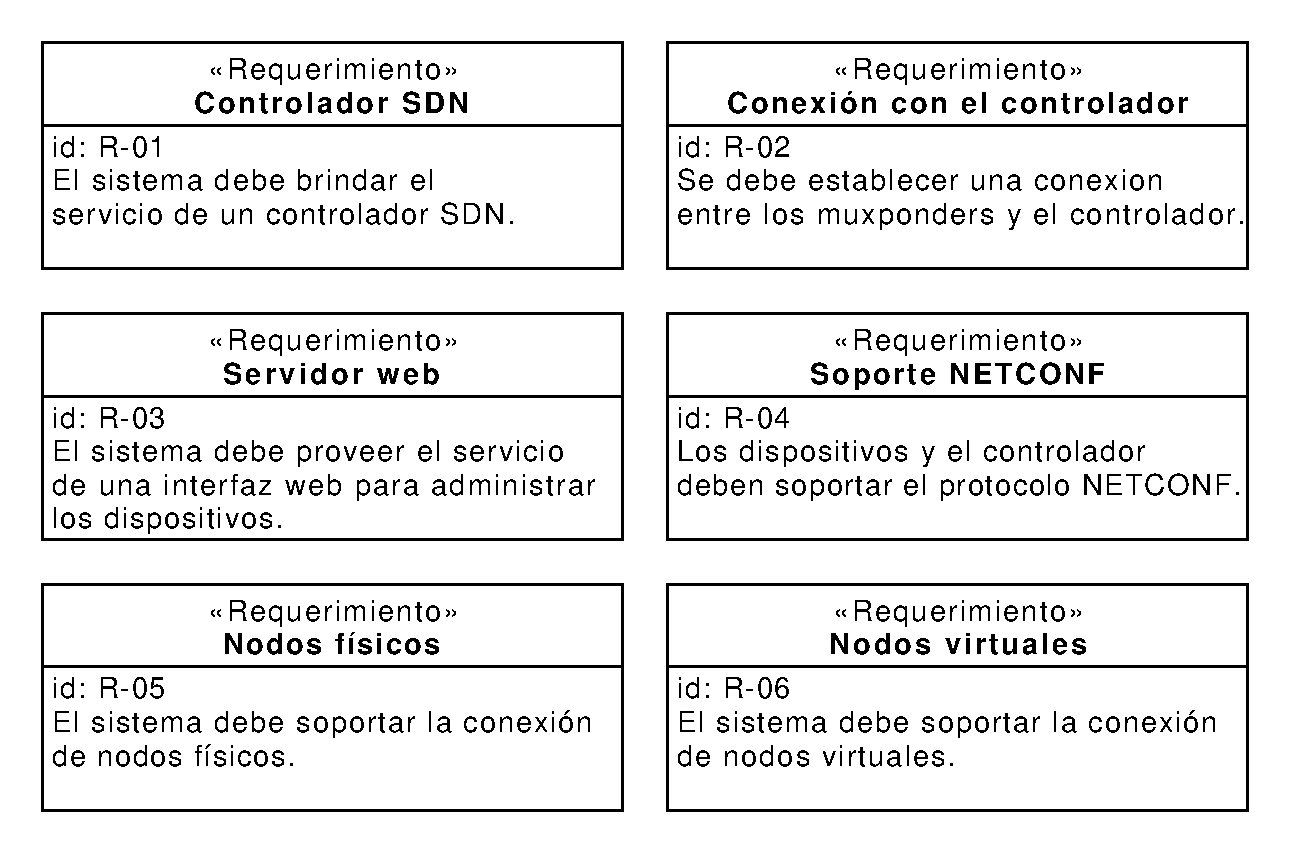
\includegraphics[scale=0.65]{Figures/req_sys.pdf}
    \caption{Requerimientos del sistema.}
    \label{fig:req_sys}
  \end{figure}


  Además, a partir del diagrama de caso de uso de la figura \ref{fig:caso_uso_admin}, se pueden identificar tres diagramas de actividades relacionadas. La figura \ref{fig:actividad_config}, muestra los flujos de actividad típicos que tendrá el sistema. 
  
  Para la actividad relacionada al monitoreo \ref{fig:actividad_config} (A), la aplicación \textit{WEB} realiza consultas periódicas al controlador con el fin de obtener información sobre los dispositivos. Así, se envía un mensaje HTTP con la operación GET desde la aplicación, el controlador procesa la petición y responde dicha consulta.

Por otra parte, para el flujo de actividad relacionado a las notificaciones que puede verse en la figura \ref{fig:actividad_config} (B), es el dispositivo quien emite inicialmente el mensaje mediante una notificación \textit{NETCONF}. En el controlador se procesa la notificación y se la registra como alarma.

Por último, se tiene el diagrama de actividad relacionado a la configuración del equipo \ref{fig:actividad_config} (C). El evento inicial para este caso, es la adición de una configuración desde la aplicación \textit{WEB}. Dicha configuración, una vez procesada se traduce en una solicitud POST HTTP que se envían hacia la \textit{Northbound interface} del controlador. Una vez recibida la solicitud, se realiza su procesamiento y se envía el mensaje de configuración \textit{NETCONF} a los dispositivos involucrados a través de la \textit{Southbound interface}.


  


  \begin{figure}[!h]
    \centering
    \begin{subfigure}[b]{0.43\textwidth}
        \centering
        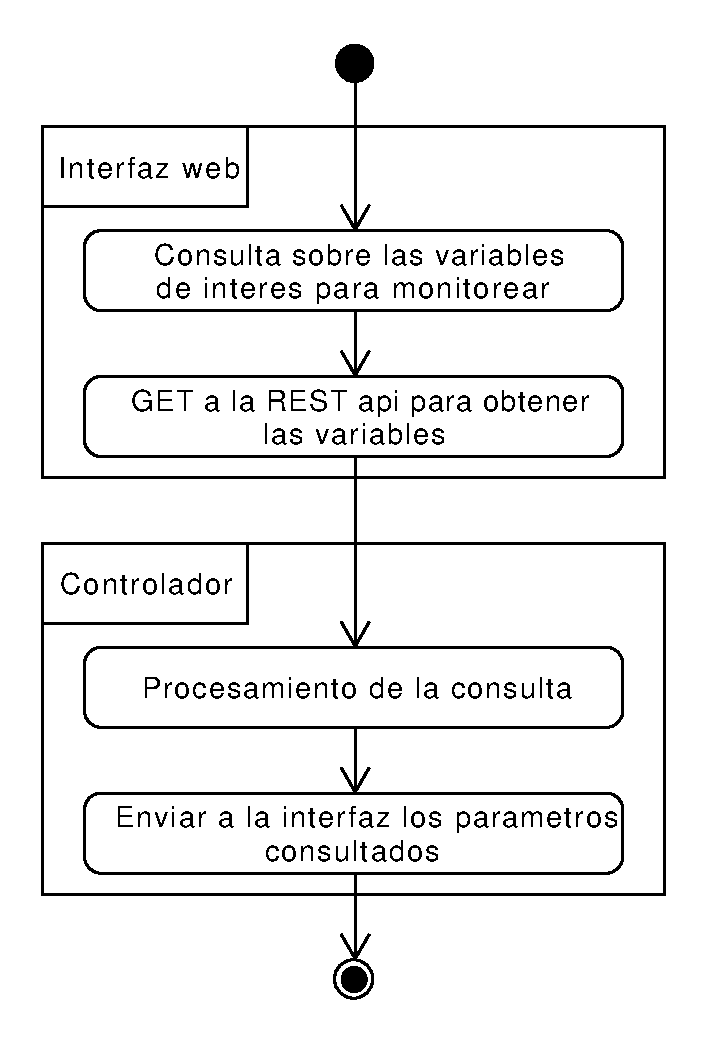
\includegraphics[width=\textwidth]{Figures/actividad_monitoreo.pdf}
        \caption{Actividad de monitoreo.}
    \end{subfigure}
    \quad
    \begin{subfigure}[b]{0.43\textwidth}  
        \centering 
        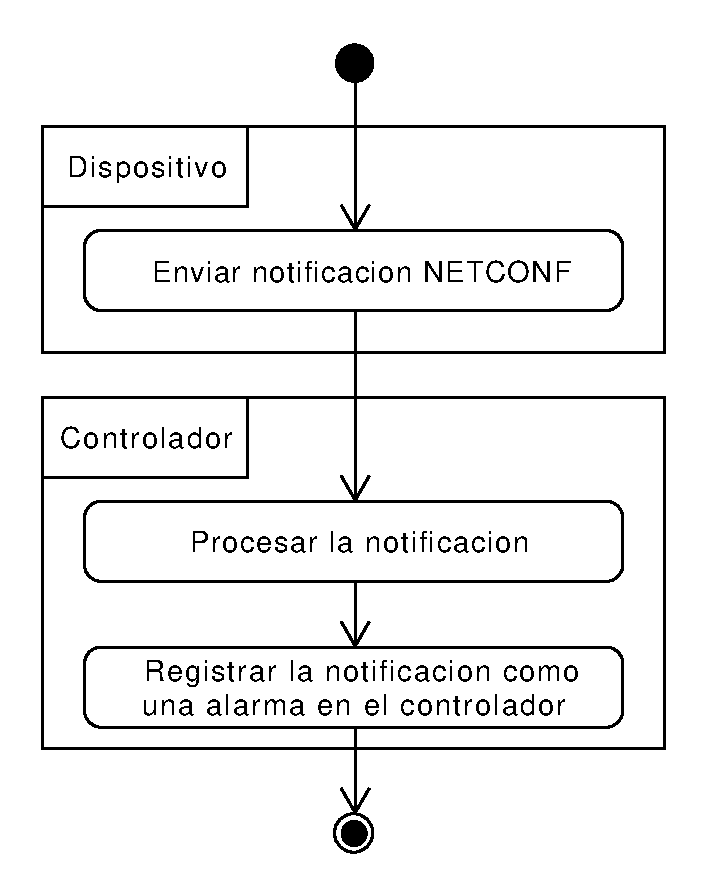
\includegraphics[width=\textwidth]{Figures/actividad_notif.pdf}
        \caption{Actividad de notificación.}
    \end{subfigure}
    \vskip\baselineskip
    \begin{subfigure}[b]{0.43\textwidth}   
        \centering 
        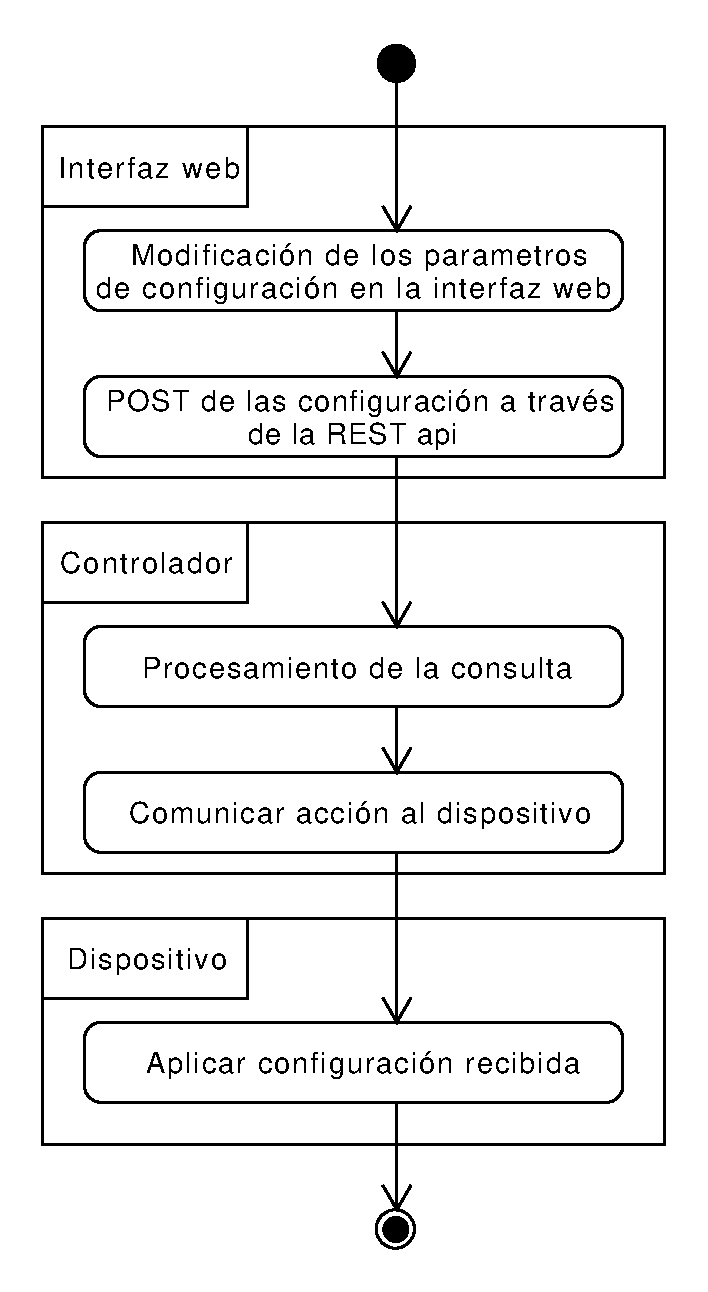
\includegraphics[width=\textwidth]{Figures/actividad_config_web.pdf}
        \caption{Actividad de configuración.}
    \end{subfigure}
    \caption{Diagramas de actividad del sistema.}
    \label{fig:actividad_config}
\end{figure}

\begin{comment}
  \begin{figure}[H]
    \centering
    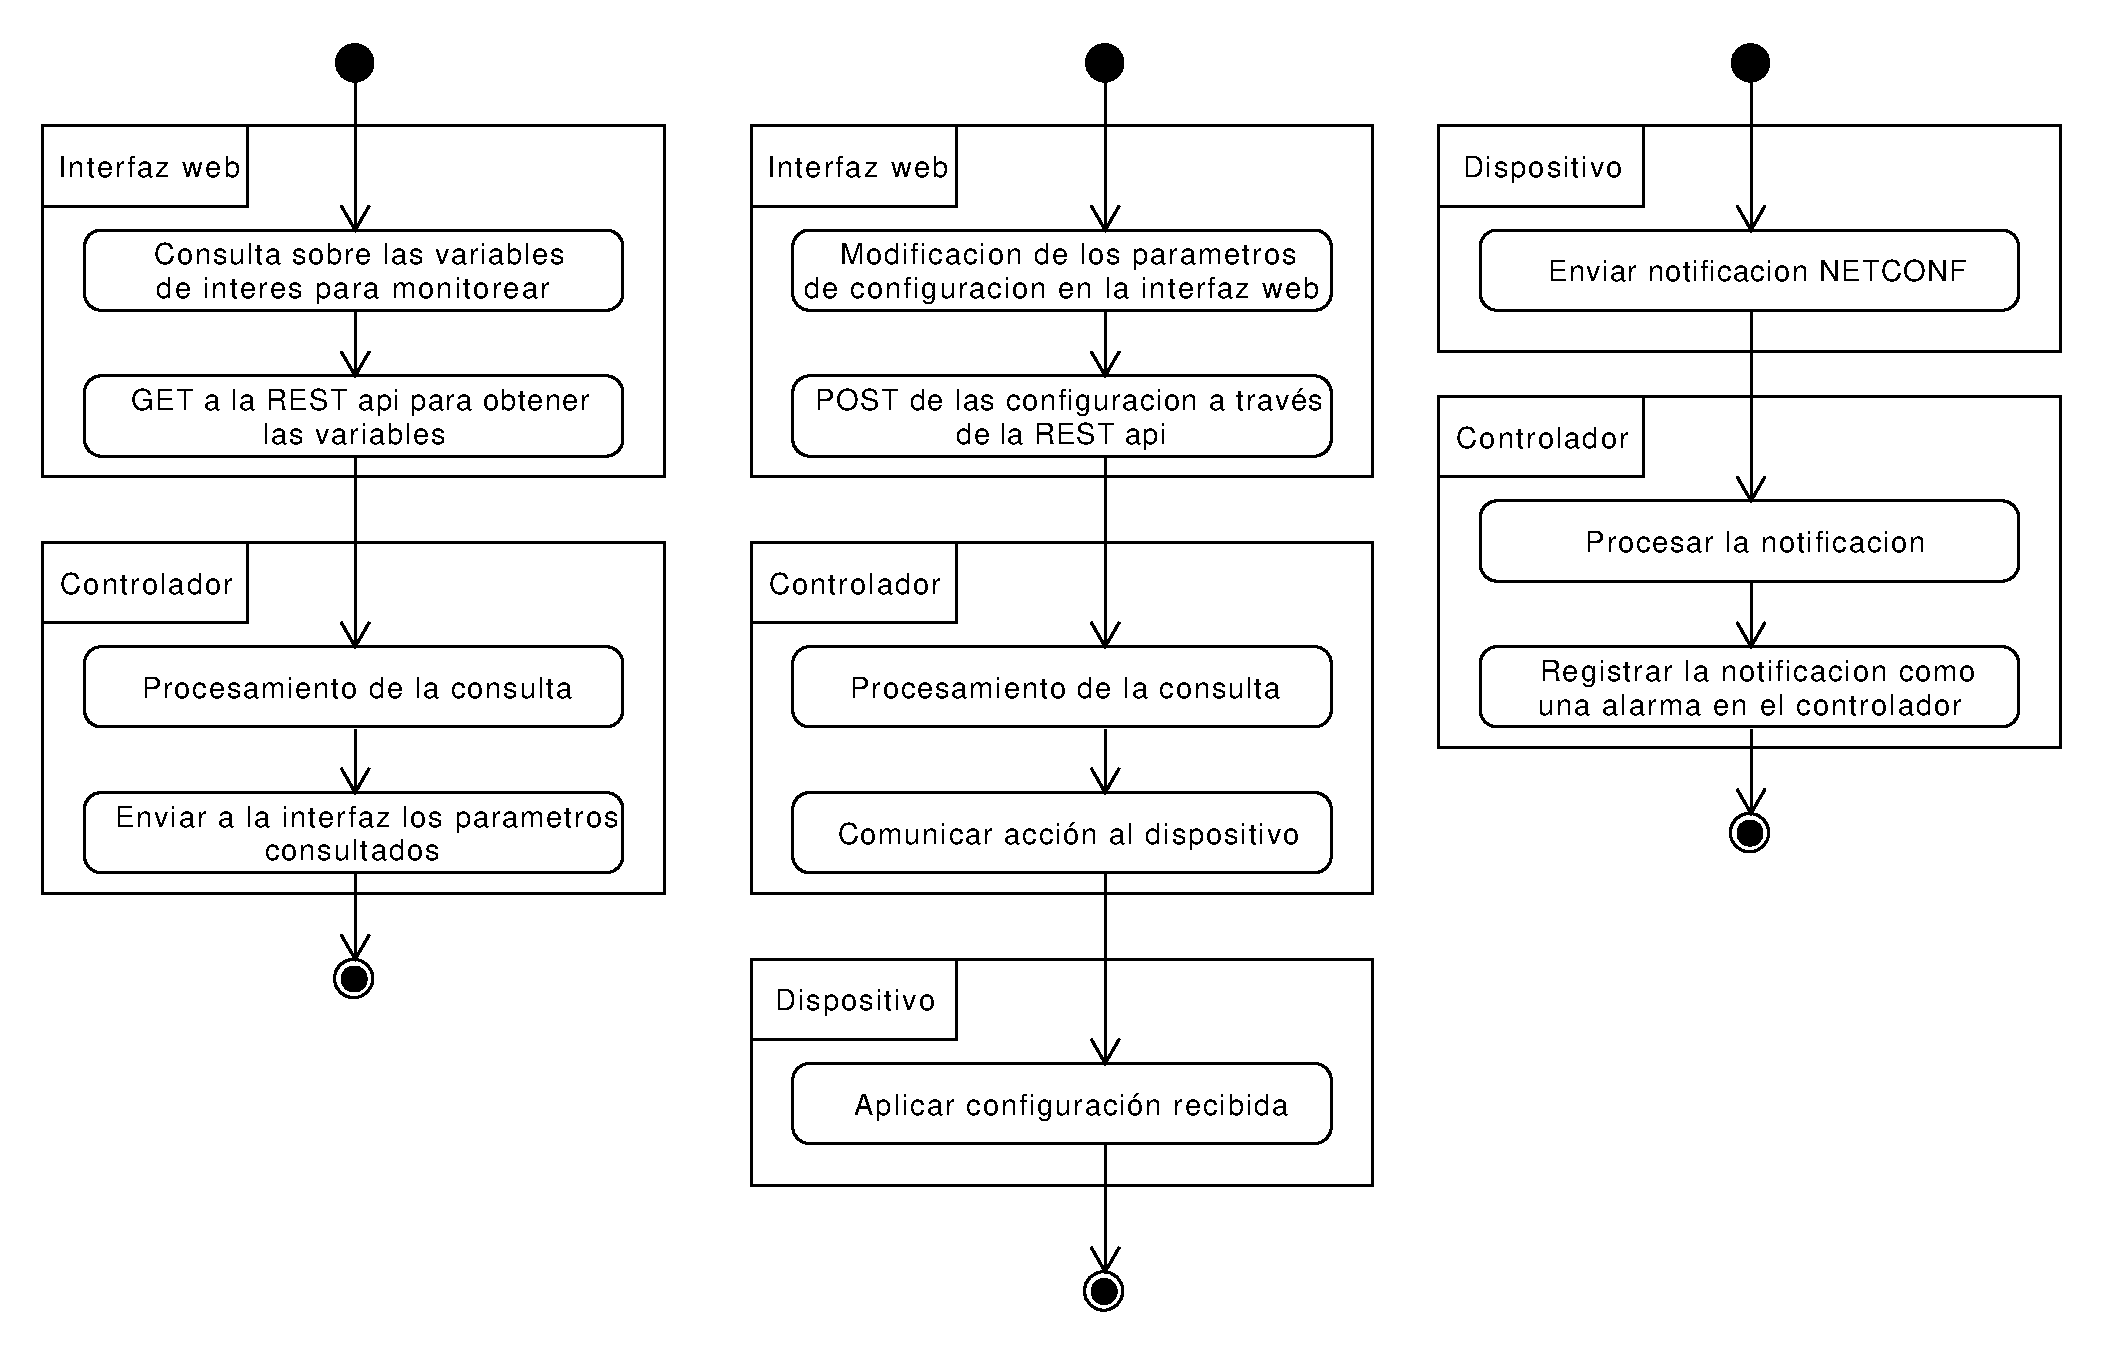
\includegraphics[scale=0.40]{Figures/actividad_config.pdf}
    \caption{Topología implementada en el proyecto.}
    \label{fig:actividad_config}
  \end{figure}
\end{comment}

\newpage
  %----------------------------------------------------------------------------------------
%	SECTION 2
%----------------------------------------------------------------------------------------

  \section{Integración del protocolo \textit{NETCONF} al \textit{muxponder}}
  La sección anterior deja claro que uno de los requerimientos de sistema será que tanto el controlador \textit{ONOS} como los dispositivos a monitorear soporten \textit{NETCONF} como protocolo de gestión de la configuración. 
  
  Como se vio en el capítulo anterior, el controlador soporta dicho protocolo, por lo que para cumplir con este requerimiento de sistema únicamente será necesario adaptar \textit{NETCONF} al dispositivo. 
  
  %-----------------------------------
%	SUBSECTION 1
%-----------------------------------

  \subsection{Requerimientos}

  Los requerimientos que deberá cumplir la integración del protocolo son los que se observan en la figura \ref{fig:req_netconf}.

  \begin{figure}[H]
    \centering
    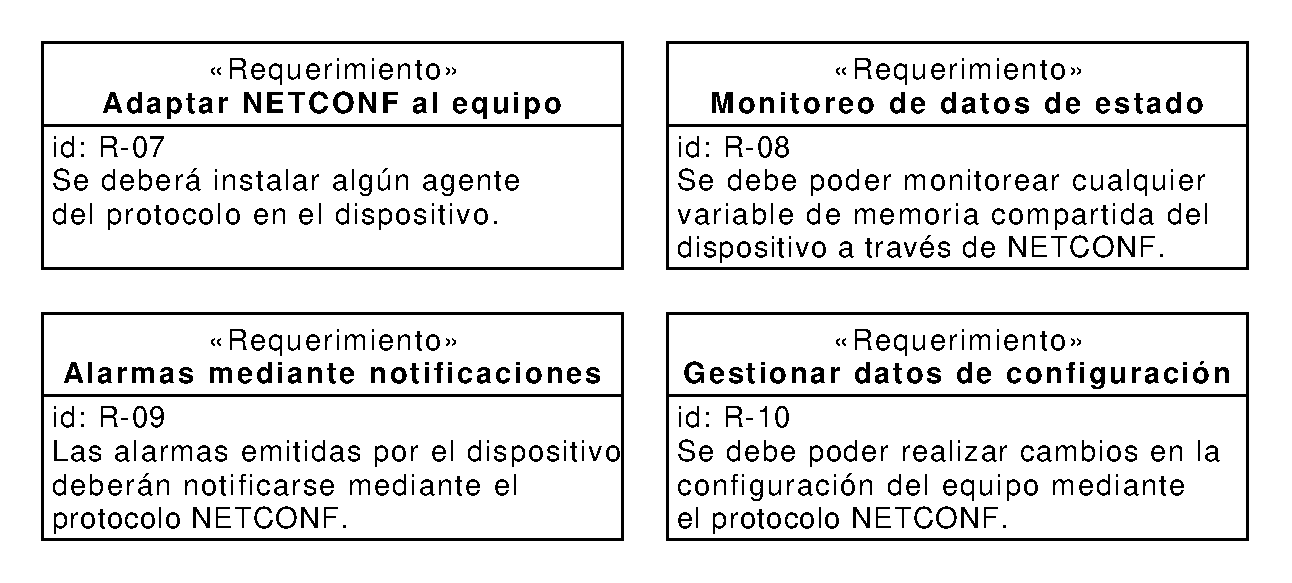
\includegraphics[scale=0.65]{Figures/req_netconf.pdf}
    \caption{Requerimientos para la integración del protocolo \textit{NETCONF}.}
    \label{fig:req_netconf}
  \end{figure}

%-----------------------------------
%	SUBSECTION 2
%-----------------------------------

  \subsection{Compilación e instalación del agente}
Siendo Yuma123 el agente que se eligió para integrar el protocolo en el equipo, en esta sección se detalla el procedimiento que se llevó a cabo para la compilación e instalación del agente en el \textit{muxponder}, con el fin de poder cumplir el requerimiento R-07.
\\

  En primer lugar, toda la tarea de compilación se realizó en una computadora de propósito general debido a los recursos limitados con los que cuenta el dispositivo. Para facilitar la compilación e instalación, se realizaron tres scripts los cuales se describen a continuación:

  \begin{itemize}
	\item \textbf{\texttt{Dockerfile}}: el objetivo de este \textit{script}, es el de realizar la compilación del proyecto Yuma123, dejando todas las librerías y los binarios en una carpeta que luego deberá copiarse en el dispositivo. Dockerfile \parencite{dockerfile}, es un archivo de texto que contiene los pasos e instrucciones que la herramienta Docker deberá seguir para construir una imagen. En el mismo, se indica una imagen de referencia (ubuntu:16.04) que servirá como base para la construcción. Luego, se descargan todas las librerías requeridas por el proyecto Yuma123 junto con los compiladores necesarios para realizar la compilación cruzada. A partir de aquí, se compila cada una de las librerías para la arquitectura objetivo (por ejemplo, NIOS II) y finalmente se compila también el proyecto Yuma123. Todos los binarios, librerías y cabeceras resultantes se encuentran en la carpeta '$/root/usrapp$' de la imagen Docker construida. Cabe destacar que se realizaron tres versiones del \textit{script}, de esta forma compilar para las arquitecturas NIOS II, ARM y \texttt{x86\_64}.
    
    \item \textbf{\texttt{remote\_install\_yuma.sh}}: \textit{script bash} que tiene la tarea de realizar la instalación del protocolo, compilado previamente con Docker y Dockerfile. Para ello, requiere de tres parámetros: usuario del dispositivo remoto, dirección IP del dispositivo remoto y la arquitectura deseada. Con estos parámetros, el \textit{script} realiza la instalación del agente mediante \textit{SSH} y \textit{SCP} \parencite{scpman}, copiando el contenido necesario de '$/root/usrapp$' que se generó con la construcción de la imagen Docker, al directorio '$/root/usrapp$' del dispositivo. Es importante mencionar que muchas de las librerías requeridas por Yuma123 son necesarias únicamente para la compilación y no para el funcionamiento del protocolo, por lo que este \textit{script} omitirá dichas librerías con el fin de reducir el tamaño que ocupa el agente en memoria.
    
    \item \textbf{\texttt{remote\_uninstall\_yuma.sh}}: requiere dos parámetros los cuales son el usuario del dispositivo remoto y la dirección IP del mismo. El objetivo de este \textit{script} es facilitar la desinstalación de todas las librerías relacionadas a Yuma123 del dispositivo.

\end{itemize}


\subsection{Diseño del módulo \textit{YANG}}

Para poder cumplir con los requerimientos R-08, R-09 y R-10 que se muestra en la figura \ref{fig:req_netconf}, se diseñó un módulo \textit{YANG} que contiene cinco secciones bien definidas, las cuales se describen a continuación: 

\begin{itemize}
	\item \textbf{Cabecera del módulo y declaraciones}: aquí se declara la estructura inicial del módulo \textit{YANG}. Se define un nombre y un prefijo, se realiza una descripción del mismo y por último se realiza la definición de los datos utilizados por el módulo. Cabe destacar que se definieron tres tipos de datos: ‘restricted-tipo-trafico‘, ‘restricted-tipo-fec-linea‘ y ‘restricted-tipo-fec-cliente‘. En ellos, se especifica a través de la directiva ‘enum’ cuales serán los valores aceptados que pueden tomar dichos tipos de datos. Por ejemplo, dado que la configuración del tipo de tráfico para este dispositivo únicamente admite dos valores (‘otu2‘ y ‘xge‘), es importante restringir el ingreso de algún otro valor ya que podría ocasionar errores en la configuración. Se puede observar una porción de esta sección en el código \ref{lstlisting:cabecera}, donde se detalla la cabecera del módulo y sus declaraciones.  

  \newpage
    \begin{lstlisting}[language=SHELXL, caption=Cabecera del módulo \textit{YANG}., label=lstlisting:cabecera]
        module cli-mxp {
            namespace 'http://fulgor.com/ns/cli-mxp';
            prefix 'cli-mxp';
            description
              'CLI para configurar el muxponder de 40G';
            revision '2018-06-24' {
                description
                  'Version 0.1.0';
            }

            typedef restricted-tipo-trafico {
                type enumeration {
                    enum 'otu2';
                    enum 'xge';
                  }
            }
              ...
              ...
              ...

    \end{lstlisting}

    \item \textbf{\textit{Container} \textit{YANG} de configuración}: en esta sección se declara un \textit{container} llamado ‘mux-config’. Aquí se describen todos los parámetros que admiten una configuración (por ejemplo, el tipo de fec de línea), a través de las declaraciones ‘leaf’. Un fragmento de esta sección puede observarse en el código \ref{lstlisting:config_container}, donde además se puede ver el uso de los tipos de datos definidos en la cabecera del módulo.
  
    \begin{lstlisting}[language=SHELXL, caption=\textit{Container} de configuración., label=lstlisting:config_container]
    container mux-config {
        description 'Parametros de la CLI';

        leaf tipo_trafico {
            description
              '[otu2|xge] especifica el tipo de tráfico.';
            type restricted-tipo-trafico;
        }
      
      ...
      ...
      ...
        
        list ports {
            key 'port';
            leaf port {
                type int16{
                    range '0 .. 6';
                }
                mandatory true;
            }

            leaf neighbor {
                mandatory true;
                type string;
            }
            
            leaf port_neighbor {
                mandatory true;
                type string;
            }
        }
    }
    \end{lstlisting}

    \item \textbf{\textit{Container} \textit{YANG} de estado}: de igual forma, se realizaron \textit{containers} para los datos de estado los cuales no admiten una escritura de valores y son necesarios para monitorear el dispositivo. El código \ref{lstlisting:state_container} presenta una parte de esta sección del módulo, donde puede apreciarse la directiva ’config false’, la cual indica que el \textit{container} no admitirá datos de configuración.  

    \begin{lstlisting}[language=SHELXL, caption=\textit{Container} de estado., label=lstlisting:state_container]
    container mux-state {
        description 'Representa a datos de estado del dispositivo.';
        
        config false;

        leaf fpga_temperature_state {
            description 'Temperatura de la FPGA';
            type decimal64 {
                fraction-digits 2;
            }
        }
   
        leaf device_boardId {
            description 'Identificador unico del dispositivo';
            type string;
        }
        ...
        ...
        ...
    \end{lstlisting}


    \item \textbf{Definición de \textit{RPC}}: como se estudió en capítulos anteriores, \textit{NETCONF} permite definir \textit{RPC} propias de un módulo con el fin de extender la funcionalidad de los dispositivos. Se define así una \textit{RPC} cuya utilidad será la de poder indicar al agente cuándo debe aplicar la configuración que contiene el \textit{container} 'mux-config' en el dispositivo. El código \ref{lstlisting:RPC} muestra dicha sección del módulo. En ella, se puede notar que la \textit{RPC} admite una respuesta de la operación solicitada, la cual está contenida en la \textit{leaf} 'respuesta-mux-apply-config' y es de tipo \textit{String}. En este mensaje se indica el resultado de la operación.

    

    \begin{lstlisting}[language=SHELXL, caption=Declaración de \textit{RPC}., label=lstlisting:RPC]
    rpc mux-apply-config {        
        description 'RPC que aplica los cambios de configuracion';
        output {
            leaf respuesta-mux-apply-config {
                type string;
            }
        }
    }
    \end{lstlisting}

    \item \textbf{Definición de notificación}: por último, el módulo tiene una sección donde se declara una notificación. Dicho mensaje será utilizado para indicar a las sesiones conectadas y suscritas las diferentes alarmas que produzca el dispositivo. Estos mensajes se transportan mediante notificaciones del protocolo \textit{NETCONF}. El propósito de estos mensajes es el de, por ejemplo, reportar mediante una alarma si un enlace con un dispositivo vecino se cayó, si el dispositivo supera la temperatura umbral, etc. Se puede observar en el código \ref{lstlisting:notif} la declaración de la notificación en el módulo. El mensaje estará contenido dentro de la \textit{leaf} ’INFO’, en la cual se especifica de forma obligatoria con la directiva ’mandatory’ cuál será el mensaje que se enviará como notificación.

    \begin{lstlisting}[language=SHELXL, caption=Declaración de notificación., label=lstlisting:notif]
    notification mux-notify {
        leaf INFO {
            type string;
            mandatory 'true';
        }
    }
    \end{lstlisting}

\end{itemize}

\subsection{Diseño de la librería \textit{C} para el agente \textit{NETCONF}}


  Teniendo en cuenta las aplicaciones integradas en el \textit{muxponder} las cuales fueron explicadas en el capítulo anterior, se procede a detallar el diseño de la librería en el lenguaje \textit{C}. Para ello, se utilizó la herramienta \textit{yangdump} del proyecto Yuma123, la cual genera un esqueleto de la aplicación a partir de un módulo \textit{YANG} dado. Se forman así dos archivos, uno con extensión '.h' (\textit{headers}) y otro con extensión '.c' (código fuente). 
  

  En el primero, la herramienta declara todas las variables, funciones y los tipos de datos que va a utilizar la librería. 

  Por otra parte, el segundo archivo contiene la estructura de la aplicación en sí. En el, se encuentran implementadas todas las funciones declaradas en el archivo con extensión '.h', las cuales llamará el agente en caso de que ingrese un mensaje referido al módulo \textit{YANG} en cuestión. Todo el desarrollo de la aplicación y la relación entre la instrumentación del dispositivo con el módulo \textit{YANG} se encuentra en este archivo. 


  Con el fin de explicar cómo se desarrolló esta aplicación, se distinguen dos flujos de actividades bien definidos, uno para las operaciones que son sincrónicas con los mensajes que envía el cliente, y otro para aquellas que sean asíncronas a los mensajes del mismo. 

  Para el primer grupo, se tiene entonces las operaciones como obtención de un dato de estado o de configuración, modificación de un dato de configuración y ejecución de \textit{RPC}, mientras que el segundo grupo contempla el envío de notificaciones, las cuales son asíncronas a las operaciones del cliente.
  

  Se muestra el comportamiento de este primer grupo en el diagrama de actividad de la figura \ref{fig:actividad_modulo_sinc}. Cada vez que llega un mensaje \textit{NETCONF} al agente Yuma123, el mismo procesa y verifica a qué módulo \textit{YANG} hace referencia el mensaje y qué tipo de operación requiere el cliente. 

  Si la operación es una consulta por una variable de estado o de configuración, el agente realiza una llamada a una función relacionada a la variable consultada. En dicha función, lo que se hace es tomar el valor de memoria compartida del dispositivo, castear el mismo según indique el modulo \textit{YANG} (\textit{string, int, uint,} etc) y por último, emitir una respuesta al cliente con el valor del dato consultado.

  Por otra parte, si la operación es la de editar una variable de configuración, el agente llama a una función de la librería \textit{C} relacionada al módulo en cuestión, donde se actualiza el valor de dicha variable. Además, el agente emite un mensaje con el resultado de la operación. 

  Por último, si la operación trata de una \textit{RPC} definida en el módulo \textit{YANG}, el agente llama a la función relacionada a la \textit{RPC} la cual contiene las instrucciones para efectuar la tarea solicitada. En este caso, se tiene una \textit{RPC} que indica cuándo se deberá aplicar la configuración en el dispositivo. Así, al momento de llamar a esta \textit{RPC} el agente copia los valores de los datos de configuración necesarios (tipo de tráfico, tipo fec de cliente, tipo fec línea, etc) y los aplica haciendo uso del binario 'muxponder'.

  \begin{figure}[H]
    \centering
    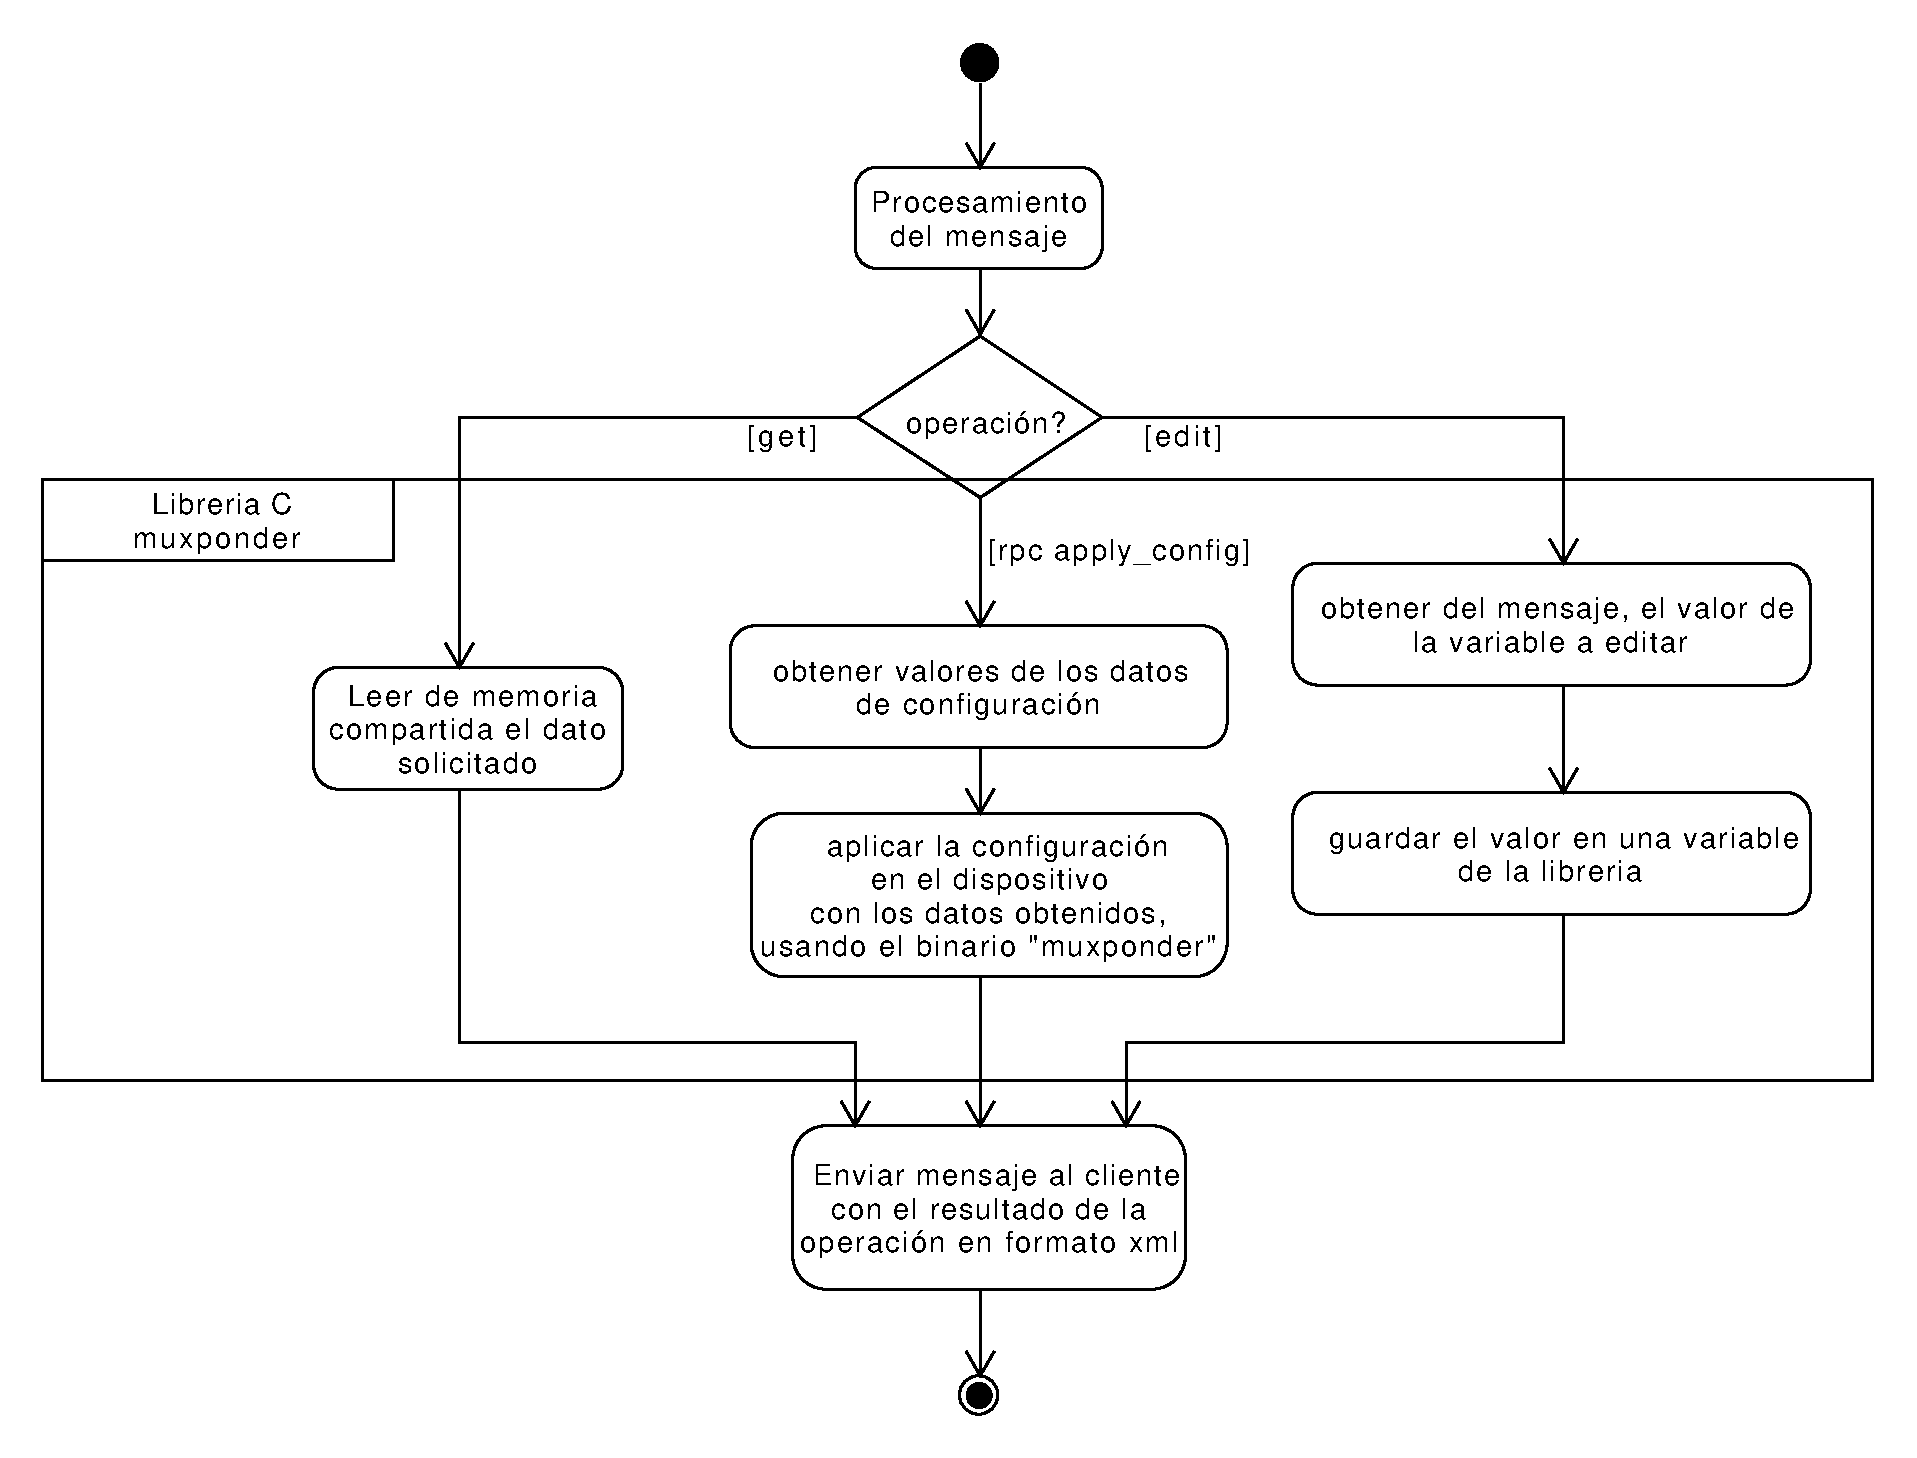
\includegraphics[scale=0.45]{Figures/actividad_modulo_sinc.pdf}
    \caption{Diagrama de actividad de las operaciones síncronas con el cliente.}
    \label{fig:actividad_modulo_sinc}
  \end{figure}

  Por otra parte, el grupo relacionado a las operaciones asíncronas con los mensajes del cliente, no es otra cosa que la operación de envío de notificaciones mediante el protocolo \textit{NETCONF}. Para ello, la librería desarrollada en \textit{C} crea un hilo que examina periódicamente cada tres segundos la memoria compartida del dispositivo. 
  
  La razón por la cual se examina cada tres segundos está relacionada con la aplicación 'monitor', la cual actualiza los valores de memoria compartida con esa frecuencia.

  Al examinar los valores de las alarmas, las compara con la información antigua que se tenía almacenada sobre las mismas. Si la información es igual, no se envían notificaciones a las sesiones. En cambio, si la información actual es diferente a la información anterior, será necesario notificar a las sesiones suscritas este nuevo estado de las alarmas. Así, tanto el nombre de la alarma como su nuevo estado son enviados a través de la notificación definida en el código \ref{lstlisting:notif}, haciendo uso de la \textit{leaf} INFO.
  
  Un diagrama de actividad de estas operaciones se puede observar en la figura \ref{fig:actividad_modulo_notif}.

  \begin{figure}[H]
    \centering
    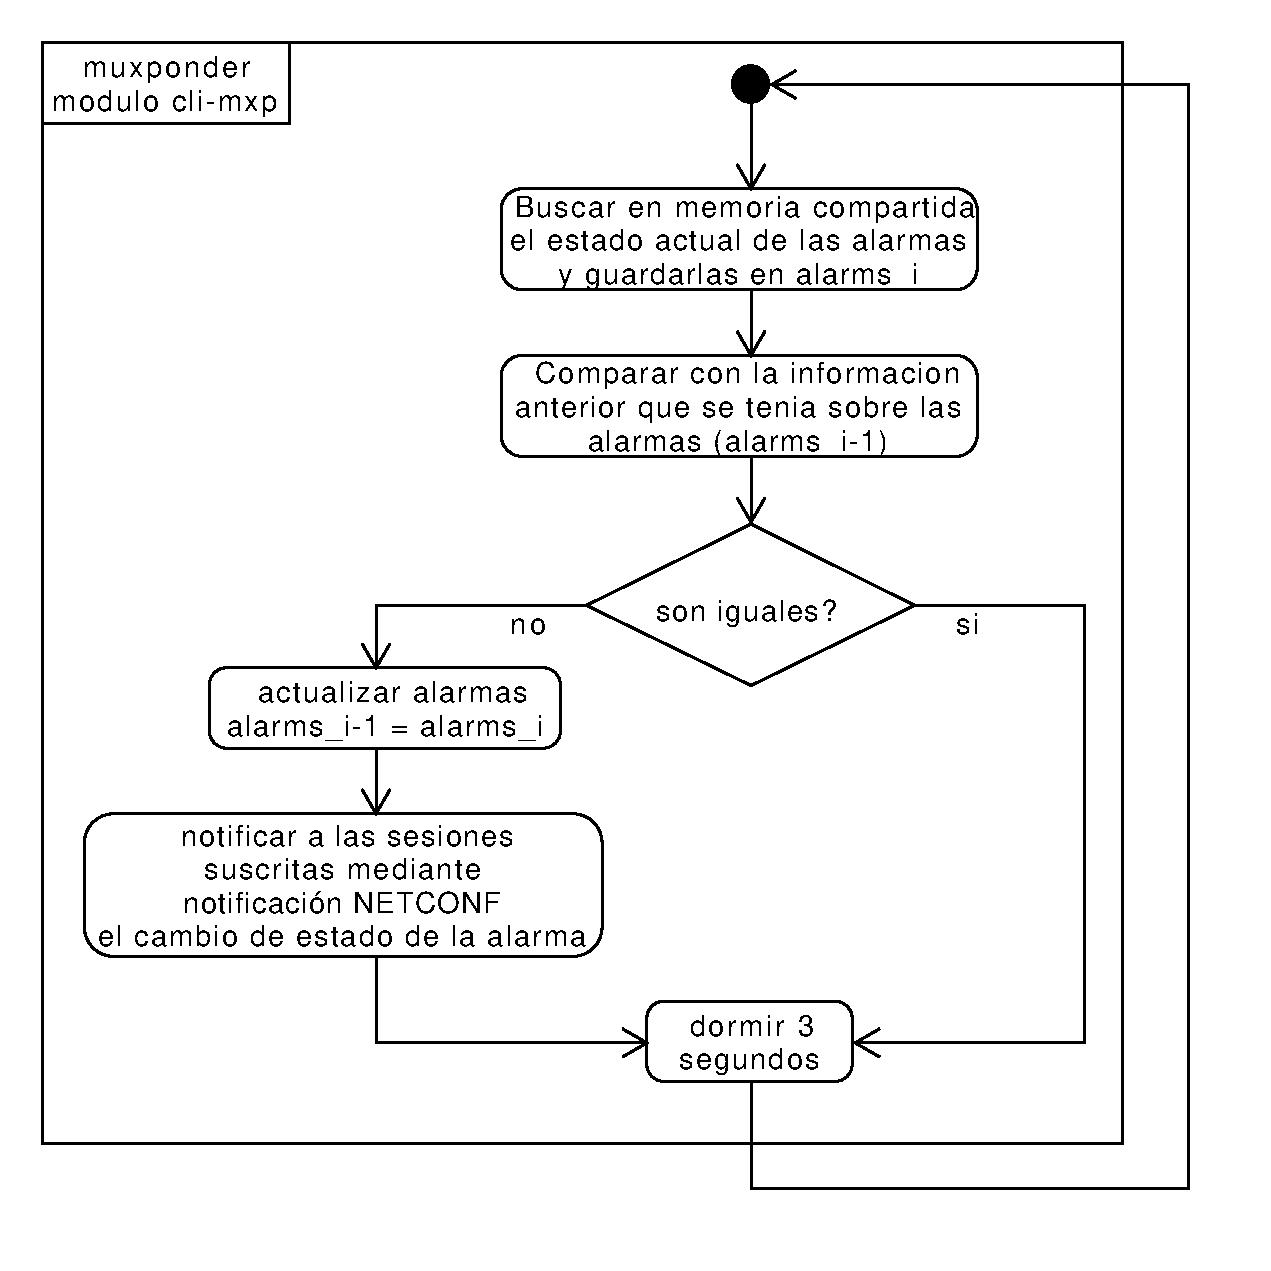
\includegraphics[scale=0.50]{Figures/actividad_modulo_notif.pdf}
    \caption{Diagrama de actividad de las notificaciones.}
    \label{fig:actividad_modulo_notif}
  \end{figure}


  \section{Diseño del \textit{driver}} 
  Como se vio en capítulos anteriores, \textit{ONOS} se comunica con los dispositivos a través de tres componentes de la interfaz \textit{Southbound}: \textit{Providers}, \textit{Protocols} y \textit{Drivers}.
  
  Así, para poder indicar al controlador cuáles serán las operaciones y los comportamientos específicos del \textit{muxponder} de 40GB, será necesario desarrollar un \textit{driver} (Java) en la interfaz \textit{Southbound} del controlador. 

  \subsection{Requerimientos}
  A fin de cubrir las necesidades del administrador, visto en el caso de uso de la figura \ref{fig:caso_uso_admin}, el \textit{driver} desarrollado deberá cumplir con los requerimientos funcionales de la figura \ref{fig:req_driver}.
  
  \begin{figure}[H]
    \centering
    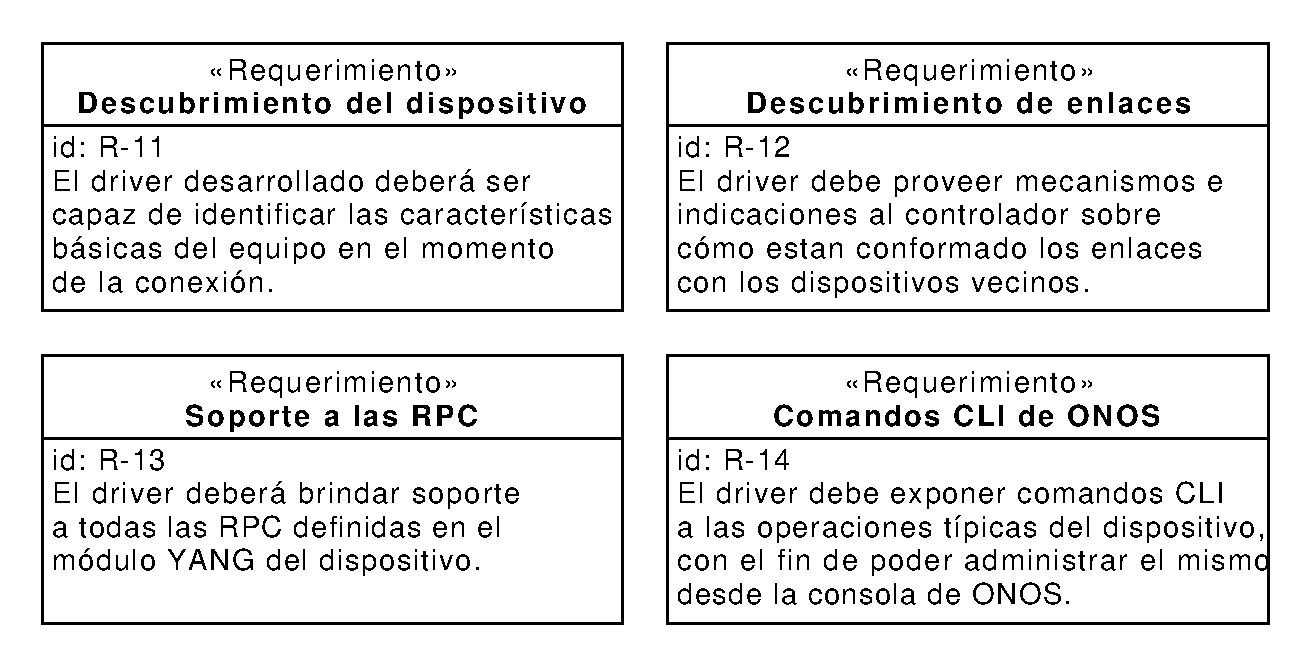
\includegraphics[scale=0.65]{Figures/req_driver.pdf}
    \caption{Requerimientos para el \textit{driver} de la interfaz \textit{Southbound}.}
    \label{fig:req_driver}
  \end{figure}

  \subsection{Descubrimiento del dispositivo} \label{driverr}
  El controlador \textit{ONOS} reconoce la presencia de un nuevo dispositivo a través de un mensaje en formato JSON, el cual contiene información como la dirección IP del equipo, el \textit{driver} que describe sus comportamientos, el protocolo que utiliza, entre otra información de utilidad. 
  
  Un ejemplo de este mensaje se muestra en el código \ref{lstlisting:JSON}. Dicho mensaje, es enviado al controlador haciendo uso del comando de \textit{ONOS} 'onos-netcfg' \parencite{onosconfserv}.

  \begin{lstlisting}[language=SHELXL, caption=Mensaje JSON con información del dispositivo., label=lstlisting:JSON]
    {
        'devices': {
            'netconf:172.16.0.141:830': {
            'netconf': {
                'ip': '172.16.0.141',
                'port': 830,
                'username': 'user',
                'password': 'pass',
            },
            'basic': {
                'driver': 'altura-netconf'
           }
        }
    }
    \end{lstlisting}


    Al momento de indicar al controlador \textit{ONOS} la presencia de un nuevo dispositivo, el mismo hace una llamada por única vez a la función \textit{DeviceDescriptionDiscovery}, la cual se encuentra implementada en el \textit{driver} indicado por el archivo JSON. 

    Esta función, tiene la tarea de descubrir las características más generales del equipo, como ser la versión de \textit{software} y de \textit{hardware} del mismo, el número de puertos disponibles, el identificador único del dispositivo, etc.

    Con más detalle, la función inicia la sesión \textit{SSH} del protocolo \textit{NETCONF}, espera a que termine el intercambio de capacidades entre cliente y servidor y por último envía un mensaje \textit{NETCONF} al servidor solicitando con la operación 'GET' los siguientes datos de estado:  
    
    \begin{itemize}
        \item información del fabricante.
        \item versión de \textit{hardware}.
        \item versión de \textit{software}.
        \item identificador único del equipo.
        \item alarmas activas en el equipo.
    \end{itemize}


    La figura \ref{fig:actividad_driver_descr} muestra el flujo de actividad típico que tendría el controlador \textit{ONOS} al momento de agregarse un nuevo dispositivo administrado por el \textit{driver} desarrollado.
    
    \begin{figure}[H]
        \centering
        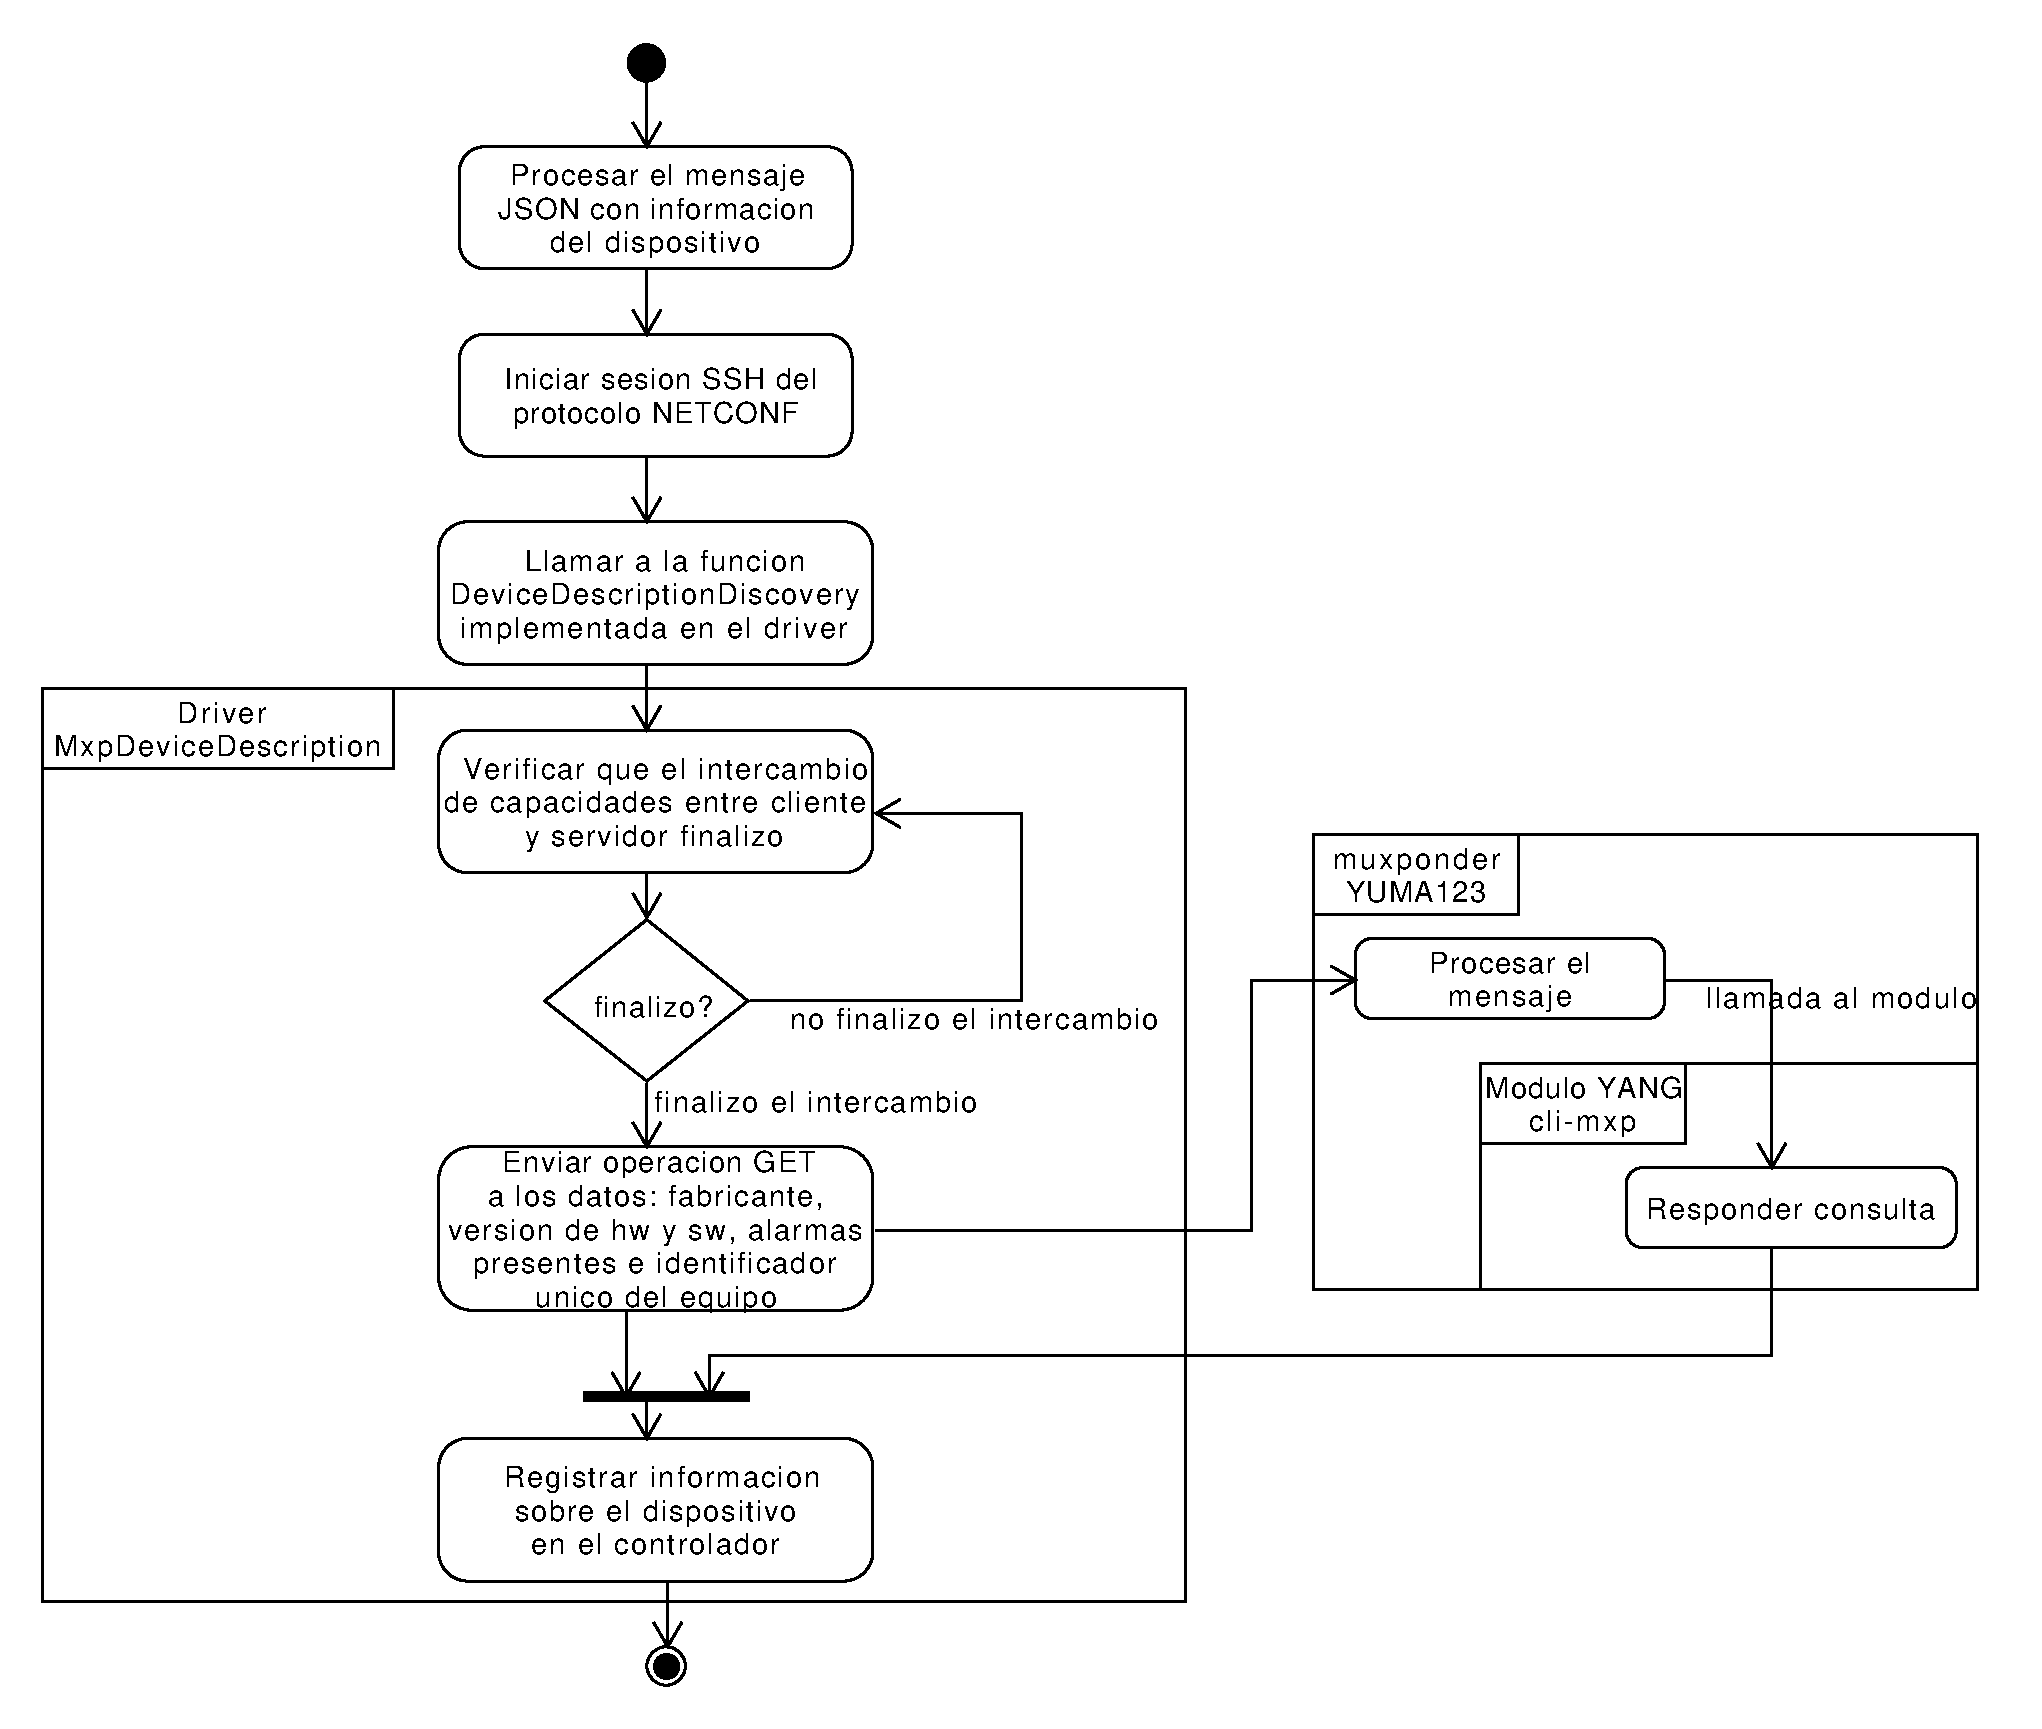
\includegraphics[scale=0.45]{Figures/actividad_driver_descr.pdf}
        \caption{Diagrama de actividad de la función \textit{DeviceDescriptionDiscovery}.}
        \label{fig:actividad_driver_descr}
      \end{figure}

\subsection{Descubrimiento de Enlaces} \label{driverlink}

El \textit{driver} también debe proveer un mecanismo para indicar al controlador cómo se componen los enlaces entre los diferentes dispositivos administrados. Para ello, el controlador \textit{ONOS} brinda una interfaz llamada \textit{LinkDiscovery}, la cual se deberá implementar en el \textit{driver}. 

Así, el controlador llama periódicamente a esta función (cada 30 segundos de forma predeterminada, pudiéndose cambiar este tiempo desde la \textit{CLI}) para corroborar el estado de los enlaces. 

Con más detalle, lo que realiza esta función es enviar periódicamente a los dispositivos un mensaje \textit{NETCONF} con la operación GET-CONFIG, consultando por los datos 'port', 'neighbor' y 'port-neighbor' del \textit{container} 'mux-config', estos datos pueden verse representados en el módulo \textit{YANG}, en el código \ref{lstlisting:config_container}. A continuación, se explica de forma breve la función de cada uno de estos datos:

\begin{itemize}
	\item \textbf{port}: indica el puerto del dispositivo local al cual se conectará un vecino.
    
    \item \textbf{neighbor}: contiene el identificador único del dispositivo vecino.
    
    \item \textbf{port-neighbor}: indica el puerto del dispositivo vecino que se conectará en 'port' y con el que deberá formar el enlace.
\end{itemize}

Con esta información, el \textit{driver} informa al controlador que forme un enlace óptico entre ambos dispositivos. Si alguno de los dispositivos involucrados contiene alarmas registradas respecto al enlace de línea del \textit{muxponder}, concretamente alarmas relativas al receptor, el enlace no se forma. El diagrama de actividad de la figura \ref{fig:actividad_link} muestra lo explicado anteriormente.

\begin{figure}[!h]
    \centering
    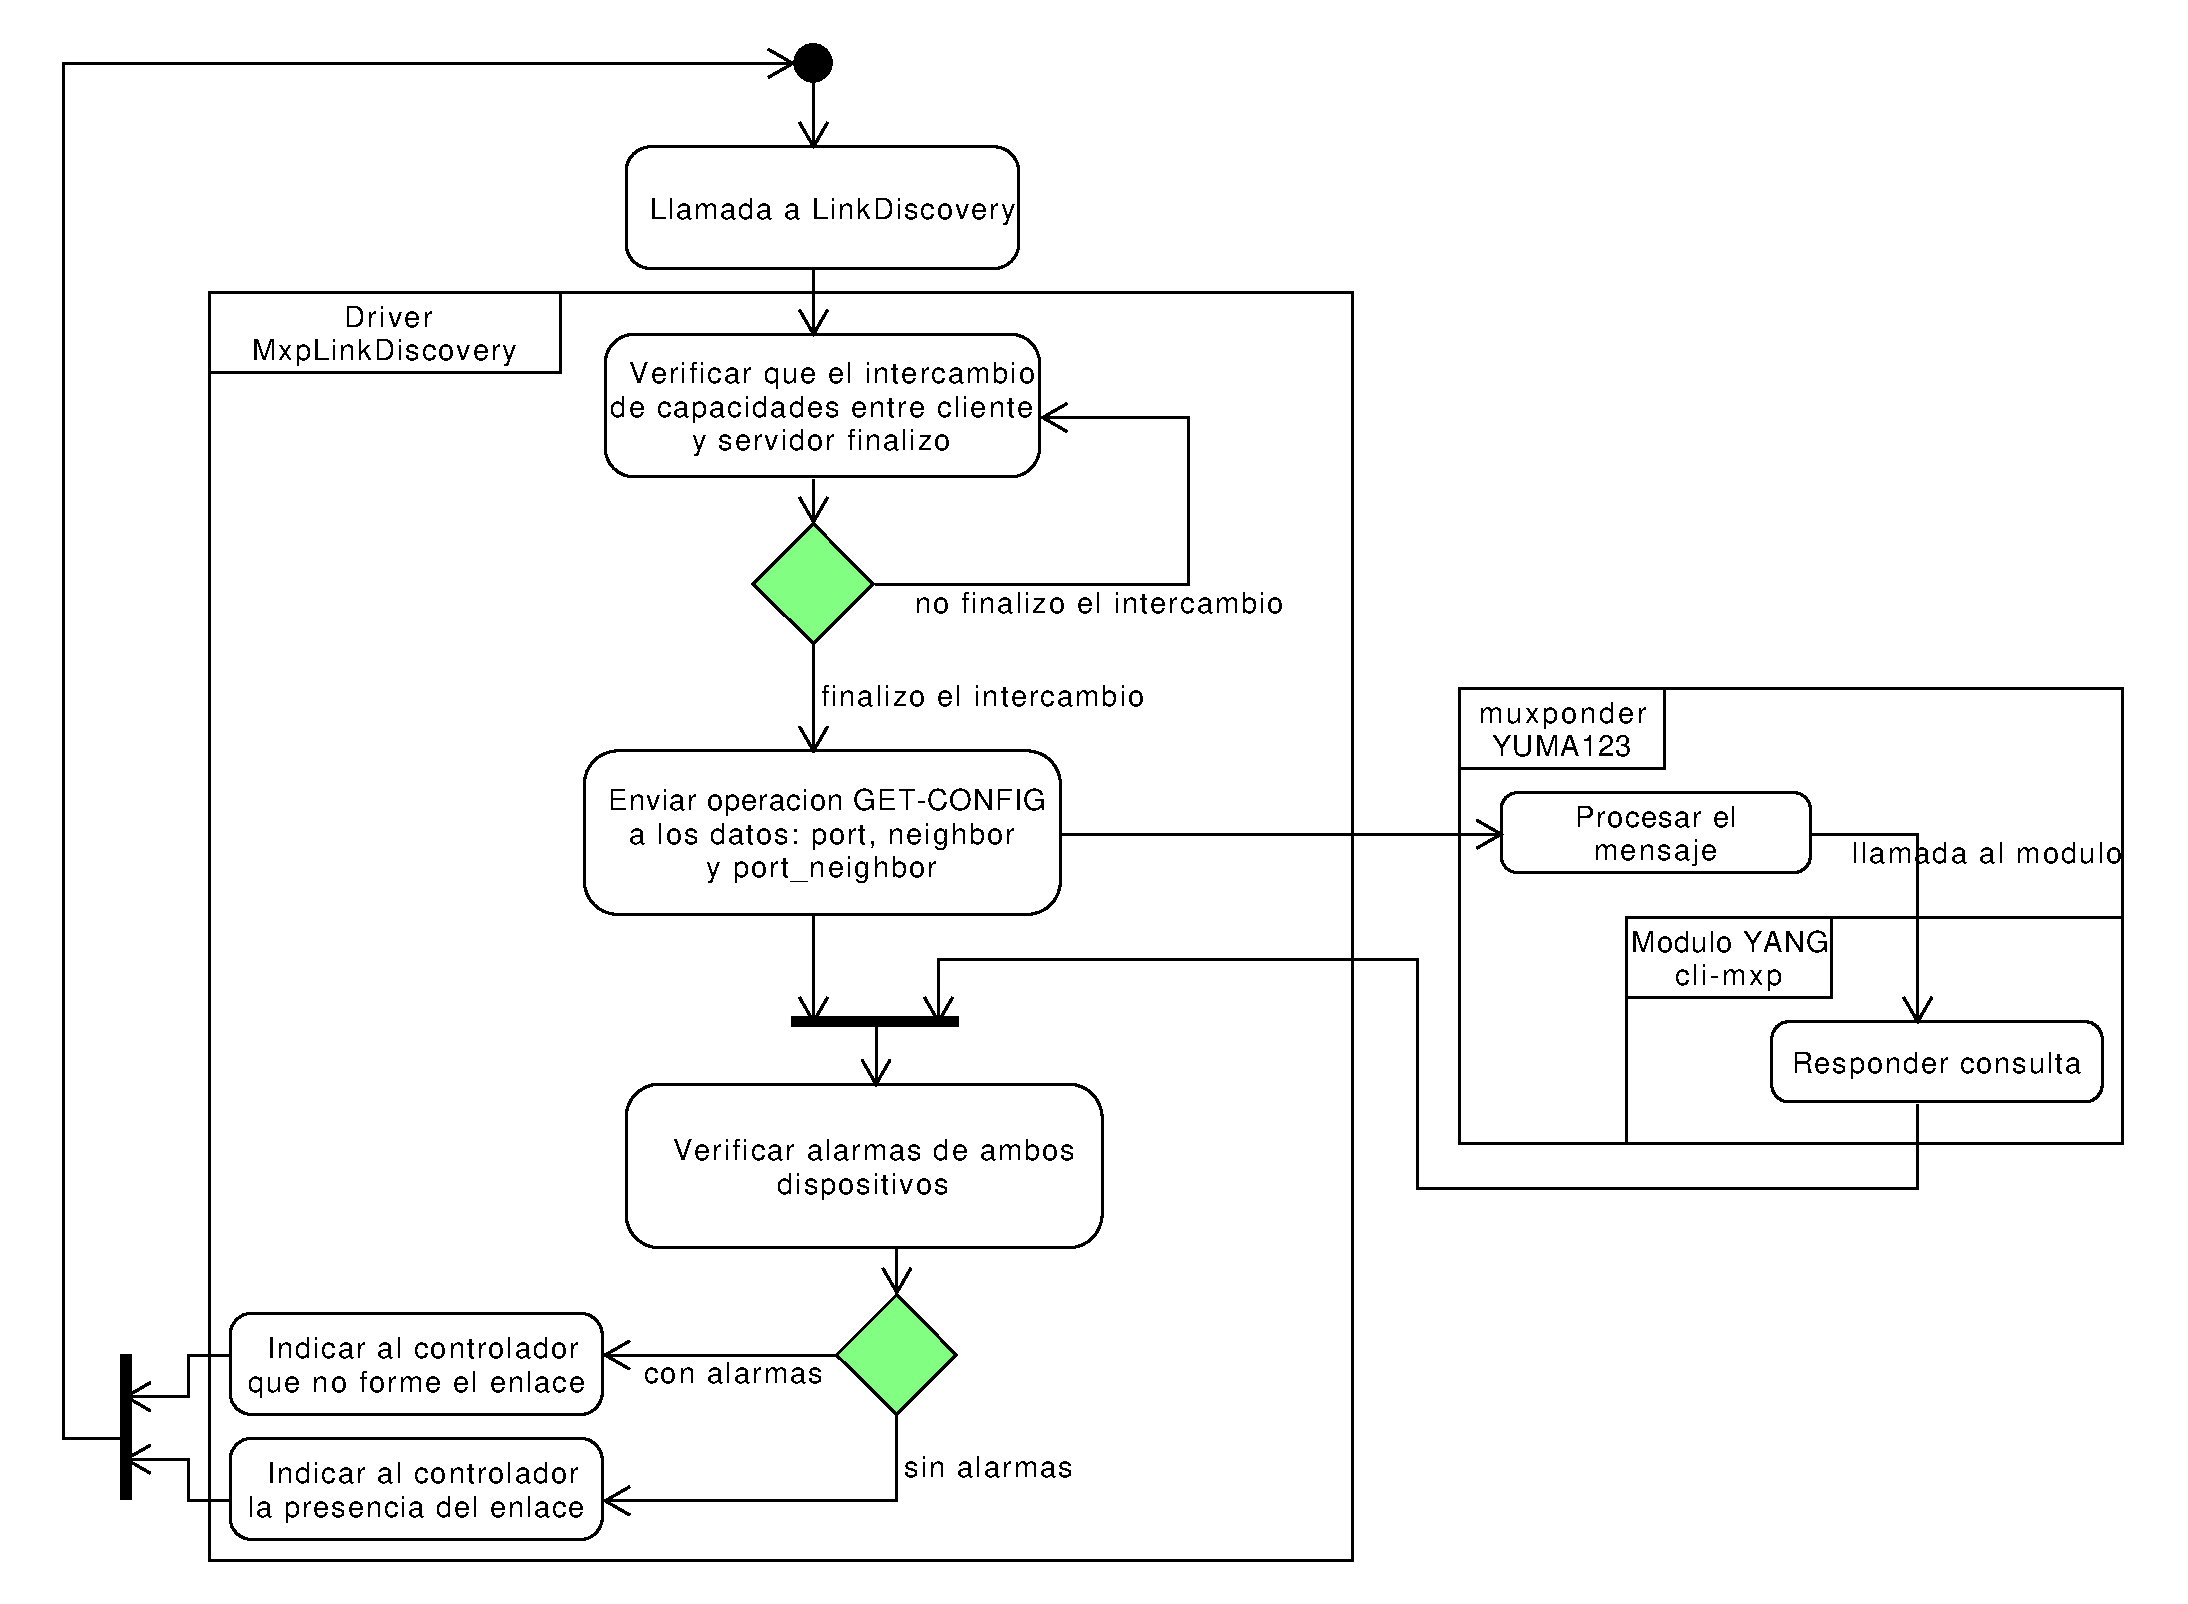
\includegraphics[scale=0.43]{Figures/actividad_link.pdf}
    \caption{Diagrama de actividad de la función \textit{LinkDiscovery}.}
    \label{fig:actividad_link}
  \end{figure}

  Es importante mencionar que en esta instancia, no se consulta al dispositivo por sus alarmas con un mensaje \textit{NETCONF} ya que las mismas son enviadas asíncronamente mediante notificaciones por el dispositivo, y registradas por el controlador como alarmas. Por lo tanto, para verificar el estado de las alarmas de un dispositivo solo se consulta internamente en el \textit{core} de \textit{ONOS}.

  \subsection{Operaciones definidas en el \textit{driver}} \label{drivermux}

  El \textit{driver} desarrollado brinda, además de las implementaciones de \textit{LinkDiscovery} y \textit{DeviceDescriptionDiscovery} explicadas anteriormente, la posibilidad de ejecutar cualquier operación admitida por el módulo del dispositivo, entre ellas la \textit{RPC} que se describió en el código \ref{lstlisting:RPC}. Se explica así el funcionamiento de la interfaz implementada para la operación \textit{RPC} 'mux-apply-config'. 
  \\

  Al momento de llamar a la función \textit{rpcApplyConfig}, la cual describe el comportamiento que tendrá la \textit{RPC} 'mux-apply-config' en el \textit{driver}, el mismo envía un mensaje al \textit{muxponder} solicitando que aplique la configuración que tiene el \textit{datastore running} haciendo uso del binario 'muxponder', tal como se mostró en la figura \ref{fig:actividad_modulo_sinc}.
  
  Luego, dado que se puede indicar la presencia de dispositivos vecinos, es necesario que el \textit{driver} corrobore que la configuración aplicada entre ellos sea la misma para garantizar la conectividad entre los clientes conectados a los \textit{muxponders}. Así, si se aplica una configuración en un \textit{muxponder}, el controlador deberá consultar y comparar la configuración que llevan los dispositivos vecinos. Si la configuración resulta ser la misma, no se genera ninguna alarma, de lo contrario se deberá generar y registrar una alarma en el controlador indicando una configuración inconsistente entre los dispositivos.
  \\

  Teniendo en cuenta esto, el diagrama de la figura \ref{fig:actividad_driver_rpc_sin_vecinos} muestra el flujo de actividad que sigue el \textit{driver} cuando recibe una llamada a 'mux-apply-config' para el \textit{muxponder} A. 
  En primer lugar, el \textit{driver} envía un mensaje al dispositivo con la operación \textit{RPC} que define el módulo \textit{YANG}. El agente Yuma123 recibe este mensaje, lo procesa y aplica la configuración en el equipo haciendo uso de los datos de configuración que tenga el \textit{datastore running}. Por último, se envía un mensaje con la respuesta de esa operación.  

  Luego, el \textit{driver} consulta al mismo \textit{muxponder} si tiene algún vecino conectado. Para este primer caso, el \textit{muxponder} A no tiene especificado ningún vecino, por lo que no se generará alguna alarma sobre configuración inconsistente, de hecho se verifica que no tenga alarmas de este tipo y de tenerlas se eliminan.


  \begin{figure}[H]
    \centering
    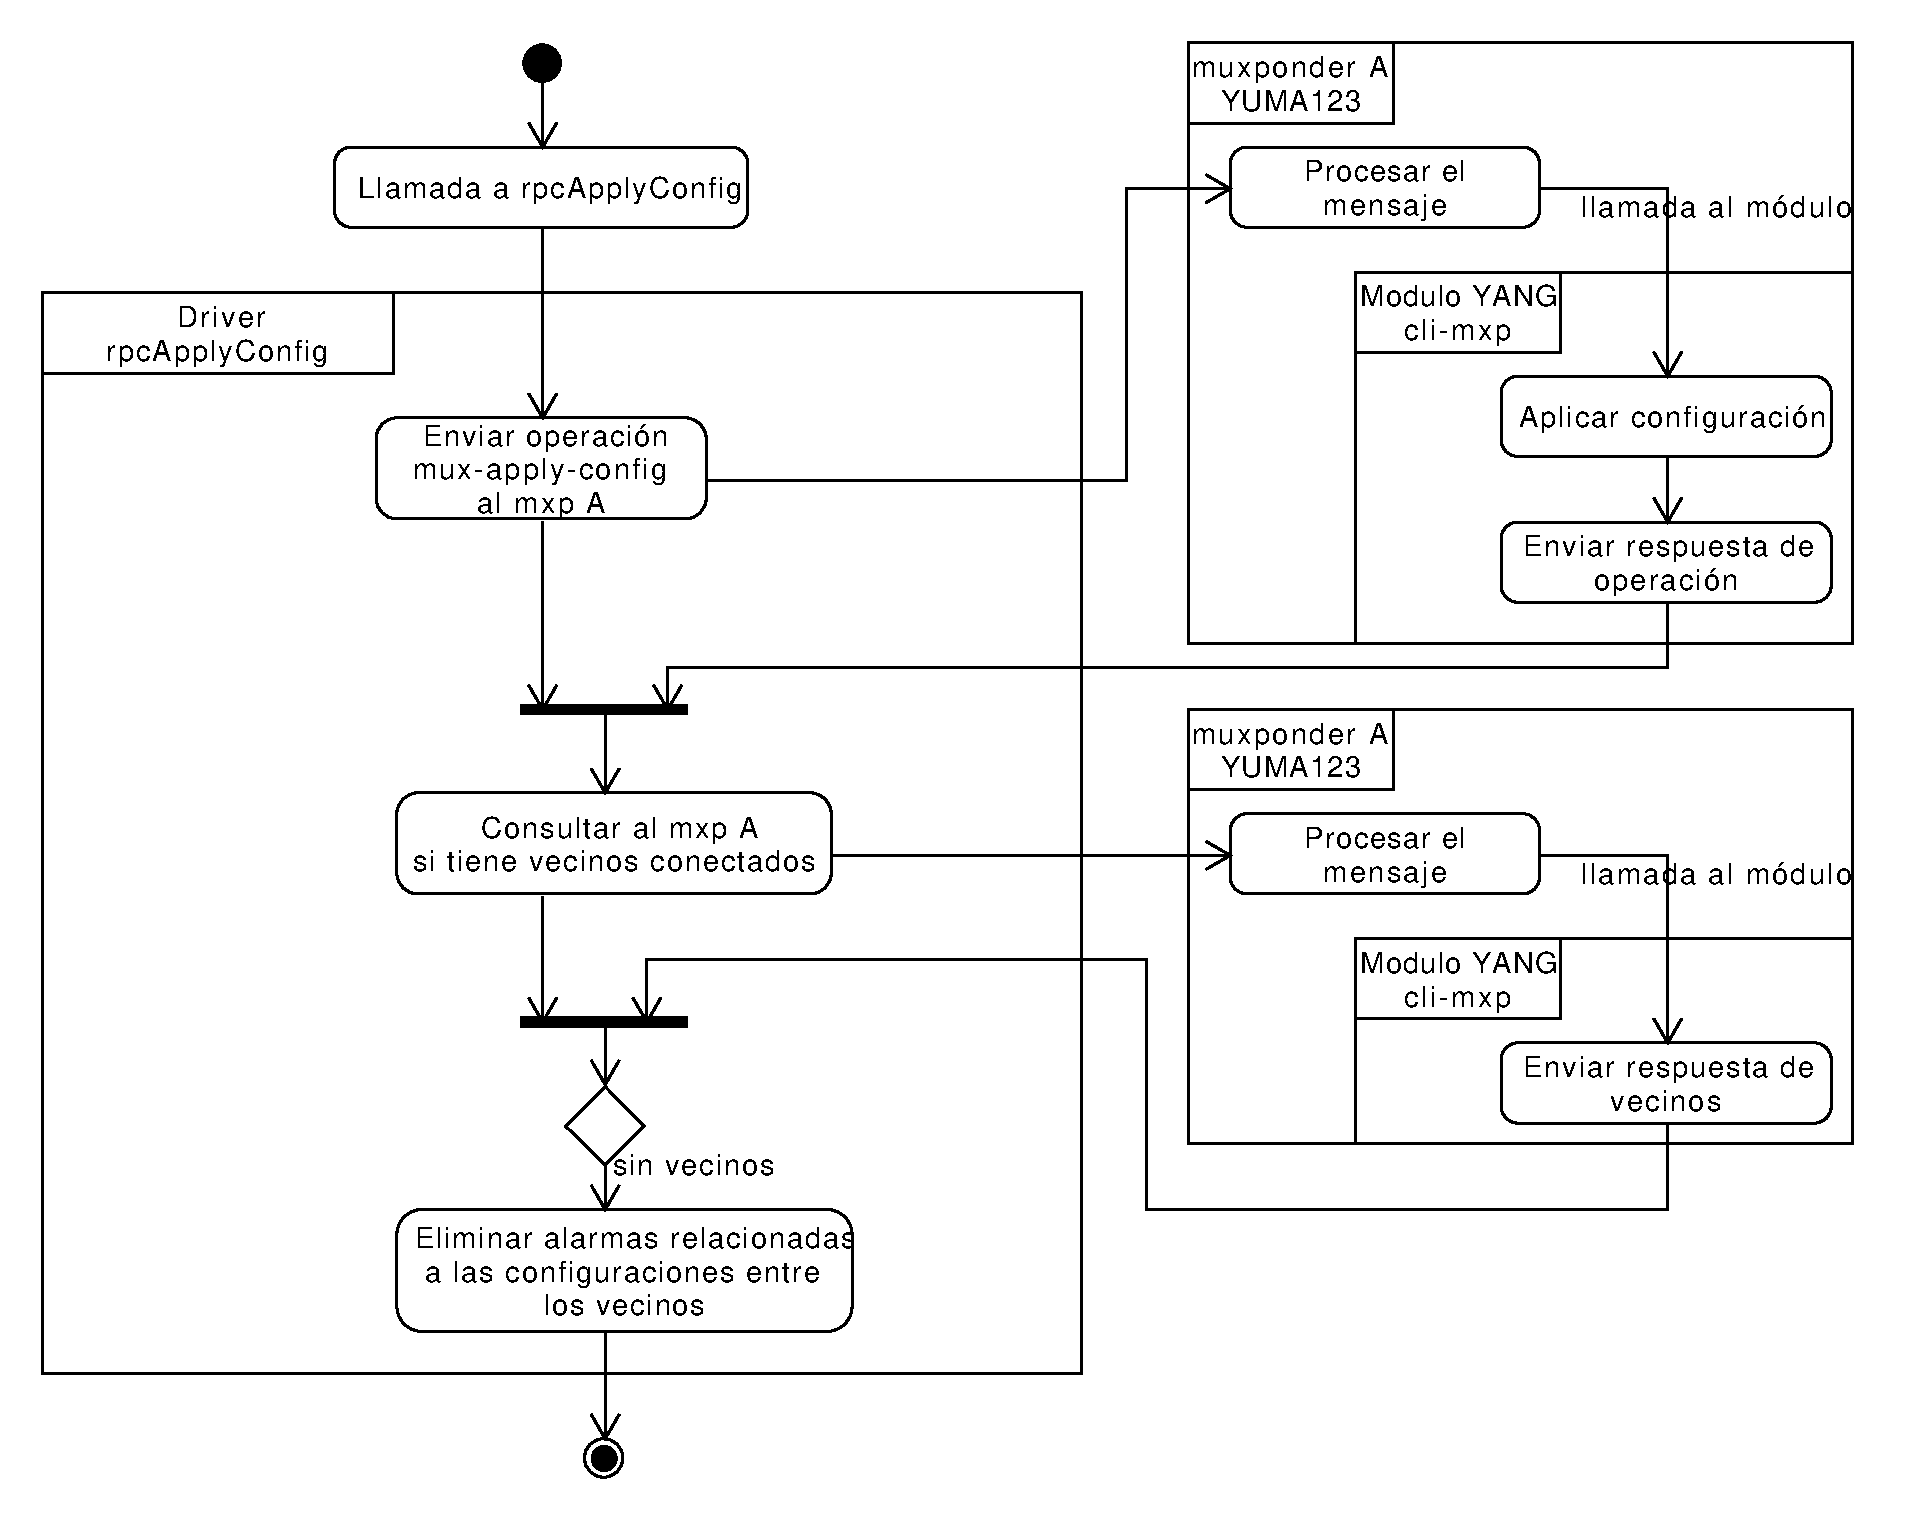
\includegraphics[scale=0.45]{Figures/actividad_driver_rpc_sin_vecinos.pdf}
    \caption{Diagrama de actividad para la \textit{RPC} 'mux-apply-config', sin vecinos.}
    \label{fig:actividad_driver_rpc_sin_vecinos}
  \end{figure}

  En caso de que el \textit{muxponder} A tenga vecinos conectados, el flujo de actividad es el que se muestra en la figura \ref{fig:actividad_driver_rpc_con_vecinos}. Se consulta al dispositivo vecino (\textit{muxponder} B) su configuración y se la compara con la configuración aplicada recientemente al dispositivo local (\textit{muxponder} A). Si las configuraciones resultan ser las mismas, se buscan las alarmas relacionadas a configuración inconsistente entre el \textit{muxponder} A y B, y de existir, se eliminan. Por el contrario, si la configuración es distinta, se crea una alarma y se la registra en el controlador.

  \begin{figure}[H]
    \centering
    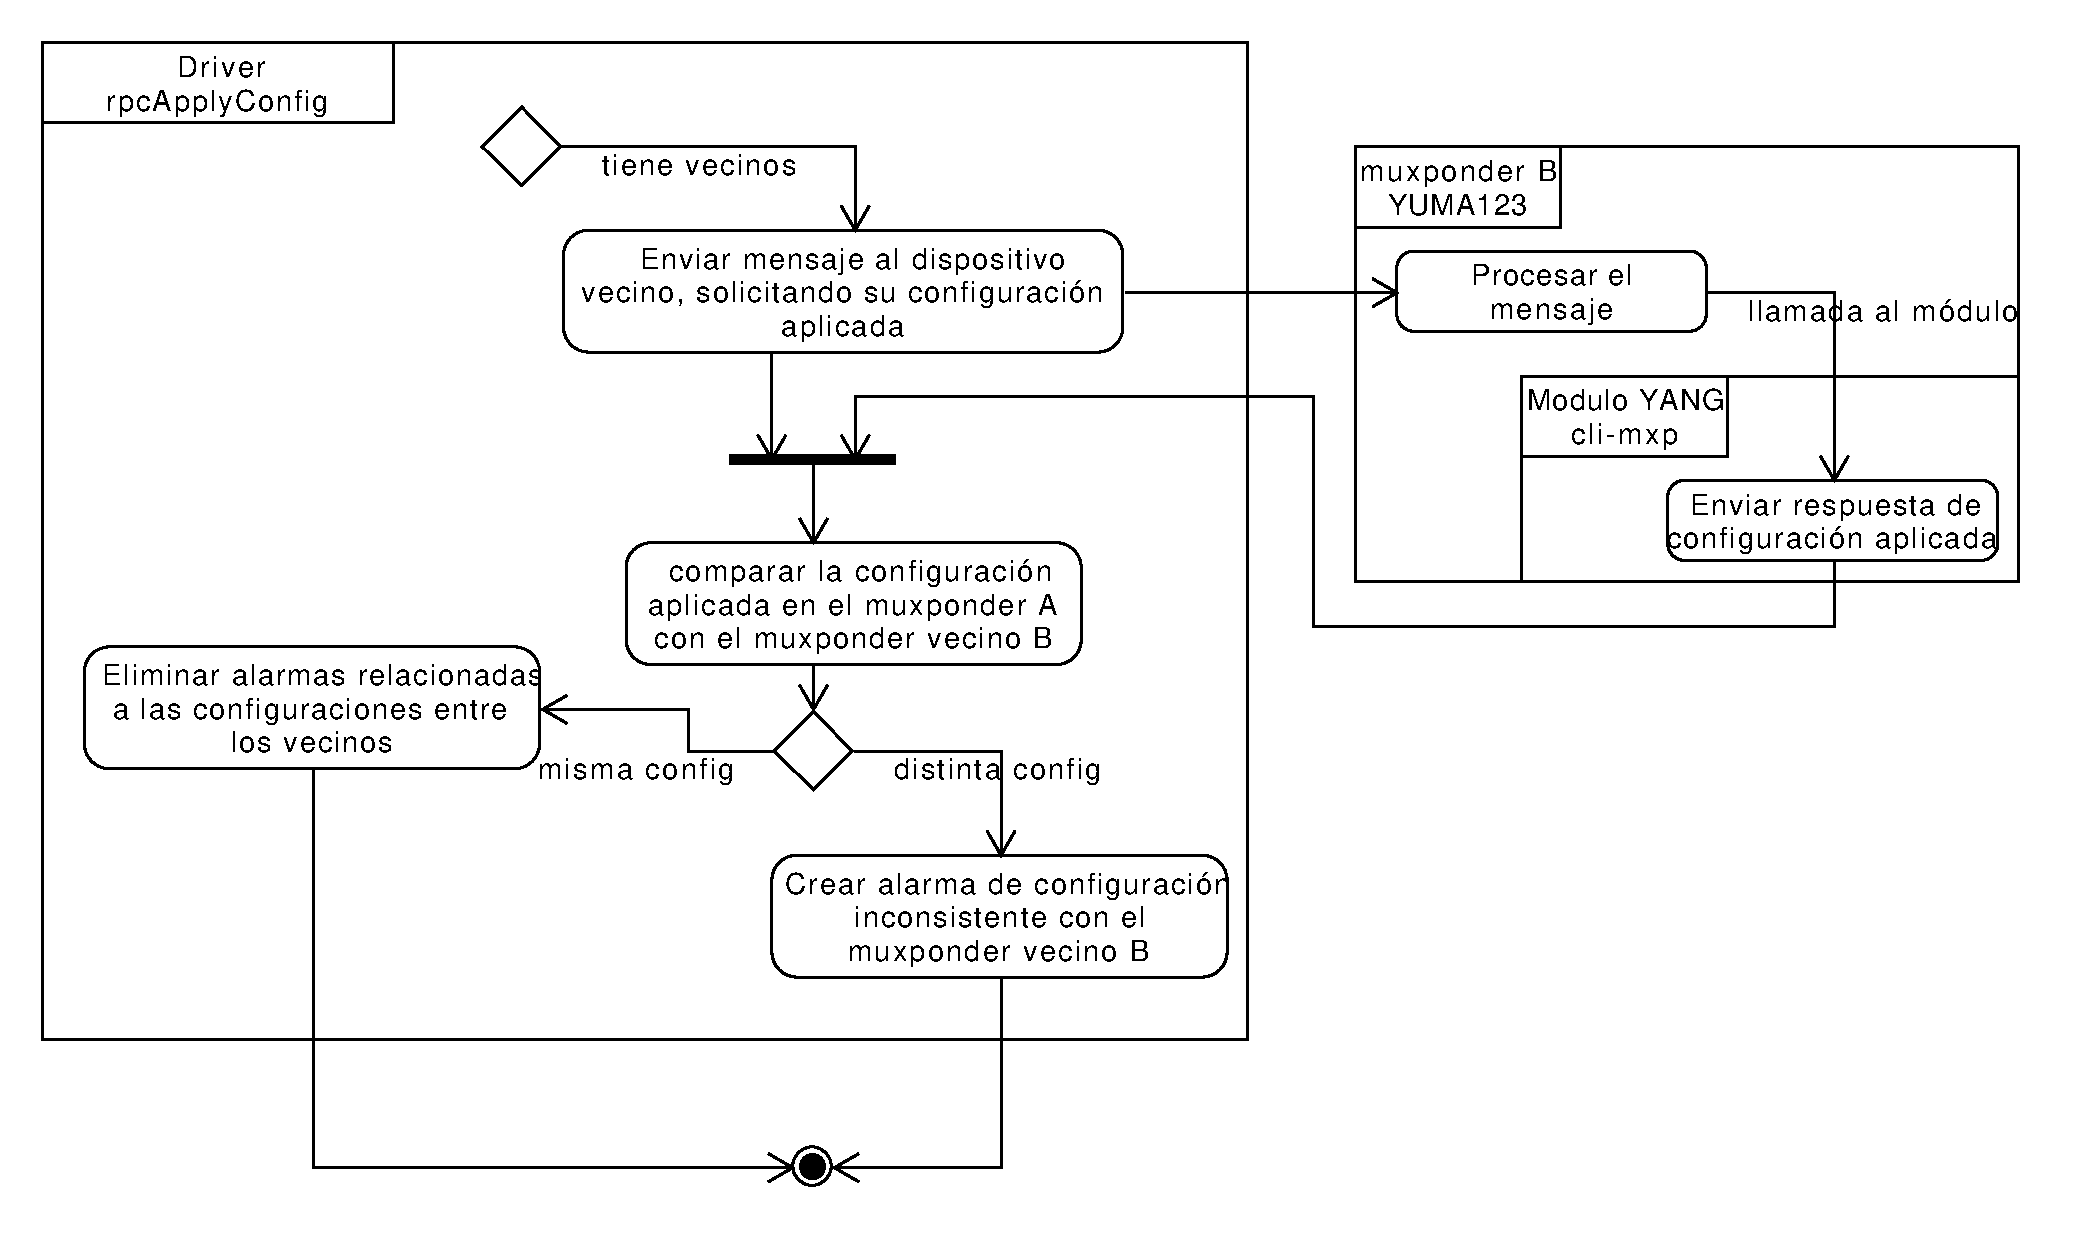
\includegraphics[scale=0.44]{Figures/actividad_driver_rpc_con_vecinos.pdf}
    \caption{Diagrama de actividad para la \textit{RPC} 'mux-apply-config', con vecinos.}
    \label{fig:actividad_driver_rpc_con_vecinos}
  \end{figure}


  Por último, es importante mencionar que con el fin de cumplir con el requerimiento R-14 de la figura \ref{fig:req_driver}, se implementaron comandos \textit{CLI} para que el administrador pueda interactuar con los dispositivos a través del \textit{driver}, haciendo uso de la consola de \textit{ONOS}. De esta forma, el administrador puede llamar a cualquiera de las funciones explicadas anteriormente, permitiéndole así poder gestionar la configuración de los dispositivos a través de la consola.

  \section{Diseño de la interfaz \textit{Northbound} e Interfaz de usuario}
  Para cumplir con los requerimientos del sistema, será necesario crear en primera instancia una interfaz \textit{REST API} a las aplicaciones externas, para que las mismas puedan comunicarse con los dispositivos administrados (\textit{muxponders}) por el controlador. Como se estudió en capítulos anteriores, \textit{ONOS} utiliza una interfaz llamada \textit{Northbound} para comunicarse con la capa de aplicación, y es aquí donde se encuentra implementada la aplicación \textit{REST}. 

  También, se deberá diseñar y crear una aplicación \textit{WEB} que sirva como interfaz de usuario al administrador, y a diferencia de la aplicación \textit{REST}, la \textit{GUI} desarrollada residirá en la capa de aplicación. La figura \ref{fig:ubicacionapp} esclarece la ubicación de las aplicaciones mencionadas anteriormente. 

  \begin{figure}[H]
    \centering
    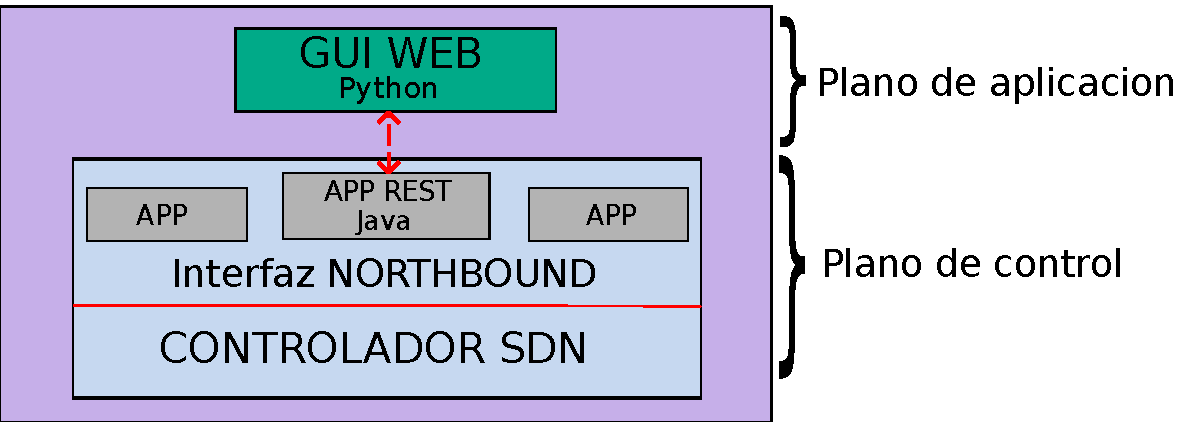
\includegraphics[scale=0.60]{Figures/arq-rest-gui.pdf}
    \caption{Interfaz \textit{REST} e interfaz de usuario.}
    \label{fig:ubicacionapp}
  \end{figure}

  \subsection{Requerimientos}

  A continuación, se listan en la figura \ref{fig:req_app} los diferentes requerimientos que deberán cumplir la interfaz \textit{REST} y la GUI. Los requerimientos R-15, R-16 y R-17 corresponden a la interfaz \textit{REST}, mientras que los requerimientos R-18 a R-21 pertenecen a la \textit{GUI} desarrollada.  

  \begin{figure}[!h]
    \centering
    \begin{subfigure}[b]{1\textwidth}
        \centering
        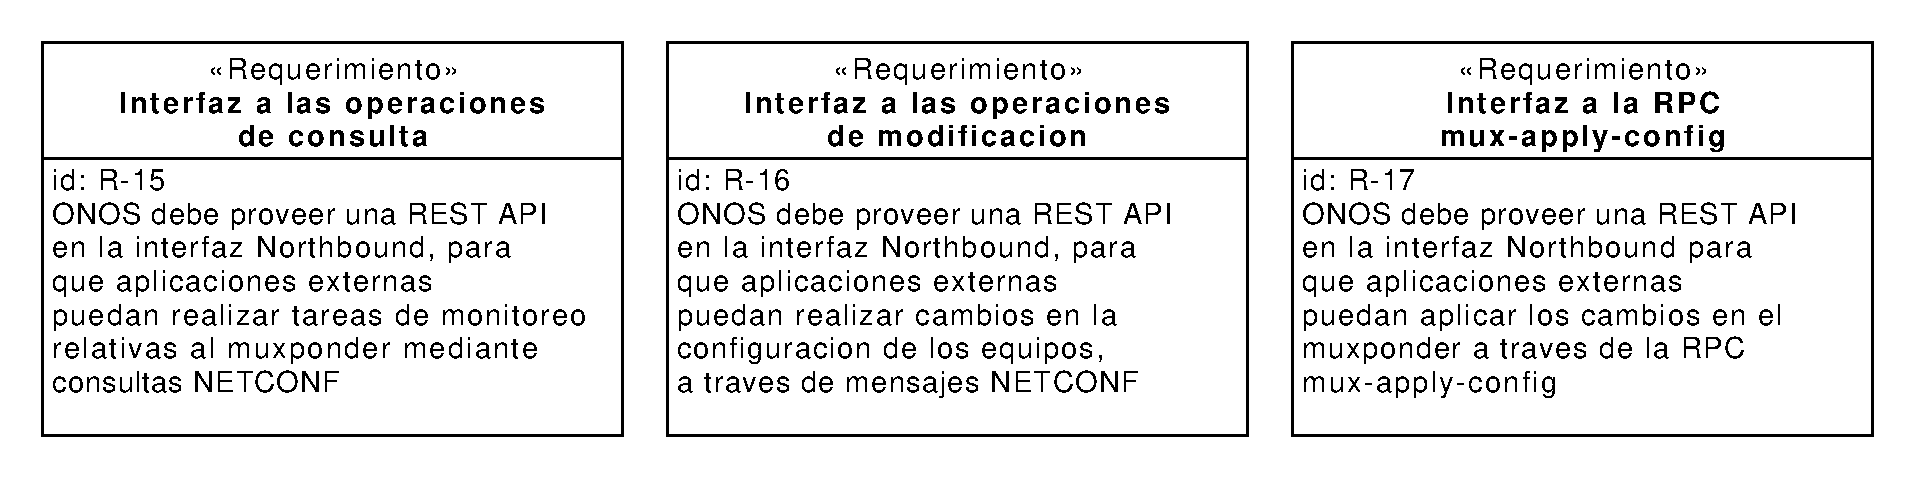
\includegraphics[width=\textwidth]{Figures/req_rest_rest.pdf}
        \caption{Requerimientos para la aplicación \textit{REST}.}
    \end{subfigure}
    \quad
    \vskip\baselineskip
    \begin{subfigure}[b]{0.75\textwidth}   
        \centering 
        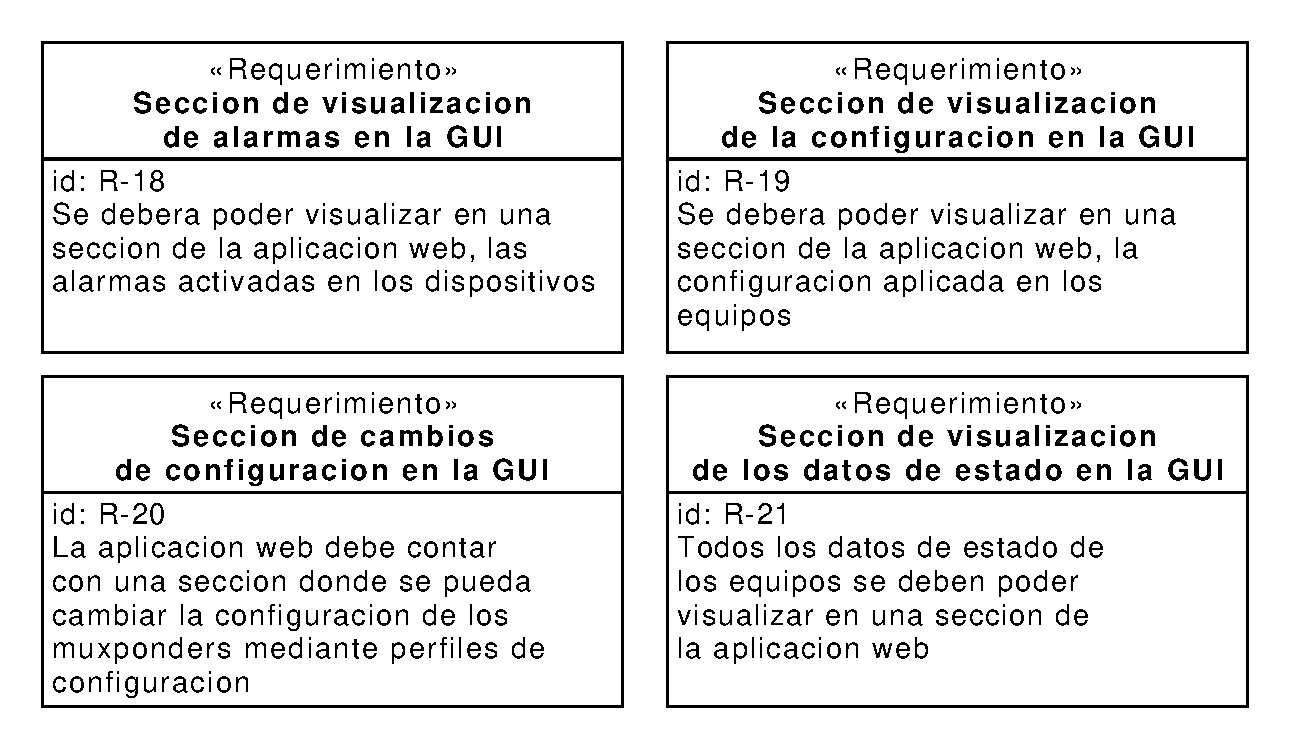
\includegraphics[width=\textwidth]{Figures/req_rest.pdf}
        \caption{Requerimientos para la aplicación \textit{WEB}.}
    \end{subfigure}
    \caption{Requerimientos de las interfaces REST e interfaz gráfica.}
    \label{fig:req_app}
\end{figure}



  \subsection{Implementación de la \textit{REST}}

  Para el desarrollo de la aplicación que se ejecuta en la interfaz \textit{Northbound} del controlador, se utilizó la herramienta \textit{onos-create-app} \parencite{onosapptemplate}. La misma, crea un esqueleto de una aplicación simple con una interfaz \textit{REST}, a partir de la cual se realizaron modificaciones para poder cumplir con los requerimientos R-15, R-16 y R-17.

  Así, la aplicación \textit{REST API} se encuentra dividida en cinco clases de Java, las cuales se detallan a continuación. 


  \begin{itemize}
	\item \textbf{AppComponent}: esta clase resulta del uso de la herramienta \textit{onos-create-app}. Aquí se define el comportamiento que tendrá la aplicación al momento de su activación y desactivación. En este caso, cuando se activa la aplicación en el controlador, la misma inicia un objeto \textit{Listener} para poder imprimir mensajes de log y \textit{debbug}.
    
    \item \textbf{AppWebApplication}: también resulta del uso de la aplicación mencionada anteriormente. El objetivo de esta clase, es la de indicar cuáles serán las funciones de la aplicación que serán expuestas en la \textit{Northbound} interface de \textit{ONOS}.

    \item \textbf{GetWebResource}: en esta clase se definen las operaciones de consulta que son expuestas, a través de la clase \textit{AppWebApplication}, a la interfaz \textit{Northbound} del controlador. En ella, se definen funciones que tienen operaciones GET de HTTP, las cuales aceptan ciertos parámetros dependiendo de la operación (por ejemplo, indicar a qué dispositivo se quiere realizar la consulta). Seguidamente, la función llama al \textit{driver} del dispositivo con los parámetros que recibió,  y devuelve una respuesta a las aplicaciones que la llamaron.
    
    \item \textbf{RpcWebResource}: de forma similar, esta clase expone una interfaz \textit{REST API} a la \textit{RPC} 'mux-apply-config' definida en el módulo \textit{YANG}. Así, las aplicaciones externas especifican el id de un dispositivo, para que luego la interfaz \textit{REST} se comunique con el mismo mediante el \textit{driver} desarrollado. 
    
    \item \textbf{SetWebResource}: por último, se expone una interfaz con operaciones PUT de HTTP, con las cuales se posibilita que las aplicaciones externas puedan realizar cambios en las bases de datos \textit{running}, \textit{candidate} o \textit{startup} de los dispositivos.

\end{itemize}

Se muestra en la figura \ref{fig:rest_capt} un ejemplo de la interfaz \textit{REST}. En la misma, se puede observar las diferentes operaciones expuestas explicadas anteriormente.

\begin{figure}[H]
    \centering
    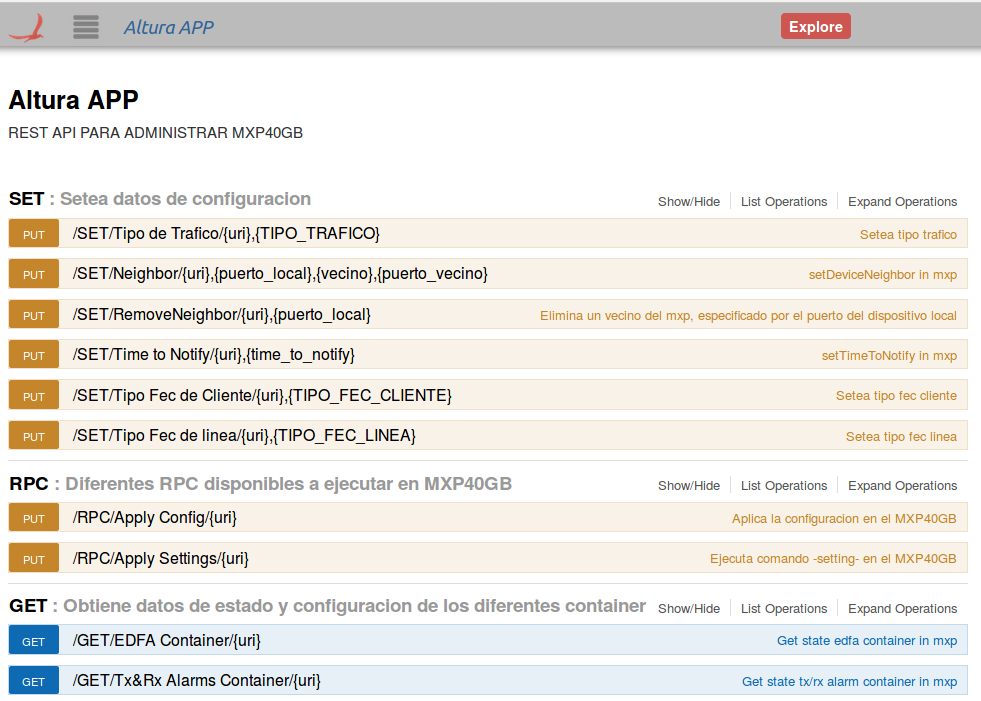
\includegraphics[scale=0.41]{Figures/captura-rest.png}
    \caption{Fragmento de la interfaz \textit{REST} implementada.}
    \label{fig:rest_capt}
  \end{figure}


  \subsection{Implementación de la interfaz de usuario}
  A fin de cumplir con los requerimientos R-18 a R-21 de la figura \ref{fig:req_app}, se realizó una aplicación \textit{WEB} basada en el \textit{microframework} Flask \parencite{flask}. La misma, se desarrolla en Python y hace uso de lenguajes como HTML, JavaScript y CSS para presentar la interfaz de usuario. Cada sección listada en los requerimientos de la figura \ref{fig:req_app} (B), corresponde a un archivo HTML que contiene la estructura de la aplicación y los datos que se presentan en la interfaz. 

Es importante mencionar que todas las vistas realizan una tarea común. Dicha tarea consiste en consultar periódicamente al controlador las alarmas activas que tiene \textit{ONOS} relativas a los \textit{muxponders}. Se puede observar el diagrama de actividad de la tarea mencionada en la figura \ref{fig:consulta_alarmas}.

\begin{figure}[H]
    \centering
    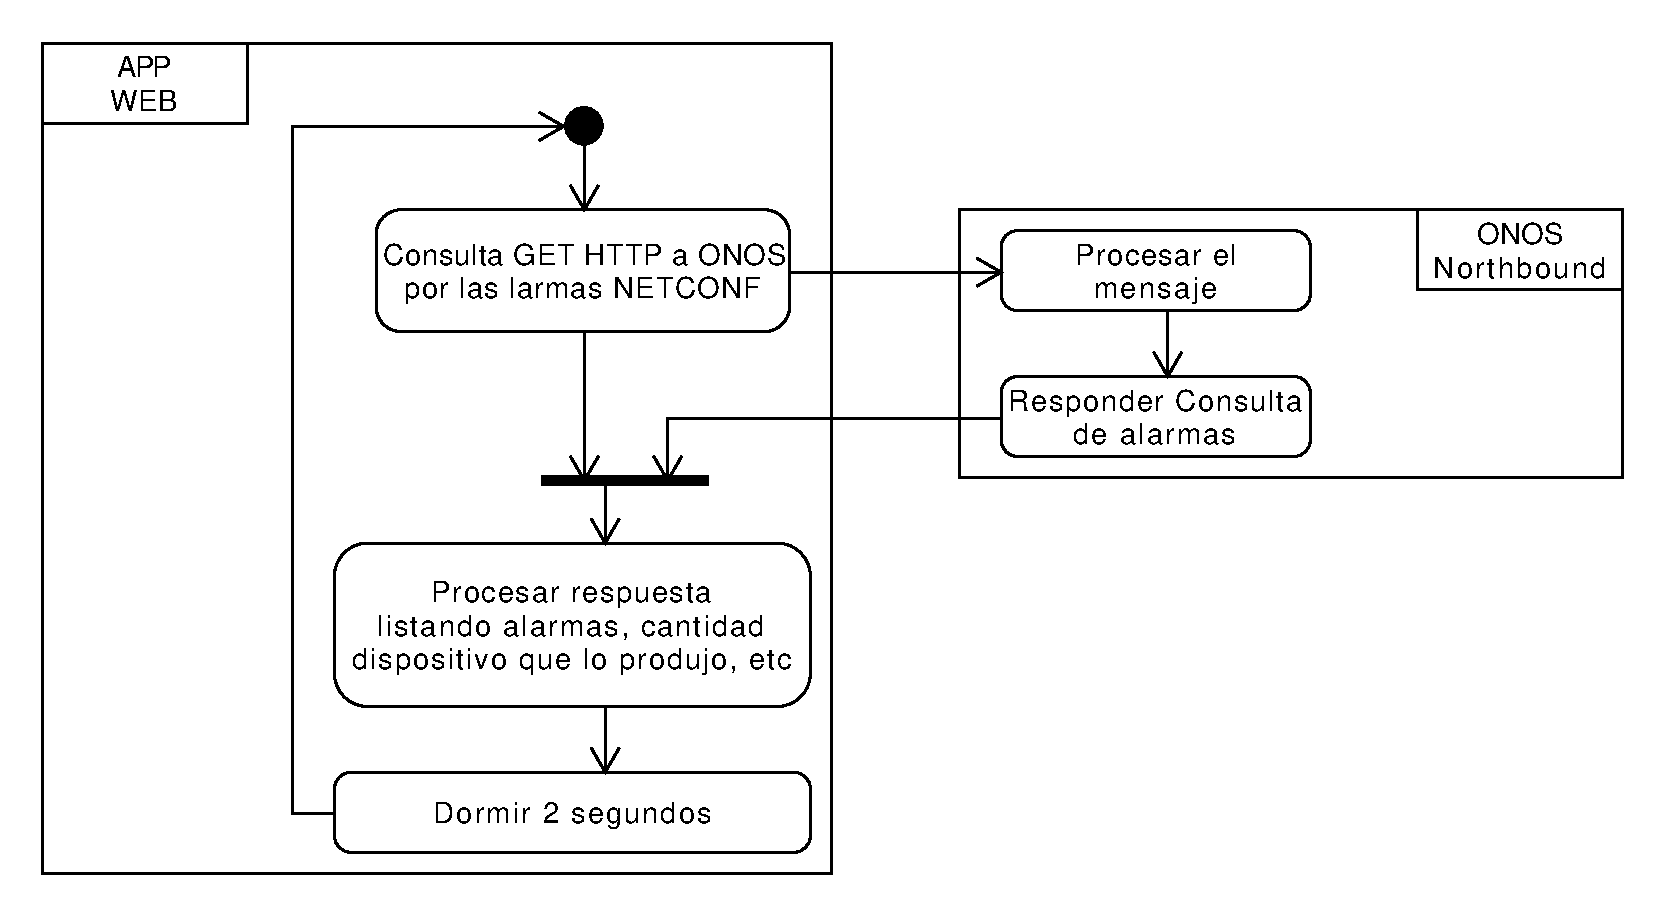
\includegraphics[scale=0.45]{Figures/consulta_alarmas.pdf}
    \caption{Consulta periódica por las alarmas al controlador \textit{ONOS}.}
    \label{fig:consulta_alarmas}
  \end{figure}

  Como ya se explicó en este capítulo, las alarmas son enviadas por los dispositivos a través de las notificaciones \textit{NETCONF}. Luego, el controlador las registra internamente, por lo que no es necesario hacer uso de la interfaz \textit{Southbound} para consultar a los equipos por el estado de las alarmas. De esta forma, los mismos se ven aliviados al no tener que procesar periódicamente estas consultas.
  \\

  Teniendo en cuenta esta actividad común, el desarrollo de la \textit{GUI} se divide en las siguientes secciones:

  \begin{itemize}
	\item \textbf{Vista principal}: tal como se puede observar en la figura \ref{fig:captura_web_principal}, esta vista muestra la cantidad de la alarmas presentes en el controlador, sin entrar en detalles. A su vez, en la parte inferior se permite agregar nuevos dispositivos a la topología, indicando la dirección IP y el puerto. Por último, en la zona superior se brinda un campo donde puede seleccionarse un conjunto de equipos para posteriormente aplicar una configuración con un perfil dado. 

    \begin{figure}[H]
        \centering
        \resizebox{\textwidth}{!}{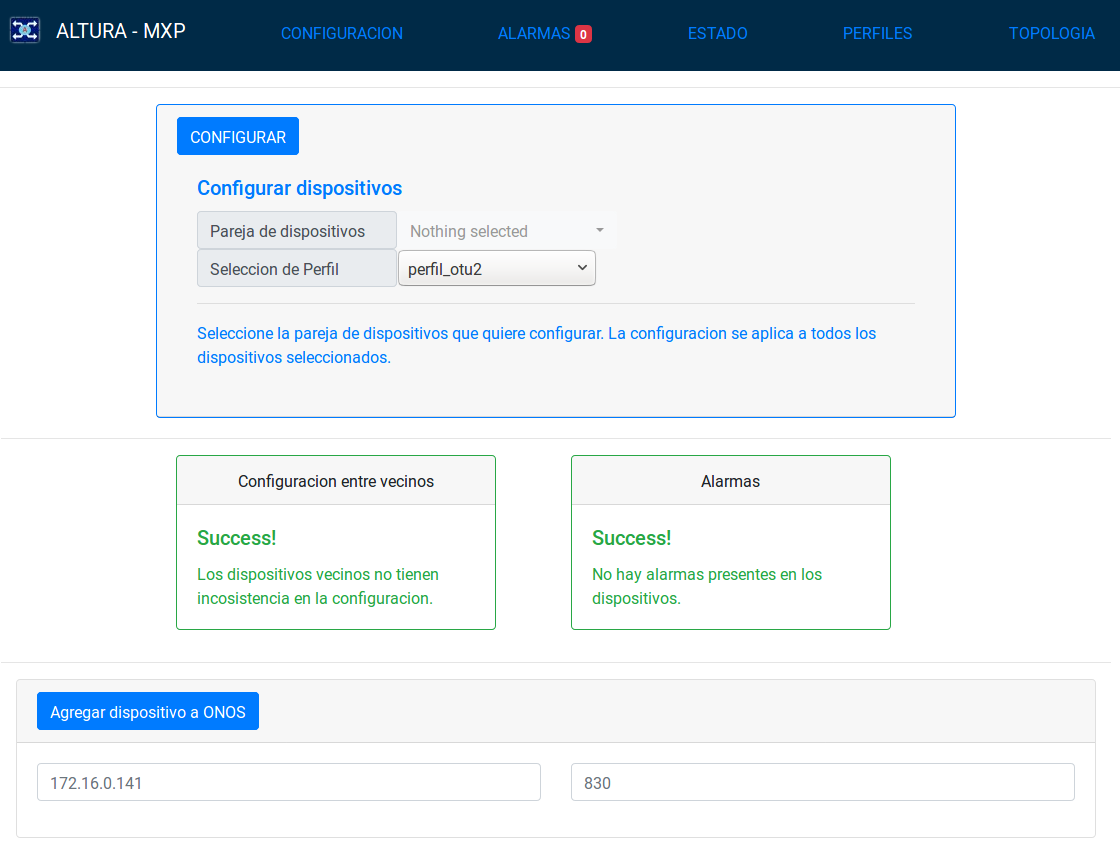
\includegraphics{Figures/vista_principal.png}}
        \caption{Interfaz de la vista principal.}
        \label{fig:captura_web_principal}
      \end{figure}

    Por otra parte, en el diagrama de la figura \ref{fig:agregar_disp_web} se muestra cómo la aplicación \textit{WEB} conforma un mensaje JSON con la información del equipo (dirección IP, puerto) y la envía al controlador a través de la interfaz\textit{ REST}. Finalmente, el controlador procesa el mensaje dando inicio al descubrimiento del dispositivo. 

    \begin{figure}[H]
        \centering
        \includegraphics[scale=0.45]{Figures/agregar_disp_web.pdf}
        \caption{Agregar dispositivo a través de la APP \textit{WEB}.}
        \label{fig:agregar_disp_web}
      \end{figure}

    Por último, la figura \ref{fig:config_disp_web} muestra como es el proceso de configuración de un \textit{muxponder} a través de la aplicación WEB. Primeramente, se envía el perfil de configuración. Una vez que la información es almacenada en el \textit{datastore running}, se envía la \textit{RPC} 'mux-apply-config' para que se apliquen los cambios en el dispositivo.

    \begin{figure}[H]
        \centering
        \includegraphics[scale=0.45]{Figures/config_disp_web.pdf}
        \caption{Configurar un dispositivo a través de la APP \textit{WEB}.}
        \label{fig:config_disp_web}
      \end{figure}

    \item \textbf{Vista de alarmas}:  la figura \ref{fig:captura_web_alarmas} detalla el contenido de dicha sección. Aquí se muestra una información más detallada de las alarmas. El administrador puede identificar el tipo de alarma, el dispositivo que lo originó y la cantidad de alarmas totales que presenta la topología. El diagrama de actividad que refleja el comportamiento que realiza la interfaz \textit{WEB} en esta sección, se mostró en la figura \ref{fig:consulta_alarmas}.
   
    \begin{figure}[H]
        \centering
        \resizebox{\textwidth}{!}{\includegraphics{Figures/vista_alarmas.png}}
        \caption{Interfaz de la vista de alarmas.}
        \label{fig:captura_web_alarmas}
      \end{figure}
    
    \item \textbf{Vista de datos de configuración}: la interfaz que muestra la misma es la que se observa en la figura \ref{fig:captura_web_config}. Presenta así una sección donde se puede observar una lista de los equipos que conforman la topología con sus respectivas configuraciones aplicadas. 
        
    \begin{figure}[H]
        \centering
        \resizebox{\textwidth}{!}{\includegraphics{Figures/vista_config.png}}
        \caption{Interfaz de la vista de configuración.}
        \label{fig:captura_web_config}
      \end{figure}

    \item \textbf{Vista de datos de estado}: a continuación, se muestra la figura \ref{fig:captura_web_estado} la interfaz que presenta dicha vista. De forma similar a la anterior, aquí se muestra información relacionada a los datos de estado de los equipos. En la parte superior se puede observar los diferentes \textit{containers} de estado que se implementaron en el módulo \textit{YANG}.  
    
    \begin{figure}[H]
        \centering
        \resizebox{\textwidth}{!}{\includegraphics{Figures/vista_estado.png}}
        \caption{Interfaz de la vista de estado.}
        \label{fig:captura_web_estado}
      \end{figure}

    \item \textbf{Vista de topología}: tal como se observa en la figura \ref{fig:captura_web_topo}, aquí se permite realizar cambios en la topología de la red a través de mensajes \textit{NETCONF} a los dispositivos. Así, se puede especificar una pareja de equipos para que el controlador, mediante la función \textit{LinkDiscovery}, pueda formar o eliminar los enlaces entre los mismos.
    
    \begin{figure}[H]
        \centering
        \resizebox{\textwidth}{!}{\includegraphics{Figures/vista_topo.png}}
        \caption{Interfaz de la vista de topología.}
        \label{fig:captura_web_topo}
      \end{figure}
    
    \item \textbf{Vista de perfiles}: por último, en la figura \ref{fig:captura_web_topo} se presenta una sección donde se permite agregar o eliminar perfiles de configuración. La idea básica de los perfiles de configuración es la de agrupar una serie de parámetros de tal forma que el administrador pueda identificar fácilmente cuál será la configuración que se aplique en el dispositivo. Además, permite guardar dicho perfil con el fin de poder reutilizarlo en un futuro. 

    \begin{figure}[H]
        \centering
        \resizebox{\textwidth}{!}{\includegraphics{Figures/vista_perfiles.png}}
        \caption{Interfaz de la vista de administración perfiles de configuración.}
        \label{fig:captura_web_topo}
      \end{figure}
    
\end{itemize}



% \subsubsection*{Casos de uso}

 % Chapter Template

\chapter{Diseño e Implementación} % Main chapter title
% cSpell:words resizebox \textit{onosapi} usecase Mcast enrutamiento parencite includegraphics pcktprocactiv lstlisting iperf

\label{Chapter5} % Change X to a consecutive number; for referencing this chapter elsewhere, use 
% \ref{ChapterX} 
Para el desarrollo del proyecto será necesario implementar un sistema donde se puedan realizar pruebas y evaluar la correctitud del mismo. 

De esta forma, la primera sección de este capítulo comprende tanto el análisis del sistema como la topología utilizada. Específicamente, se estudiará su estructura, su comportamiento y sus requerimientos. 

En las secciones siguientes, se detallarán las aplicaciones desarrolladas que permiten cumplir con el objetivo del proyecto. En primer lugar, se hará un estudio del módulo \textit{YANG} implementado, el cual caracteriza y modela los datos del equipo. A continuación, se detallará el \textit{driver} implementado para lograr la comunicación entre el controlador y el dispositivo. Por último, se analizará la interfaz \textit{REST} y la \textit{GUI} desarrollada.

%----------------------------------------------------------------------------------------
%	SECTION 1
%----------------------------------------------------------------------------------------

\section{Entorno de trabajo}
En esta sección se detallan las características del sistema a implementar, descriptas en el lenguaje de especificación de sistemas SysML \parencite{sysml}. Se optó por este lenguaje de modelado ya que brinda una extensión a UML permitiendo combinar elementos del mundo físico (\textit{hardware}) con elementos del mundo lógico (\textit{software}). 

%-----------------------------------
%	SUBSECTION 1
%-----------------------------------

\subsection{Topología}

Se conformará una topología con el fin de poder identificar en una primera instancia, los requerimientos que debe cumplir el sistema. La misma, está basada en un caso de uso simple, en el cual se quiere brindar conectividad a dos clientes a través de un enlace óptico, este último conformado por dos \textit{muxponders}.  

Es importante identificar la presencia del controlador \textit{ONOS}, el cual gestionará la configuración de los equipos mediante el protocolo \textit{NETCONF}. En la figura \ref{fig:topologia} se muestra de forma general la topología planteada. 

Los dispositivos terminales A y B, se encuentran conectados al puerto cliente del \textit{muxponder} C y D, respectivamente. A su vez, el transmisor del \textit{muxponder} C se encuentra conectado al receptor del \textit{muxponder} D, y viceversa. Esto permite una comunicación bidireccional, donde ambos clientes pueden tener conectividad. 

Por otra parte, el controlador tiene una conexión con los \textit{muxponder} a través de los puertos de control de los mismos. 

\begin{figure}[H]
    \centering
    \includegraphics[scale=0.68]{Figures/topologia.pdf}
    \caption{Topología implementada en el proyecto.}
    \label{fig:topologia}
  \end{figure}


En la figura \ref{fig:topologiafis} se presenta cómo está dispuesta la conexión física de los equipos. En ella, se puede observar la alimentación de los equipos, los puertos clientes los cuales estarán conectados a los \textit{host} A y B antes mencionados. También, se observa las interfaces de línea conectadas entre sí, de tal manera que se permita una comunicación bidireccional entre los clientes. Por otro lado, las interfaces de control se conectan al controlador \textit{ONOS} tal cómo se mencionó anteriormente. 

\begin{comment}
A continuación, en la figura \ref{fig:topologiafis} se muestra como está dispuesta la conexión físicamente en los dispositivos. A la izquierda se tiene el \textit{muxponder} C, y a la derecha se encuentra el \textit{muxponder} D. Las interfaces de control de ambos dispositivos están conectadas al controlador \textit{ONOS}, mientras que los puertos clientes se encuentran conectados a los clientes A y B respectivamente. Por otra parte, las interfaces de línea se encuentran conectados entre los \textit{muxponder}, como se explicó anteriormente, con el fin de poder tener una comunicación bidireccional.
\end{comment}


\begin{figure}[H]
    \centering
    \resizebox{\textwidth}{!}{\includegraphics[scale=0.1]{Figures/mxpfisicos-min.pdf}}
    \caption{Conexión física de la topología.}
    \label{fig:topologiafis}
  \end{figure}


%-----------------------------------
%	SUBSECTION 2
%-----------------------------------
\subsection{Requerimientos del sistema}

Para establecer los requerimientos funcionales del sistema, se presentará en primer lugar un diagrama de caso de uso. Como se puede observar en la figura \ref{fig:caso_uso_admin}, el objetivo principal del sistema es poder brindar al administrador un entorno donde pueda gestionar la configuración de los \textit{muxponders} mediante sus aplicaciones.

\begin{figure}[H]
    \centering
    \includegraphics[scale=0.53]{Figures/caso_uso_admin.pdf}
    \caption{Caso de uso desde la perspectiva del administrador.}
    \label{fig:caso_uso_admin}
  \end{figure}

  En base a este diagrama, se pueden definir los requerimientos funcionales a nivel de sistema. La figura \ref{fig:req_sys} muestra una lista de los mismos. 
  
  Como requerimiento no funcional, se puede identificar la adición de nodos virtuales, los cuales no afectan a la funcionalidad del sistema pero brindan más flexibilidad y permiten conformar una topología más compleja.

  \begin{figure}[H]
    \centering
    \includegraphics[scale=0.65]{Figures/req_sys.pdf}
    \caption{Requerimientos del sistema.}
    \label{fig:req_sys}
  \end{figure}


  Además, a partir del diagrama de caso de uso de la figura \ref{fig:caso_uso_admin}, se pueden identificar tres diagramas de actividades relacionadas. La figura \ref{fig:actividad_config}, muestra los flujos de actividad típicos que tendrá el sistema. 
  
  Para la actividad relacionada al monitoreo \ref{fig:actividad_config} (A), la aplicación \textit{WEB} realiza consultas periódicas al controlador con el fin de obtener información sobre los dispositivos. Así, se envía un mensaje HTTP con la operación GET desde la aplicación, el controlador procesa la petición y responde dicha consulta.

Por otra parte, para el flujo de actividad relacionado a las notificaciones que puede verse en la figura \ref{fig:actividad_config} (B), es el dispositivo quien emite inicialmente el mensaje mediante una notificación \textit{NETCONF}. En el controlador se procesa la notificación y se la registra como alarma.

Por último, se tiene el diagrama de actividad relacionado a la configuración del equipo \ref{fig:actividad_config} (C). El evento inicial para este caso, es la adición de una configuración desde la aplicación \textit{WEB}. Dicha configuración, una vez procesada se traduce en una solicitud POST HTTP que se envían hacia la \textit{Northbound interface} del controlador. Una vez recibida la solicitud, se realiza su procesamiento y se envía el mensaje de configuración \textit{NETCONF} a los dispositivos involucrados a través de la \textit{Southbound interface}.


  


  \begin{figure}[!h]
    \centering
    \begin{subfigure}[b]{0.43\textwidth}
        \centering
        \includegraphics[width=\textwidth]{Figures/actividad_monitoreo.pdf}
        \caption{Actividad de monitoreo.}
    \end{subfigure}
    \quad
    \begin{subfigure}[b]{0.43\textwidth}  
        \centering 
        \includegraphics[width=\textwidth]{Figures/actividad_notif.pdf}
        \caption{Actividad de notificación.}
    \end{subfigure}
    \vskip\baselineskip
    \begin{subfigure}[b]{0.43\textwidth}   
        \centering 
        \includegraphics[width=\textwidth]{Figures/actividad_config_web.pdf}
        \caption{Actividad de configuración.}
    \end{subfigure}
    \caption{Diagramas de actividad del sistema.}
    \label{fig:actividad_config}
\end{figure}

\begin{comment}
  \begin{figure}[H]
    \centering
    \includegraphics[scale=0.40]{Figures/actividad_config.pdf}
    \caption{Topología implementada en el proyecto.}
    \label{fig:actividad_config}
  \end{figure}
\end{comment}

\newpage
  %----------------------------------------------------------------------------------------
%	SECTION 2
%----------------------------------------------------------------------------------------

  \section{Integración del protocolo \textit{NETCONF} al \textit{muxponder}}
  La sección anterior deja claro que uno de los requerimientos de sistema será que tanto el controlador \textit{ONOS} como los dispositivos a monitorear soporten \textit{NETCONF} como protocolo de gestión de la configuración. 
  
  Como se vio en el capítulo anterior, el controlador soporta dicho protocolo, por lo que para cumplir con este requerimiento de sistema únicamente será necesario adaptar \textit{NETCONF} al dispositivo. 

  De esta forma, se confeccionó el diagrama de caso de uso de la figura \ref{fig:diaguso_netconf} con el fin de entender las necesidades desde el punto de vista del administrador del sistema. 

  \begin{figure}[H]
    \centering
    \includegraphics[scale=0.55]{Figures/caso_uso_netconf.pdf}
    \caption{Diagrama de caso de uso para la integración del protocolo \textit{NETCONF} en el dispositivo.}
    \label{fig:diaguso_netconf}
  \end{figure}


%-----------------------------------
%	SUBSECTION 1
%-----------------------------------

  \subsection{Requerimientos}

  Los requerimientos que deberá cumplir la integración del protocolo son los que se observan en la figura \ref{fig:req_netconf}.

  \begin{figure}[H]
    \centering
    \includegraphics[scale=0.65]{Figures/req_netconf.pdf}
    \caption{Requerimientos para la integración del protocolo \textit{NETCONF}.}
    \label{fig:req_netconf}
  \end{figure}

%-----------------------------------
%	SUBSECTION 2
%-----------------------------------

  \subsection{Compilación e instalación del agente}
Siendo Yuma123 el agente que se eligió para integrar el protocolo en el equipo, en esta sección se detalla el procedimiento que se llevó a cabo para la compilación e instalación del agente en el \textit{muxponder}, con el fin de poder cumplir el requerimiento R-07.
\\

  En primer lugar, toda la tarea de compilación se realizó en una computadora de propósito general debido a los recursos limitados con los que cuenta el dispositivo. Para facilitar la compilación e instalación, se realizaron tres scripts los cuales se describen a continuación:

  \begin{itemize}
	\item \textbf{\texttt{Dockerfile}}: el objetivo de este \textit{script}, es el de realizar la compilación del proyecto Yuma123, dejando todas las librerías y los binarios en una carpeta que luego deberá copiarse en el dispositivo. Dockerfile \parencite{dockerfile}, es un archivo de texto que contiene los pasos e instrucciones que la herramienta Docker deberá seguir para construir una imagen. En el mismo, se indica una imagen de referencia (ubuntu:16.04) que servirá como base para la construcción. Luego, se descargan todas las librerías requeridas por el proyecto Yuma123 junto con los compiladores necesarios para realizar la compilación cruzada. A partir de aquí, se compila cada una de las librerías para la arquitectura objetivo (por ejemplo, NIOS II) y finalmente se compila también el proyecto Yuma123. Todos los binarios, librerías y cabeceras resultantes se encuentran en la carpeta '$/root/usrapp$' de la imagen Docker construida. Cabe destacar que se realizaron tres versiones del \textit{script}, de esta forma compilar para las arquitecturas NIOS II, ARM y \texttt{x86\_64}.
    
    \item \textbf{\texttt{remote\_install\_yuma.sh}}: \textit{script bash} que tiene la tarea de realizar la instalación del protocolo, compilado previamente con Docker y Dockerfile. Para ello, requiere de tres parámetros: usuario del dispositivo remoto, dirección IP del dispositivo remoto y la arquitectura deseada. Con estos parámetros, el \textit{script} realiza la instalación del agente mediante \textit{SSH} y \textit{SCP} \parencite{scpman}, copiando el contenido necesario de '$/root/usrapp$' que se generó con la construcción de la imagen Docker, al directorio '$/root/usrapp$' del dispositivo. Es importante mencionar que muchas de las librerías requeridas por Yuma123 son necesarias únicamente para la compilación y no para el funcionamiento del protocolo, por lo que este \textit{script} omitirá dichas librerías con el fin de reducir el tamaño que ocupa el agente en memoria.
    
    \item \textbf{\texttt{remote\_uninstall\_yuma.sh}}: requiere dos parámetros los cuales son el usuario del dispositivo remoto y la dirección IP del mismo. El objetivo de este \textit{script} es facilitar la desinstalación de todas las librerías relacionadas a Yuma123 del dispositivo.

\end{itemize}


\subsection{Diseño del módulo \textit{YANG}}

Para poder cumplir con los requerimientos R-08, R-09 y R-10 que se muestra en la figura \ref{fig:req_netconf}, se diseñó un módulo \textit{YANG} que contiene cinco secciones bien definidas, las cuales se describen a continuación: 

\begin{itemize}
	\item \textbf{Cabecera del módulo y declaraciones}: aquí se declara la estructura inicial del módulo \textit{YANG}. Se define un nombre y un prefijo, se realiza una descripción del mismo y por último se realiza la definición de los datos utilizados por el módulo. Cabe destacar que se definieron tres tipos de datos: ‘restricted-tipo-trafico‘, ‘restricted-tipo-fec-linea‘ y ‘restricted-tipo-fec-cliente‘. En ellos, se especifica a través de la directiva ‘enum’ cuales serán los valores aceptados que pueden tomar dichos tipos de datos. Por ejemplo, dado que la configuración del tipo de tráfico para este dispositivo únicamente admite dos valores (‘otu2‘ y ‘xge‘), es importante restringir el ingreso de algún otro valor ya que podría ocasionar errores en la configuración. Se puede observar una porción de esta sección en el código \ref{lstlisting:cabecera}, donde se detalla la cabecera del módulo y sus declaraciones.  

    \begin{lstlisting}[language=SHELXL, caption=Cabecera del módulo \textit{YANG}., label=lstlisting:cabecera]
        module cli-mxp {
            namespace 'http://fulgor.com/ns/cli-mxp';
            prefix 'cli-mxp';
            description
              'CLI para configurar el muxponder de 40G';
            revision '2018-06-24' {
                description
                  'Version 0.1.0';
            }

            typedef restricted-tipo-trafico {
                type enumeration {
                    enum 'otu2';
                    enum 'xge';
                  }
            }
              ...
              ...
              ...

    \end{lstlisting}

    \item \textbf{\textit{Container} \textit{YANG} de configuración}: en esta sección se declara un \textit{container} llamado ‘mux-config’. Aquí se describen todos los parámetros que admiten una configuración (por ejemplo, el tipo de fec de línea), a través de las declaraciones ‘leaf’. Un fragmento de esta sección puede observarse en el código \ref{lstlisting:config_container}, donde además se puede ver el uso de los tipos de datos definidos en la cabecera del módulo.
  
    \begin{lstlisting}[language=SHELXL, caption=\textit{Container} de configuración., label=lstlisting:config_container]
    container mux-config {
        description 'Parametros de la CLI';

        leaf tipo_trafico {
            description
              '[otu2|xge] especifica el tipo de tráfico.';
            type restricted-tipo-trafico;
        }
      
      ...
      ...
      ...
        
        list ports {
            key 'port';
            leaf port {
                type int16{
                    range '0 .. 6';
                }
                mandatory true;
            }

            leaf neighbor {
                mandatory true;
                type string;
            }
            
            leaf port_neighbor {
                mandatory true;
                type string;
            }
        }
    }
    \end{lstlisting}

    \item \textbf{\textit{Container} \textit{YANG} de estado}: de igual forma, se realizaron \textit{containers} para los datos de estado los cuales no admiten una escritura de valores y son necesarios para monitorear el dispositivo. El código \ref{lstlisting:state_container} presenta una parte de esta sección del módulo, donde puede apreciarse la directiva ’config false’, la cual indica que el \textit{container} no admitirá datos de configuración.  

    \begin{lstlisting}[language=SHELXL, caption=\textit{Container} de estado., label=lstlisting:state_container]
    container mux-state {
        description 'Representa a datos de estado del dispositivo.';
        
        config false;

        leaf fpga_temperature_state {
            description 'Temperatura de la FPGA';
            type decimal64 {
                fraction-digits 2;
            }
        }
   
        leaf device_boardId {
            description 'Identificador unico del dispositivo';
            type string;
        }
        ...
        ...
        ...
    \end{lstlisting}


    \item \textbf{Definición de \textit{RPC}}: como se estudió en capítulos anteriores, \textit{NETCONF} permite definir \textit{RPC} propias de un módulo con el fin de extender la funcionalidad de los dispositivos. Se define así una \textit{RPC} cuya utilidad será la de poder indicar al agente cuándo debe aplicar la configuración que contiene el \textit{container} 'mux-config' en el dispositivo. El código \ref{lstlisting:RPC} muestra dicha sección del módulo. En ella, se puede notar que la \textit{RPC} admite una respuesta de la operación solicitada, la cual está contenida en la \textit{leaf} 'respuesta-mux-apply-config' y es de tipo \textit{String}. En este mensaje se indica el resultado de la operación.

    

    \begin{lstlisting}[language=SHELXL, caption=Declaración de \textit{RPC}., label=lstlisting:RPC]
    rpc mux-apply-config {        
        description 'RPC que aplica los cambios de configuracion';
        output {
            leaf respuesta-mux-apply-config {
                type string;
            }
        }
    }
    \end{lstlisting}

    \item \textbf{Definición de notificación}: por último, el módulo tiene una sección donde se declara una notificación. Dicho mensaje será utilizado para indicar a las sesiones conectadas y suscritas las diferentes alarmas que produzca el dispositivo. Estos mensajes se transportan mediante notificaciones del protocolo \textit{NETCONF}. El propósito de estos mensajes es el de, por ejemplo, reportar mediante una alarma si un enlace con un dispositivo vecino se cayó, si el dispositivo supera la temperatura umbral, etc. Se puede observar en el código \ref{lstlisting:notif} la declaración de la notificación en el módulo. El mensaje estará contenido dentro de la \textit{leaf} ’INFO’, en la cual se especifica de forma obligatoria con la directiva ’mandatory’ cuál será el mensaje que se enviará como notificación.

    \begin{lstlisting}[language=SHELXL, caption=Declaración de notificación., label=lstlisting:notif]
    notification mux-notify {
        leaf INFO {
            type string;
            mandatory 'true';
        }
    }
    \end{lstlisting}

\end{itemize}

\subsection{Diseño de la librería \textit{C} para el agente \textit{NETCONF}}


  Teniendo en cuenta las aplicaciones integradas en el \textit{muxponder} las cuales fueron explicadas en el capítulo anterior, se procede a detallar el diseño de la librería en el lenguaje \textit{C}. Para ello, se utilizó la herramienta \textit{yangdump} del proyecto Yuma123, la cual genera un esqueleto de la aplicación a partir de un módulo \textit{YANG} dado. Se forman así dos archivos, uno con extensión '.h' (\textit{headers}) y otro con extensión '.c' (código fuente). 
  

  En el primero, la herramienta declara todas las variables, funciones y los tipos de datos que va a utilizar la librería. 

  Por otra parte, el segundo archivo contiene la estructura de la aplicación en sí. En el, se encuentran implementadas todas las funciones declaradas en el archivo con extensión '.h', las cuales llamará el agente en caso de que ingrese un mensaje referido al módulo \textit{YANG} en cuestión. Todo el desarrollo de la aplicación y la relación entre la instrumentación del dispositivo con el módulo \textit{YANG} se encuentra en este archivo. 


  Con el fin de explicar cómo se desarrolló esta aplicación, se distinguen dos flujos de actividades bien definidos, uno para las operaciones que son sincrónicas con los mensajes que envía el cliente, y otro para aquellas que sean asíncronas a los mensajes del mismo. 

  Para el primer grupo, se tiene entonces las operaciones como obtención de un dato de estado o de configuración, modificación de un dato de configuración y ejecución de \textit{RPC}, mientras que el segundo grupo contempla el envío de notificaciones, las cuales son asíncronas a las operaciones del cliente.
  

  Se muestra el comportamiento de este primer grupo en el diagrama de actividad de la figura \ref{fig:actividad_modulo_sinc}. Cada vez que llega un mensaje \textit{NETCONF} al agente Yuma123, el mismo procesa y verifica a qué módulo \textit{YANG} hace referencia el mensaje y qué tipo de operación requiere el cliente. 

  Si la operación es una consulta por una variable de estado o de configuración, el agente realiza una llamada a una función relacionada a la variable consultada. En dicha función, lo que se hace es tomar el valor de memoria compartida del dispositivo, castear el mismo según indique el modulo \textit{YANG} (\textit{string, int, uint,} etc) y por último, emitir una respuesta al cliente con el valor del dato consultado.

  Por otra parte, si la operación es la de editar una variable de configuración, el agente llama a una función de la librería \textit{C} relacionada al módulo en cuestión, donde se actualiza el valor de dicha variable. Además, el agente emite un mensaje con el resultado de la operación. 

  Por último, si la operación trata de una \textit{RPC} definida en el módulo \textit{YANG}, el agente llama a la función relacionada a la \textit{RPC} la cual contiene las instrucciones para efectuar la tarea solicitada. En este caso, se tiene una \textit{RPC} que indica cuándo se deberá aplicar la configuración en el dispositivo. Así, al momento de llamar a esta \textit{RPC} el agente copia los valores de los datos de configuración necesarios (tipo de tráfico, tipo fec de cliente, tipo fec línea, etc) y los aplica haciendo uso del binario 'muxponder'.

  \begin{figure}[H]
    \centering
    \includegraphics[scale=0.45]{Figures/actividad_modulo_sinc.pdf}
    \caption{Diagrama de actividad de las operaciones síncronas con el cliente.}
    \label{fig:actividad_modulo_sinc}
  \end{figure}

  Por otra parte, el grupo relacionado a las operaciones asíncronas con los mensajes del cliente, no es otra cosa que la operación de envío de notificaciones mediante el protocolo \textit{NETCONF}. Para ello, la librería desarrollada en \textit{C} crea un hilo que examina periódicamente cada tres segundos la memoria compartida del dispositivo. 
  
  La razón por la cual se examina cada tres segundos está relacionada con la aplicación 'monitor', la cual actualiza los valores de memoria compartida con esa frecuencia.

  Al examinar los valores de las alarmas, las compara con la información antigua que se tenía almacenada sobre las mismas. Si la información es igual, no se envían notificaciones a las sesiones. En cambio, si la información actual es diferente a la información anterior, será necesario notificar a las sesiones suscritas este nuevo estado de las alarmas. Así, tanto el nombre de la alarma como su nuevo estado son enviados a través de la notificación definida en el código \ref{lstlisting:notif}, haciendo uso de la \textit{leaf} INFO.
  
  Un diagrama de actividad de estas operaciones se puede observar en la figura \ref{fig:actividad_modulo_notif}.

  \begin{figure}[H]
    \centering
    \includegraphics[scale=0.50]{Figures/actividad_modulo_notif.pdf}
    \caption{Diagrama de actividad de las notificaciones.}
    \label{fig:actividad_modulo_notif}
  \end{figure}


  \section{Diseño del \textit{driver}} 
  Como se vio en capítulos anteriores, \textit{ONOS} se comunica con los dispositivos a través de tres componentes de la interfaz \textit{Southbound}: \textit{Providers}, \textit{Protocols} y \textit{Drivers}.
  
  Así, para poder indicar al controlador cuáles serán las operaciones y los comportamientos específicos del \textit{muxponder} de 40GB, será necesario desarrollar un \textit{driver} (Java) en la interfaz \textit{Southbound} del controlador. 

  Un diagrama de caso de uso que representa las necesidades del administrador de red con respecto al diseño del \textit{driver}, se puede ver en la figura \ref{fig:diaguso_driver}. 

  \begin{figure}[H]
    \centering
    \includegraphics[scale=0.55]{Figures/caso_uso_driver.pdf}
    \caption{Diagrama de caso de uso para el diseño del \textit{driver}.}
    \label{fig:diaguso_driver}
  \end{figure}

  \subsection{Requerimientos}
  A fin de cubrir las necesidades del administrador, visto en el caso de uso de la figura \ref{fig:caso_uso_admin}, el \textit{driver} desarrollado deberá cumplir con los requerimientos funcionales de la figura \ref{fig:req_driver}.
  
  \begin{figure}[H]
    \centering
    \includegraphics[scale=0.65]{Figures/req_driver.pdf}
    \caption{Requerimientos para el \textit{driver} de la interfaz \textit{Southbound}.}
    \label{fig:req_driver}
  \end{figure}

  \subsection{Descubrimiento del dispositivo} \label{driverr}
  El controlador \textit{ONOS} reconoce la presencia de un nuevo dispositivo a través de un mensaje en formato JSON, el cual contiene información como la dirección IP del equipo, el \textit{driver} que describe sus comportamientos, el protocolo que utiliza, entre otra información de utilidad. 
  
  Un ejemplo de este mensaje se muestra en el código \ref{lstlisting:JSON}. Dicho mensaje, es enviado al controlador haciendo uso del comando de \textit{ONOS} 'onos-netcfg' \parencite{onosconfserv}.

  \begin{lstlisting}[language=SHELXL, caption=Mensaje JSON con información del dispositivo., label=lstlisting:JSON]
    {
        'devices': {
            'netconf:172.16.0.141:830': {
            'netconf': {
                'ip': '172.16.0.141',
                'port': 830,
                'username': 'user',
                'password': 'pass',
            },
            'basic': {
                'driver': 'altura-netconf'
           }
        }
    }
    \end{lstlisting}


    Al momento de indicar al controlador \textit{ONOS} la presencia de un nuevo dispositivo, el mismo hace una llamada por única vez a la función \textit{DeviceDescriptionDiscovery}, la cual se encuentra implementada en el \textit{driver} indicado por el archivo JSON. 

    Esta función, tiene la tarea de descubrir las características más generales del equipo, como ser la versión de \textit{software} y de \textit{hardware} del mismo, el número de puertos disponibles, el identificador único del dispositivo, etc.

    Con más detalle, la función inicia la sesión \textit{SSH} del protocolo \textit{NETCONF}, espera a que termine el intercambio de capacidades entre cliente y servidor y por último envía un mensaje \textit{NETCONF} al servidor solicitando con la operación 'GET' los siguientes datos de estado:  
    
    \begin{itemize}
        \item información del fabricante.
        \item versión de \textit{hardware}.
        \item versión de \textit{software}.
        \item identificador único del equipo.
        \item alarmas activas en el equipo.
    \end{itemize}


    La figura \ref{fig:actividad_driver_descr} muestra el flujo de actividad típico que tendría el controlador \textit{ONOS} al momento de agregarse un nuevo dispositivo administrado por el \textit{driver} desarrollado.
    
    \begin{figure}[H]
        \centering
        \includegraphics[scale=0.45]{Figures/actividad_driver_descr.pdf}
        \caption{Diagrama de actividad de la función \textit{DeviceDescriptionDiscovery}.}
        \label{fig:actividad_driver_descr}
      \end{figure}

\subsection{Descubrimiento de Enlaces} \label{driverlink}

El \textit{driver} también debe proveer un mecanismo para indicar al controlador cómo se componen los enlaces entre los diferentes dispositivos administrados. Para ello, el controlador \textit{ONOS} brinda una interfaz llamada \textit{LinkDiscovery}, la cual se deberá implementar en el \textit{driver}. 

Así, el controlador llama periódicamente a esta función (cada 30 segundos de forma predeterminada, pudiéndose cambiar este tiempo desde la \textit{CLI}) para corroborar el estado de los enlaces. 

Con más detalle, lo que realiza esta función es enviar periódicamente a los dispositivos un mensaje \textit{NETCONF} con la operación GET-CONFIG, consultando por los datos 'port', 'neighbor' y 'port-neighbor' del \textit{container} 'mux-config', estos datos pueden verse representados en el módulo \textit{YANG}, en el código \ref{lstlisting:config_container}. A continuación, se explica de forma breve la función de cada uno de estos datos:

\begin{itemize}
	\item \textbf{port}: indica el puerto del dispositivo local al cual se conectará un vecino.
    
    \item \textbf{neighbor}: contiene el identificador único del dispositivo vecino.
    
    \item \textbf{port-neighbor}: indica el puerto del dispositivo vecino que se conectará en 'port' y con el que deberá formar el enlace.
\end{itemize}

Con esta información, el \textit{driver} informa al controlador que forme un enlace óptico entre ambos dispositivos. Si alguno de los dispositivos involucrados contiene alarmas registradas respecto al enlace de línea del \textit{muxponder}, concretamente alarmas relativas al receptor, el enlace no se forma. El diagrama de actividad de la figura \ref{fig:actividad_link} muestra lo explicado anteriormente.

\begin{figure}[!h]
    \centering
    \includegraphics[scale=0.43]{Figures/actividad_link.pdf}
    \caption{Diagrama de actividad de la función \textit{LinkDiscovery}.}
    \label{fig:actividad_link}
  \end{figure}

  Es importante mencionar que en esta instancia, no se consulta al dispositivo por sus alarmas con un mensaje \textit{NETCONF} ya que las mismas son enviadas asíncronamente mediante notificaciones por el dispositivo, y registradas por el controlador como alarmas. Por lo tanto, para verificar el estado de las alarmas de un dispositivo solo se consulta internamente en el \textit{core} de \textit{ONOS}.

  \subsection{Operaciones definidas en el \textit{driver}} \label{drivermux}

  El \textit{driver} desarrollado brinda, además de las implementaciones de \textit{LinkDiscovery} y \textit{DeviceDescriptionDiscovery} explicadas anteriormente, la posibilidad de ejecutar cualquier operación admitida por el módulo del dispositivo, entre ellas la \textit{RPC} que se describió en el código \ref{lstlisting:RPC}. Se explica así el funcionamiento de la interfaz implementada para la operación \textit{RPC} 'mux-apply-config'. 
  \\

  Al momento de llamar a la función \textit{rpcApplyConfig}, la cual describe el comportamiento que tendrá la \textit{RPC} 'mux-apply-config' en el \textit{driver}, el mismo envía un mensaje al \textit{muxponder} solicitando que aplique la configuración que tiene el \textit{datastore running} haciendo uso del binario 'muxponder', tal como se mostró en la figura \ref{fig:actividad_modulo_sinc}.
  
  Luego, dado que se puede indicar la presencia de dispositivos vecinos, es necesario que el \textit{driver} corrobore que la configuración aplicada entre ellos sea la misma para garantizar la conectividad entre los clientes conectados a los \textit{muxponders}. Así, si se aplica una configuración en un \textit{muxponder}, el controlador deberá consultar y comparar la configuración que llevan los dispositivos vecinos. Si la configuración resulta ser la misma, no se genera ninguna alarma, de lo contrario se deberá generar y registrar una alarma en el controlador indicando una configuración inconsistente entre los dispositivos.
  \\

  Teniendo en cuenta esto, el diagrama de la figura \ref{fig:actividad_driver_rpc_sin_vecinos} muestra el flujo de actividad que sigue el \textit{driver} cuando recibe una llamada a 'mux-apply-config' para el \textit{muxponder} A. 
  En primer lugar, el \textit{driver} envía un mensaje al dispositivo con la operación \textit{RPC} que define el módulo \textit{YANG}. El agente Yuma123 recibe este mensaje, lo procesa y aplica la configuración en el equipo haciendo uso de los datos de configuración que tenga el \textit{datastore running}. Por último, se envía un mensaje con la respuesta de esa operación.  

  Luego, el \textit{driver} consulta al mismo \textit{muxponder} si tiene algún vecino conectado. Para este primer caso, el \textit{muxponder} A no tiene especificado ningún vecino, por lo que no se generará alguna alarma sobre configuración inconsistente, de hecho se verifica que no tenga alarmas de este tipo y de tenerlas se eliminan.


  \begin{figure}[H]
    \centering
    \includegraphics[scale=0.45]{Figures/actividad_driver_rpc_sin_vecinos.pdf}
    \caption{Diagrama de actividad para la \textit{RPC} 'mux-apply-config', sin vecinos.}
    \label{fig:actividad_driver_rpc_sin_vecinos}
  \end{figure}

  En caso de que el \textit{muxponder} A tenga vecinos conectados, el flujo de actividad es el que se muestra en la figura \ref{fig:actividad_driver_rpc_con_vecinos}. Se consulta al dispositivo vecino (\textit{muxponder} B) su configuración y se la compara con la configuración aplicada recientemente al dispositivo local (\textit{muxponder} A). Si las configuraciones resultan ser las mismas, se buscan las alarmas relacionadas a configuración inconsistente entre el \textit{muxponder} A y B, y de existir, se eliminan. Por el contrario, si la configuración es distinta, se crea una alarma y se la registra en el controlador.

  \begin{figure}[H]
    \centering
    \includegraphics[scale=0.44]{Figures/actividad_driver_rpc_con_vecinos.pdf}
    \caption{Diagrama de actividad para la \textit{RPC} 'mux-apply-config', con vecinos.}
    \label{fig:actividad_driver_rpc_con_vecinos}
  \end{figure}


  Por último, es importante mencionar que con el fin de cumplir con el requerimiento R-14 de la figura \ref{fig:req_driver}, se implementaron comandos \textit{CLI} para que el administrador pueda interactuar con los dispositivos a través del \textit{driver}, haciendo uso de la consola de \textit{ONOS}. De esta forma, el administrador puede llamar a cualquiera de las funciones explicadas anteriormente, permitiéndole así poder gestionar la configuración de los dispositivos a través de la consola.

  \section{Diseño de la interfaz \textit{Northbound} e Interfaz de usuario}
  Para cumplir con los requerimientos del sistema, será necesario crear en primera instancia una interfaz \textit{REST API} a las aplicaciones externas, para que las mismas puedan comunicarse con los dispositivos administrados (\textit{muxponders}) por el controlador. Como se estudió en capítulos anteriores, \textit{ONOS} utiliza una interfaz llamada \textit{Northbound} para comunicarse con la capa de aplicación, y es aquí donde se encuentra implementada la aplicación \textit{REST}. 

  También, se deberá diseñar y crear una aplicación \textit{WEB} que sirva como interfaz de usuario al administrador, y a diferencia de la aplicación \textit{REST}, la \textit{GUI} desarrollada residirá en la capa de aplicación. La figura \ref{fig:ubicacionapp} esclarece la ubicación de las aplicaciones mencionadas anteriormente. 

  \begin{figure}[H]
    \centering
    \includegraphics[scale=0.60]{Figures/arq-rest-gui.pdf}
    \caption{Interfaz \textit{REST} e interfaz de usuario.}
    \label{fig:ubicacionapp}
  \end{figure}

  De esta forma, se confeccionó el diagrama de caso de uso de la figura \ref{fig:diaguso_gui}, la cual refleja las necesidades del administrador para el diseño de la interfaz gráfica. 

  \begin{figure}[H]
    \centering
    \includegraphics[scale=0.55]{Figures/caso_uso_gui.pdf}
    \caption{Diagrama de caso de uso para el diseño de la interfaz gráfica.}
    \label{fig:diaguso_gui}
  \end{figure}

  \subsection{Requerimientos}

  A continuación, se listan en la figura \ref{fig:req_app} los diferentes requerimientos que deberán cumplir la interfaz \textit{REST} y la GUI. Los requerimientos R-15, R-16 y R-17 corresponden a la interfaz \textit{REST}, mientras que los requerimientos R-18 a R-21 pertenecen a la \textit{GUI} desarrollada.  

  \begin{figure}[!h]
    \centering
    \begin{subfigure}[b]{1.1\textwidth}
        \centering
        \includegraphics[width=\textwidth]{Figures/req_rest_rest.pdf}
        \caption{Requerimientos para la aplicación \textit{REST}.}
    \end{subfigure}
    \quad
    \vskip\baselineskip
    \begin{subfigure}[b]{0.75\textwidth}   
        \centering 
        \includegraphics[width=\textwidth]{Figures/req_rest.pdf}
        \caption{Requerimientos para la aplicación \textit{WEB}.}
    \end{subfigure}
    \caption{Requerimientos de las interfaces \textit{REST} e interfaz gráfica.}
    \label{fig:req_app}
\end{figure}



  \subsection{Implementación de la \textit{REST}}

  Para el desarrollo de la aplicación que se ejecuta en la interfaz \textit{Northbound} del controlador, se utilizó la herramienta \textit{onos-create-app} \parencite{onosapptemplate}. La misma, crea un esqueleto de una aplicación simple con una interfaz \textit{REST}, a partir de la cual se realizaron modificaciones para poder cumplir con los requerimientos R-15, R-16 y R-17.

  Así, la aplicación \textit{REST API} se encuentra dividida en cinco clases de Java, las cuales se detallan a continuación. 


  \begin{itemize}
	\item \textbf{AppComponent}: esta clase resulta del uso de la herramienta \textit{onos-create-app}. Aquí se define el comportamiento que tendrá la aplicación al momento de su activación y desactivación. En este caso, cuando se activa la aplicación en el controlador, la misma inicia un objeto \textit{Listener} para poder imprimir mensajes de log y \textit{debbug}.
    
    \item \textbf{AppWebApplication}: también resulta del uso de la aplicación mencionada anteriormente. El objetivo de esta clase, es la de indicar cuáles serán las funciones de la aplicación que serán expuestas en la \textit{Northbound} interface de \textit{ONOS}.

    \item \textbf{GetWebResource}: en esta clase se definen las operaciones de consulta que son expuestas, a través de la clase \textit{AppWebApplication}, a la interfaz \textit{Northbound} del controlador. En ella, se definen funciones que tienen operaciones GET de HTTP, las cuales aceptan ciertos parámetros dependiendo de la operación (por ejemplo, indicar a qué dispositivo se quiere realizar la consulta). Seguidamente, la función llama al \textit{driver} del dispositivo con los parámetros que recibió,  y devuelve una respuesta a las aplicaciones que la llamaron.
    
    \item \textbf{RpcWebResource}: de forma similar, esta clase expone una interfaz \textit{REST API} a la \textit{RPC} 'mux-apply-config' definida en el módulo \textit{YANG}. Así, las aplicaciones externas especifican el id de un dispositivo, para que luego la interfaz \textit{REST} se comunique con el mismo mediante el \textit{driver} desarrollado. 
    
    \item \textbf{SetWebResource}: por último, se expone una interfaz con operaciones PUT de HTTP, con las cuales se posibilita que las aplicaciones externas puedan realizar cambios en las bases de datos \textit{running}, \textit{candidate} o \textit{startup} de los dispositivos.

\end{itemize}

Se muestra en la figura \ref{fig:rest_capt} un ejemplo de la interfaz \textit{REST}. En la misma, se puede observar las diferentes operaciones expuestas explicadas anteriormente.

\begin{figure}[H]
    \centering
    \includegraphics[scale=0.41]{Figures/captura-rest.png}
    \caption{Fragmento de la interfaz \textit{REST} implementada.}
    \label{fig:rest_capt}
  \end{figure}


  \subsection{Implementación de la interfaz de usuario}
  A fin de cumplir con los requerimientos R-18 a R-21 de la figura \ref{fig:req_app}, se realizó una aplicación \textit{WEB} basada en el \textit{microframework} Flask \parencite{flask}. La misma, se desarrolla en Python y hace uso de lenguajes como HTML, JavaScript y CSS para presentar la interfaz de usuario. Cada sección listada en los requerimientos de la figura \ref{fig:req_app} (B), corresponde a un archivo HTML que contiene la estructura de la aplicación y los datos que se presentan en la interfaz. 

Es importante mencionar que todas las vistas realizan una tarea común. Dicha tarea consiste en consultar periódicamente al controlador las alarmas activas que tiene \textit{ONOS} relativas a los \textit{muxponders}. Se puede observar el diagrama de actividad de la tarea mencionada en la figura \ref{fig:consulta_alarmas}.

\begin{figure}[H]
    \centering
    \includegraphics[scale=0.45]{Figures/consulta_alarmas.pdf}
    \caption{Consulta periódica por las alarmas al controlador \textit{ONOS}.}
    \label{fig:consulta_alarmas}
  \end{figure}

  Como ya se explicó en este capítulo, las alarmas son enviadas por los dispositivos a través de las notificaciones \textit{NETCONF}. Luego, el controlador las registra internamente, por lo que no es necesario hacer uso de la interfaz \textit{Southbound} para consultar a los equipos por el estado de las alarmas. De esta forma, los mismos se ven aliviados al no tener que procesar periódicamente estas consultas.
  \\

  Teniendo en cuenta esta actividad común, el desarrollo de la \textit{GUI} se divide en las siguientes secciones:

  \begin{itemize}
	\item \textbf{Vista principal}: tal como se puede observar en la figura \ref{fig:captura_web_principal}, esta vista muestra la cantidad de la alarmas presentes en el controlador, sin entrar en detalles. A su vez, en la parte inferior se permite agregar nuevos dispositivos a la topología, indicando la dirección IP y el puerto. Por último, en la zona superior se brinda un campo donde puede seleccionarse un conjunto de equipos para posteriormente aplicar una configuración con un perfil dado. 

    \begin{figure}[H]
        \centering
        \resizebox{\textwidth}{!}{\includegraphics{Figures/vista_principal.png}}
        \caption{Interfaz de la vista principal.}
        \label{fig:captura_web_principal}
      \end{figure}

    Por otra parte, en el diagrama de la figura \ref{fig:agregar_disp_web} se muestra cómo la aplicación \textit{WEB} conforma un mensaje JSON con la información del equipo (dirección IP, puerto) y la envía al controlador a través de la interfaz\textit{REST}. Finalmente, el controlador procesa el mensaje dando inicio al descubrimiento del dispositivo. 

    \begin{figure}[H]
        \centering
        \includegraphics[scale=0.45]{Figures/agregar_disp_web.pdf}
        \caption{Agregar dispositivo a través de la APP \textit{WEB}.}
        \label{fig:agregar_disp_web}
      \end{figure}

    Por último, la figura \ref{fig:config_disp_web} muestra como es el proceso de configuración de un \textit{muxponder} a través de la aplicación WEB. Primeramente, se envía el perfil de configuración. Una vez que la información es almacenada en el \textit{datastore running}, se envía la \textit{RPC} 'mux-apply-config' para que se apliquen los cambios en el dispositivo.

    \begin{figure}[H]
        \centering
        \includegraphics[scale=0.45]{Figures/config_disp_web.pdf}
        \caption{Configurar un dispositivo a través de la APP \textit{WEB}.}
        \label{fig:config_disp_web}
      \end{figure}

    \item \textbf{Vista de alarmas}:  la figura \ref{fig:captura_web_alarmas} detalla el contenido de dicha sección. Aquí se muestra una información más detallada de las alarmas. El administrador puede identificar el tipo de alarma, el dispositivo que lo originó y la cantidad de alarmas totales que presenta la topología. El diagrama de actividad que refleja el comportamiento que realiza la interfaz \textit{WEB} en esta sección, se mostró en la figura \ref{fig:consulta_alarmas}.
   
    \begin{figure}[H]
        \centering
        \resizebox{\textwidth}{!}{\includegraphics{Figures/vista_alarmas.png}}
        \caption{Interfaz de la vista de alarmas.}
        \label{fig:captura_web_alarmas}
      \end{figure}
    
    \item \textbf{Vista de datos de configuración}: la interfaz que muestra la misma es la que se observa en la figura \ref{fig:captura_web_config}. Presenta así una sección donde se puede observar una lista de los equipos que conforman la topología con sus respectivas configuraciones aplicadas. 
        
    \begin{figure}[H]
        \centering
        \resizebox{\textwidth}{!}{\includegraphics{Figures/vista_config.png}}
        \caption{Interfaz de la vista de configuración.}
        \label{fig:captura_web_config}
      \end{figure}

    \item \textbf{Vista de datos de estado}: a continuación, se muestra la figura \ref{fig:captura_web_estado} la interfaz que presenta dicha vista. De forma similar a la anterior, aquí se muestra información relacionada a los datos de estado de los equipos. En la parte superior se puede observar los diferentes \textit{containers} de estado que se implementaron en el módulo \textit{YANG}.  
    
    \begin{figure}[H]
        \centering
        \resizebox{\textwidth}{!}{\includegraphics{Figures/vista_estado.png}}
        \caption{Interfaz de la vista de estado.}
        \label{fig:captura_web_estado}
      \end{figure}

    \item \textbf{Vista de topología}: tal como se observa en la figura \ref{fig:captura_web_topo}, aquí se permite realizar cambios en la topología de la red a través de mensajes \textit{NETCONF} a los dispositivos. Así, se puede especificar una pareja de equipos para que el controlador, mediante la función \textit{LinkDiscovery}, pueda formar o eliminar los enlaces entre los mismos.
    
    \begin{figure}[H]
        \centering
        \resizebox{\textwidth}{!}{\includegraphics{Figures/vista_topo.png}}
        \caption{Interfaz de la vista de topología.}
        \label{fig:captura_web_topo}
      \end{figure}
    
    \item \textbf{Vista de perfiles}: por último, en la figura \ref{fig:captura_web_topo} se presenta una sección donde se permite agregar o eliminar perfiles de configuración. La idea básica de los perfiles de configuración es la de agrupar una serie de parámetros de tal forma que el administrador pueda identificar fácilmente cuál será la configuración que se aplique en el dispositivo. Además, permite guardar dicho perfil con el fin de poder reutilizarlo en un futuro. 

    \begin{figure}[H]
        \centering
        \resizebox{\textwidth}{!}{\includegraphics{Figures/vista_perfiles.png}}
        \caption{Interfaz de la vista de administración perfiles de configuración.}
        \label{fig:captura_web_topo}
      \end{figure}
    
\end{itemize}



% \subsubsection*{Casos de uso}
 
% % Chapter Template

\chapter{Conclusión} % Main chapter title

\label{Chapter6} % Change X to a consecutive number; for referencing this chapter elsewhere, use \ref{ChapterX}
En este proyecto, se ha realizado una vasta investigación para adquirir conocimientos relacionados particularmente con la gestión de la configuración de los equipos de red y también con el esquema denominado Redes Definidas por Software. Así, se realizó una comparación entre dos implementaciones abiertas del protocolo \textit{NETCONF} y un estudio del controlador \textit{ONOS}. Luego, se propuso utilizar ambas tecnologías con el fin de poder monitorear y configurar un dispositivo óptico, precisamente un \textit{muxponder} de 40GB. Para materializar esto, se construyó un ambiente de trabajo conformado por el controlador \textit{SDN ONOS}, \textit{switchs} virtuales, computadoras de propósito general e integrando el agente \textit{NETCONF} \textit{Yuma123} en el \textit{muxponder} de 40GB.

A continuación, se listan las principales reflexiones finales obtenidas tras el desarrollo de este proyecto.

\begin{itemize}

    % investigación sobre SDN, creamos un documento
    \item Al finalizar este trabajo, se adquirió un conocimiento acabado del nuevo esquema de red que plantea  \textit{SDN}. Se ha generado un documento donde se recopilan todas las características, el principio de funcionamiento y beneficios de este innovador y prometedor enfoque. A su vez, este escrito contiene un análisis del controlador \textit{ONOS}, mostrando su diseño y como implementa este las diversas cualidades de un controlador  \textit{SDN}.

    % uso de netconf
    \item En el proyecto integrador se ha realizado un estudio sobre la gestión de la configuración de los equipos de red. Se logró integrar y adaptar al \textit{muxponder} una implementación de código abierto del protocolo \textit{NETCONF} llamada Yuma123. 
    
    \item Con el fin de poder administrar la configuración del equipo, se realizó un módulo \textit{YANG} que describe y modela los datos del dispositivo. También fue necesario realizar una librería en \textit{C} que relacione los comportamientos típicos y las variables del equipo con el agente Yuma123.
        
    % uso del controlador ONOS
    \item Para lograr una comunicación entre los dispositivos y el controlador, se desarrolló un \textit{driver} en la interfaz \textit{southbound} de \textit{ONOS}. Además, se realizó también una aplicación que reside en la interfaz \textit{northbound} del mismo, con el fin de exponer interfaces a las aplicaciones externas para que estas puedan comunicarse con los dispositivos. 

    % nodo físico
    \item Finalmente, haciendo uso de lenguajes como \textit{Python}, \textit{HTML}, \textit{JavaScript} y \textit{CSS}, se desarrolló una aplicación que presenta una interfaz gráfica al administrador. En la misma, se muestra información de los dispositivos y permite al administrador realizar cambios en la configuración. Para ello, dicha aplicación se comunica a través de la interfaz \textit{northbound} del controlador. 

\end{itemize}


\section{Problemas y limitaciones} \label{problemasylimi}

A continuación, se presentan algunos de los problemas y limitaciones del proyecto:

\begin{itemize}
    
    % sensible a las versiones que uses del controlador.
    \item Al ser una tecnología nueva, el controlador \textit{ONOS} recibe modificaciones constantemente. Desde su primera entrega en diciembre de 2014, existen diecisiete versiones distintas del controlador. Así, a la hora de desarrollar una aplicación interna al controlador, esto presenta un problema ya uno debe prestar atención a la versión del mismo que está utilizando porque por el momento, ejecutar una misma aplicación en otra versión del controlador requiere modificaciones no despreciables.     
    
    % limitaciones del dispositivi.
    \item Sin duda uno de los problemas que más ralentizó el avance del proyecto fueron las limitaciones en cuanto a recursos disponibles del dispositivo utilizado, el \textit{muxponder} de 40GB. Se tuvo dificultades a la hora de integrar algún agente del protocolo \textit{NETCONF} debido a las capacidades del equipo y las diferentes librerías necesarias por las implementaciones. Precisamente, se tuvieron problemas con la utilización de la memoria principal y secundaria del \textit{muxponder}, como así también la arquitectura que presenta el procesador \textit{NIOS II}.

    % la GUI del controlador necesitas recargarla a veces.
    \item Otro problema menor encontrado fue la interfaz gráfica que brinda el controlador \textit{ONOS}, donde se puede ver que la topología controlada ante sucesivos cambios abruptos en ella queda desactualizada y es necesario recargarla. Sin embargo, al ser una interfaz web, no representa gran inconveniente.
    
    % problema inicio sesion controlador.
    \item Por último, se detectó un problema a la hora de establecer el inicio de sesión y el intercambio de capacidades entre el controlador y el agente \textit{NETCONF} del dispositivo. Sucede que el inicio de sesión entre ambos demora unos segundos debido a las capacidades del \textit{muxponder}, y durante ese momento el controlador no bloquea otras operaciones \textit{NETCONF} con el dispositivo. Esto provocaba que el servidor del dispositivo cierre inmediatamente la sesión \textit{SSH} con el controlador, por lo que para solucionar el inconveniente se tuvo que realizar una espera en la funcion \textit{DeviceDescriptionDiscovery} hasta que el intercambio finalice correctamente antes de llamar cualquier otra operación \textit{NETCONF}.
    
\end{itemize}

\section{Continuidad del trabajo} % \section{Propuestas de mejoras}

En el transcurso del trabajo han surgido propuestas para mejorar y continuar en el ámbito de este proyecto integrador. Algunas de ellas son:

\begin{itemize}

    
    \item \textbf{Optimizaciones en el \textit{driver}.} Observando el resto de las aplicaciones y \textit{drivers} que provee ONOS, se detectó que todas poseen una estructura de directorios y archivos común. En el desarrollo del \textit{driver} no se siguió estrictamente esta estructura, lo cual es una posible mejora para la implementación.

    \item \textbf{Adaptación del módulo \textit{YANG} a \textit{OpenConfig}.} \textit{OpenConfig} propone un modelo que busca ser estandarizado por la \textit{IETF} para homogeneizar los datos de configuración y estado de los dispositivos de red, entre ellos dispositivos ópticos como el \textit{muxponder}. De esta forma, adaptar el esquema que propone \textit{OpenConfig} al módulo \textit{YANG} desarrollado supondría una ventaja a los proveedores de servicios que requieren una comunicación con diversos dispositivos de diferentes fabricantes.
    
    \item \textbf{Auto descubrimiento de los vecinos.} El procedimiento que el controlador lleva para formar los enlaces de los dispositivos dependen de la información y la configuración de los mismos (es decir, el equipo debe contar con información de número de serie del vecino, puerto vecino y puerto local para formar un enlace). Una posible mejora podría ser mejorar este proceso para hacerlo independiente de la configuración y por lo tanto independiente del administrador, haciendo que los dispositivos auto descubran sus vecinos. 

\end{itemize}

\section{Aporte personal}

A modo de cierre de este proyecto integrador de la carrera de Ingeniería en Computación, se exponen algunas opiniones y valoraciones personales que han surgido con la finalización de este trabajo.

El proyecto integrador tiene como objetivo desarrollar e integrar los conocimientos adquiridos y la formación lograda a lo largo de la carrera. Es el punto culmine de un camino de 5 años para la obtención del título de grado de Ingeniero en Computación.

Durante la ejecución del trabajo de fin de carrera, se presentaron diversas situaciones donde fue necesario demostrar creatividad, constancia, responsabilidad y criterio profesional para hacer frente a ellas.   

Con la ayuda de los múltiples conocimientos en redes de computadoras, programación orientada a objetos e ingeniería de software incorporados durante la carrera, se logró diseñar e implementar el sistema deseado. En materia de investigación y aprendizaje, más allá de la adquisición de los conceptos del innovador esquema de redes definidas por software, se realizó un estudio de los protocolos de gestión de la configuración de los dispositivos de red, entre ellos \textit{NETCONF}, de los cuales se tenía un conocimiento insuficiente para llevar acabo su implementación en un entorno \textit{SDN}.

Para finalizar, con perseverancia y esfuerzo, se ha cumplido con éxito un proyecto desafiante sobre tecnología de vanguardia, alcanzando así una satisfacción tanto a nivel personal como profesional.  
% % Chapter Template

\chapter{Conclusión} % Main chapter title

\label{Chapter6} % Change X to a consecutive number; for referencing this chapter elsewhere, use \ref{ChapterX}
En este proyecto, se ha realizado una vasta investigación para adquirir conocimientos relacionados particularmente con la gestión de la configuración de los equipos de red y también con el esquema denominado Redes Definidas por Software. Así, se realizó una comparación entre dos implementaciones abiertas del protocolo \textit{NETCONF} y un estudio del controlador \textit{ONOS}. Luego, se propuso utilizar ambas tecnologías con el fin de poder monitorear y configurar un dispositivo óptico, precisamente un \textit{muxponder} de 40GB. Para materializar esto, se construyó un ambiente de trabajo conformado por el controlador \textit{SDN ONOS}, \textit{switchs} virtuales, computadoras de propósito general e integrando el agente \textit{NETCONF} \textit{Yuma123} en el \textit{muxponder} de 40GB.

A continuación, se listan las principales reflexiones finales obtenidas tras el desarrollo de este proyecto.

\begin{itemize}

    % investigación sobre SDN, creamos un documento
    \item Al finalizar este trabajo, se adquirió un conocimiento acabado del nuevo esquema de red que plantea  \textit{SDN}. Se ha generado un documento donde se recopilan todas las características, el principio de funcionamiento y beneficios de este innovador y prometedor enfoque. A su vez, este escrito contiene un análisis del controlador \textit{ONOS}, mostrando su diseño y como implementa este las diversas cualidades de un controlador  \textit{SDN}.

    % uso de netconf
    \item En el proyecto integrador se ha realizado un estudio sobre la gestión de la configuración de los equipos de red. Se logró integrar y adaptar al \textit{muxponder} una implementación de código abierto del protocolo \textit{NETCONF} llamada Yuma123. 
    
    \item Con el fin de poder administrar la configuración del equipo, se realizó un módulo \textit{YANG} que describe y modela los datos del dispositivo. También fue necesario realizar una librería en \textit{C} que relacione los comportamientos típicos y las variables del equipo con el agente Yuma123.
        
    % uso del controlador ONOS
    \item Para lograr una comunicación entre los dispositivos y el controlador, se desarrolló un \textit{driver} en la interfaz \textit{southbound} de \textit{ONOS}. Además, se realizó también una aplicación que reside en la interfaz \textit{northbound} del mismo, con el fin de exponer interfaces a las aplicaciones externas para que estas puedan comunicarse con los dispositivos. 

    % nodo físico
    \item Finalmente, haciendo uso de lenguajes como \textit{Python}, \textit{HTML}, \textit{JavaScript} y \textit{CSS}, se desarrolló una aplicación que presenta una interfaz gráfica al administrador. En la misma, se muestra información de los dispositivos y permite al administrador realizar cambios en la configuración. Para ello, dicha aplicación se comunica a través de la interfaz \textit{northbound} del controlador. 

\end{itemize}


\section{Problemas y limitaciones} \label{problemasylimi}

A continuación, se presentan algunos de los problemas y limitaciones del proyecto:

\begin{itemize}
    
    % sensible a las versiones que uses del controlador.
    \item Al ser una tecnología nueva, el controlador \textit{ONOS} recibe modificaciones constantemente. Desde su primera entrega en diciembre de 2014, existen diecisiete versiones distintas del controlador. Así, a la hora de desarrollar una aplicación interna al controlador, esto presenta un problema ya uno debe prestar atención a la versión del mismo que está utilizando porque por el momento, ejecutar una misma aplicación en otra versión del controlador requiere modificaciones no despreciables.     
    
    % limitaciones del dispositivi.
    \item Sin duda uno de los problemas que más ralentizó el avance del proyecto fueron las limitaciones en cuanto a recursos disponibles del dispositivo utilizado, el \textit{muxponder} de 40GB. Se tuvo dificultades a la hora de integrar algún agente del protocolo \textit{NETCONF} debido a las capacidades del equipo y las diferentes librerías necesarias por las implementaciones. Precisamente, se tuvieron problemas con la utilización de la memoria principal y secundaria del \textit{muxponder}, como así también la arquitectura que presenta el procesador \textit{NIOS II}.

    % la GUI del controlador necesitas recargarla a veces.
    \item Otro problema menor encontrado fue la interfaz gráfica que brinda el controlador \textit{ONOS}, donde se puede ver que la topología controlada ante sucesivos cambios abruptos en ella queda desactualizada y es necesario recargarla. Sin embargo, al ser una interfaz web, no representa gran inconveniente.
    
    % problema inicio sesion controlador.
    \item Por último, se detectó un problema a la hora de establecer el inicio de sesión y el intercambio de capacidades entre el controlador y el agente \textit{NETCONF} del dispositivo. Sucede que el inicio de sesión entre ambos demora unos segundos debido a las capacidades del \textit{muxponder}, y durante ese momento el controlador no bloquea otras operaciones \textit{NETCONF} con el dispositivo. Esto provocaba que el servidor del dispositivo cierre inmediatamente la sesión \textit{SSH} con el controlador, por lo que para solucionar el inconveniente se tuvo que realizar una espera en la funcion \textit{DeviceDescriptionDiscovery} hasta que el intercambio finalice correctamente antes de llamar cualquier otra operación \textit{NETCONF}.
    
\end{itemize}

\section{Continuidad del trabajo} % \section{Propuestas de mejoras}

En el transcurso del trabajo han surgido propuestas para mejorar y continuar en el ámbito de este proyecto integrador. Algunas de ellas son:

\begin{itemize}

    
    \item \textbf{Optimizaciones en el \textit{driver}.} Observando el resto de las aplicaciones y \textit{drivers} que provee ONOS, se detectó que todas poseen una estructura de directorios y archivos común. En el desarrollo del \textit{driver} no se siguió estrictamente esta estructura, lo cual es una posible mejora para la implementación.

    \item \textbf{Adaptación del módulo \textit{YANG} a \textit{OpenConfig}.} \textit{OpenConfig} propone un modelo que busca ser estandarizado por la \textit{IETF} para homogeneizar los datos de configuración y estado de los dispositivos de red, entre ellos dispositivos ópticos como el \textit{muxponder}. De esta forma, adaptar el esquema que propone \textit{OpenConfig} al módulo \textit{YANG} desarrollado supondría una ventaja a los proveedores de servicios que requieren una comunicación con diversos dispositivos de diferentes fabricantes.
    
    \item \textbf{Auto descubrimiento de los vecinos.} El procedimiento que el controlador lleva para formar los enlaces de los dispositivos dependen de la información y la configuración de los mismos (es decir, el equipo debe contar con información de número de serie del vecino, puerto vecino y puerto local para formar un enlace). Una posible mejora podría ser mejorar este proceso para hacerlo independiente de la configuración y por lo tanto independiente del administrador, haciendo que los dispositivos auto descubran sus vecinos. 

\end{itemize}

\section{Aporte personal}

A modo de cierre de este proyecto integrador de la carrera de Ingeniería en Computación, se exponen algunas opiniones y valoraciones personales que han surgido con la finalización de este trabajo.

El proyecto integrador tiene como objetivo desarrollar e integrar los conocimientos adquiridos y la formación lograda a lo largo de la carrera. Es el punto culmine de un camino de 5 años para la obtención del título de grado de Ingeniero en Computación.

Durante la ejecución del trabajo de fin de carrera, se presentaron diversas situaciones donde fue necesario demostrar creatividad, constancia, responsabilidad y criterio profesional para hacer frente a ellas.   

Con la ayuda de los múltiples conocimientos en redes de computadoras, programación orientada a objetos e ingeniería de software incorporados durante la carrera, se logró diseñar e implementar el sistema deseado. En materia de investigación y aprendizaje, más allá de la adquisición de los conceptos del innovador esquema de redes definidas por software, se realizó un estudio de los protocolos de gestión de la configuración de los dispositivos de red, entre ellos \textit{NETCONF}, de los cuales se tenía un conocimiento insuficiente para llevar acabo su implementación en un entorno \textit{SDN}.

Para finalizar, con perseverancia y esfuerzo, se ha cumplido con éxito un proyecto desafiante sobre tecnología de vanguardia, alcanzando así una satisfacción tanto a nivel personal como profesional. 

%----------------------------------------------------------------------------------------
%	THESIS CONTENT - APPENDICES
%----------------------------------------------------------------------------------------

\appendix % Cue to tell LaTeX that the following "chapters" are Appendices

% Include the appendices of the thesis as separate files from the Appendices folder
% Uncomment the lines as you write the Appendices

% % Appendix Template

\chapter{Análisis de la aplicación OnePing} % Main appendix title

\label{AppendixA} % Change X to a consecutive letter; for referencing this appendix elsewhere, use \ref{AppendixX}
Para poder desarrollar aplicaciones dentro del controlador se tomó como referencia un repositorio de \textit{Open Networking Foundation} (organización desarrolladora de ONOS) \parencite{onos-samples}, donde se encuentran aplicaciones de ejemplo para utilizar con el controlador. Como base, se usó una aplicación sencilla como lo es OnePing para entender la estructura que debe tener un desarrollo dentro del controlador y las API de Java que ONOS brinda a los desarrolladores. 

El funcionamiento de OnePing reside en una aplicación que permite intercambiar un solo mensaje de \texttt{ping} entre dos \textit{hosts} específicos. En este apéndice se analiza detalladamente el funcionamiento de la aplicación y los mensajes intercambiados entre el controlador y los dispositivos que permiten la programación de las reglas de los mismos. 

Se propone una topología sencilla que simplifique el seguimiento de los paquetes dentro de la misma, tal como se muestra en la figura \ref{fig:onepingtopo}, compuesta por tres \textit{hosts} y un \textit{switch}.

\begin{figure}[th]
	\centering 
	\resizebox{.4\textwidth}{!}{\includegraphics{Figures/onepingtopo.png}}%
	\caption[Topología propuesta para probar OnePing]{Topología propuesta para probar OnePing.}
	\label{fig:onepingtopo}
\end{figure}


Luego, se debe instalar la aplicación en el controlador para poder comprobar su funcionamiento. 

Como medio de análisis se construyó un diagrama de secuencias de alto nivel (figura \ref{fig:sec-oneping}) que muestra los mensajes que intercambian el controlador con los dispositivos. A continuación, se describirán más detalladamente las actividades involucradas en este proceso.
\begin{figure}[th]
	\centering 
	\resizebox{.7\textwidth}{!}{\includegraphics{Figures/sec-oneping.png}}%
	\caption[Diagrama de secuencia de OnePing]{Diagrama de secuencia de OnePing.}
	\label{fig:sec-oneping}
\end{figure}


\section{Estado inicial}
Al instalar la aplicación, se registra en el controlador un procesador de paquetes que es el encargado de recibir los paquetes ICMP correspondientes a los mensajes Ping. Este registro se ve reflejado en los dispositivos con la instalación de una regla de \textit{match} que envía todos los mensajes con estas características al controlador. En la figura \ref{fig:pcktprocessor} se puede ver la regla que instala la aplicación para recibir los paquetes ICMP (\textit{IP\_PROTO:1}).
\begin{figure}[th]
	\centering 
	\resizebox{.9\textwidth}{!}{\includegraphics{Figures/pcktProcessor.png}}%
	\caption[Listado de flujos del dispositivo sw1]{Listado de flujos del dispositivo sw1.}
	\label{fig:pcktprocessor}
\end{figure}
\section{Primer mensaje ICMP}
Desde el emulador se envía un \texttt{ping} desde h3 hacia h1. En el dispositivo, el paquete hace \textit{match} con la regla descripta anteriormente ya que es la que tiene mayor prioridad, y se encapsula en un mensaje OpenFlow \textit{PACKET\_IN} para ser enviado al controlador. En la figura \ref{fig:packetin} se puede ver una captura de Wireshark de este mensaje a la salida del \textit{switch}. Se destacan las direcciones de origen y destino, el controlador en la dirección 192.168.33.101 y el dispositivo en 192.168.33.100; el tipo de mensaje OpenFlow, y por ultimo las características del mensaje ICMP encapsulado.
\begin{figure}[th] 
	\centering 
	\resizebox{\textwidth}{!}{\includegraphics{Figures/PacketIn.png}}%
	\caption[Mensaje OpenFlow \textit{PACKET\_IN} desde sw1 hacia el controlador]{Mensaje OpenFlow \textit{PACKET\_IN} desde sw1 hacia el controlador.}
	\label{fig:packetin}
\end{figure}

La aplicación dentro del controlador recibe el mensaje ICMP, lo registra y como es el primer \texttt{ping}, lo retransmite a su destino. Para reenviar el paquete, el controlador lo encapsula en un mensaje OpenFlow \textit{PACKET\_OUT}, indicando al \textit{switch} a qué puerto enviarlo como se destaca en la figura \ref{fig:packetout}.

\begin{figure}[th] 
	\centering 
	\resizebox{\textwidth}{!}{\includegraphics{Figures/PacketOut1.png}}%
	\caption[Mensaje OpenFlow \textit{PACKET\_OUT} desde el controlador hacia sw1] {Mensaje OpenFlow \textit{PACKET\_OUT} desde el controlador hacia sw1.}
	\label{fig:packetout}
\end{figure}

Una vez enviado el paquete a h2, este responde con un mensaje ICMP de \textit{echo reply}. El mensaje se procesa en el \textit{switch} y el controlador de manera análoga al anterior y es recibido por h3.

\section{Segundo mensaje ICMP}
H3 envía nuevamente un mensaje ICMP, como no se produjeron cambios en las tablas de flujo, el comportamiento del \textit{switch} será igual al anterior, encapsulando el paquete en un mensaje  OpenFlow \textit{PACKET\_IN}. La aplicación recibe nuevamente el paquete, y en este caso detecta que es el segundo \texttt{ping} desde h3 hacia h2, entonces procede a bloquear los próximos paquetes de este tipo. Para realizar esta tarea, primero descarta el paquete que se encuentra procesando y luego instala una regla en el dispositivo para que los paquetes siguientes se descarten desde el plano de datos. 

La adición de una regla en el dispositivo se realiza con el mensaje OpenFlow \textit{FLOW\_MOD} como se muestra en la figura \ref{fig:flowmod}. En el análisis de este paquete se destacan las características del flujo que se agrega en el dispositivo, donde se pueden identificar los campos de \textit{match} que en este caso son:
\begin{itemize}
	\item \textbf{MAC de origen}: a2:99:16:f5:ff:02 (h3)
	\item \textbf{MAC de destino}: 2a:bf:d7:81:f4:b5 (h2)
	\item \textbf{Protocolo Ethernet}: 0x0800 (IPv4)
	\item \textbf{Protocolo IP}: 1 (ICMP)
\end{itemize}
\begin{figure}[th] 
	\centering 
	\resizebox{\textwidth}{!}{\includegraphics{Figures/flowmod.png}}%
	\caption[Mensaje OpenFlow \textit{FLOW\_MOD} desde el controlador hacia sw1] {Mensaje OpenFlow \textit{FLOW\_MOD} desde el controlador hacia sw1.}
	\label{fig:flowmod}
\end{figure}
\section{Tercer mensaje ICMP}
Una vez instalada la regla en sw1, los paquetes son directamente descartados en el plano de datos. En la figura \ref{fig:flowfinal} se ilustra el resumen de las reglas instaladas en el dispositivo en la interfaz gráfica del controlador. Se destaca la regla creada para descartar paquetes en el plano de datos, cuyo contador aumenta por cada mensaje ICMP enviado desde h3 a h2. En la figura también se puede notar que la prioridad del nuevo flujo creado es mayor a la del procesador de paquetes.
\begin{figure}[th] 
	\centering 
	\resizebox{\textwidth}{!}{\includegraphics{Figures/flowfinal.png}}%
	\caption[Listado de flujos después de la instalación de la regla de bloqueo de paquetes] {Listado de flujos después de la instalación de la regla de bloqueo de paquetes.}
	\label{fig:flowfinal}
\end{figure}

Además, en la figura se pueden ver otros flujos no mencionados anteriormente, los tres primeros, se instalan con la conexión del controlador al dispositivo y están involucrados en el funcionamiento básico del controlador. Por otro lado, en quinto lugar se encuentra un flujo de una aplicación llamada \textit{org.tesissdn.learningswitch}, la cual se construyó en base a un ejemplo de ONOS \parencite{onos-samples} y permite al dispositivo realizar redireccionamiento de capa 2.


\section{Código fuente de la aplicación}
Si bien para la construcción de este caso de prueba se utilizó código de ejemplo de ONOS, se realizaron modificaciones en las aplicaciones tanto de OnePing como de LearningSwitch. El código fuente de ambas se encuentra disponible dentro del repositorio de aplicaciones, y se puede obtener clonando el repositorio
\begin{center}
    $ \emph {git clone https://NatiTomattis@bitbucket.org/nati\_matt/apps.git}$
\end{center}

Del mismo modo, la topología empleada se obtiene en el repositorio de topologías:
\begin{center}
    $ \emph {git clone https://NatiTomattis@bitbucket.org/nati\_matt/topologies\_mininet.git}$
\end{center}

% % Appendix Template

\chapter{Tutorial de instalación el entorno} % Main appendix title

\label{AppendixB} % Change X to a consecutive letter; for referencing this appendix elsewhere, use \ref{AppendixX}

En este apéndice, se detalla el procedimiento por el cual se configura el entrono sobre el que se llevan a cabo todos los desarrollos del trabajo. Luego se explica el procedimiento que se debe seguir para instalar la aplicación en el controlador y los pasos para comprobar su funcionamiento.

\section{Instalación de las máquinas virtuales}

Como se explica al comienzo del capítulo \ref{Chapter4}, para la construcción del entorno se utilizarán tres máquinas virtuales, una para el emulador de red Mininet, otra para el controlador y una tercera como servidor web para aplicación de interfaz con el usuario. 

Importante, para desplegar este sistema es necesario disponer de una computadora con \textit{8GB} de RAM libres para uso de las VM's y un sistema operativo Linux (en este tutorial se utiliza Ubuntu). 

Como software \textit{hipervisor} se utilizó Virtualbox, en conjunto con herramientas de automatización como Ansible y Vagrant para simplificar el despliegue del ambiente de prueba. Vagrant es una herramienta para la creación y configuración de entornos de desarrollo virtualizados, por otro lado, Ansible es una plataforma de software libre para configurar y administrar computadoras, combinadas permite la inicialización y completa configuración del escenario. 

Para el correcto funcionamiento del proyecto es necesario contar con la última versión de tanto Ansible como Vagrant. Para instalar estas herramientas se utilizaron los comandos en el código \ref{lst:instaent}

% cSpell:disable
\begin{lstlisting}[caption={Instalación de Vagrant y Ansible en su última versión}, captionpos=b, label={lst:instaent}, language=bash]
#Instalacion de Vagrant
wget https://releases.hashicorp.com/vagrant/2.0.2/vagrant_2.0.2_x86_64.deb
dpkg -i vagrant_2.0.2_x86_64.deb

#Instalacion de Ansible 
apt-get update
apt-get install software-properties-common
apt-add-repository ppa:ansible/ansible
apt-get update
apt-get install ansible

#Obtener Repositorio con archivos de configuracion
git clone https://NatiTomattis@bitbucket.org/nati\_matt/documentation.git

\end{lstlisting}
% cSpell:enable

Una vez instaladas las herramientas, se utilizarán los códigos de la carpeta \textit{documentation/Vagrant} para inicializar el entorno. Dentro de esta carpeta, el archivo \textit{Vagrantfile} define las características de las máquinas virtuales y cómo se encuentran conectadas entre sí, los archivos con extensión \textit{.yml} son Playbooks de Ansible y contienen las configuraciones de las VMs. Dentro del mismo directorio, con el comando:
\begin{center}
    $ \emph {vagrant up}$
\end{center}
se inicia la construcción de las máquinas virtuales, durante el proceso se le solicita al usuario que seleccione una interfaz de red con acceso a Internet. Una vez inicializada cada una, Vagrant ejecuta el Playbook correspondiente que realizará las configuraciones (\textit{provision}). Otros comandos de Vagrant que resultaron útiles a lo largo del proyecto se detallan en la tabla \ref{t-vagrant}.

\begin{table}[th]
    \centering
    \caption{Comandos de Vagrant frecuentemente utilizados}
    \label{t-vagrant}
    \resizebox{\textwidth}{!}{%
    \begin{tabular}{|l|l|}
    \hline 
    \rowcolor[HTML]{C0C0C0} 
    \textbf{Comando}                                   & \textit{\textbf{Descripción}}                                               \\ \hline \hline
    \textit{vagrant halt <VM>}      & Apaga una máquina virtual                                                   \\ \hline
    \rowcolor[HTML]{C0C0C0} 
    \textit{vagrant destroy <VM>}   & Elimina una VM                                                              \\ \hline
    \textit{vagrant ssh <VM>}       & Accede por ssh a la máquina virtual que se indica en el argumento            \\ \hline
    \rowcolor[HTML]{C0C0C0} 
    \textit{vagrant provision <VM>} & Configura la VM con el Playbook de Ansible indicado en el archivo Vagrantfile \\ \hline
    \end{tabular}%
}
\end{table}

Una vez configuradas las máquinas virtuales se puede acceder por ssh a cada una con el usuario \textbf{sdn} y contraseña \textbf{sdnrocks}. Las máquinas virtuales se encuentran conectadas a un red \textit{host-only} con direcciones IP fijas (detalladas en la tabla \ref{t-ipvm}), a través de las cuales se puede acceder desde el \textit{host} anfitrión. Se comprueba la correcta instalación del controlador ingresando a la CLI, como se muestra en la figura \ref{fig:onoscli}.

\begin{table}[th]
    \centering
    \caption{Direcciones IP de las VM enla red \textit{host-only} del anfitrión}
    \label{t-ipvm}
    \begin{tabular}{|l|l|}
    \hline
    \rowcolor[HTML]{C0C0C0} 
    \textbf{VM}        & \textit{\textbf{Dirección IP host-only}} \\ \hline \hline
    \textit{mininet}   & 192.168.33.100                           \\ \hline
    \rowcolor[HTML]{C0C0C0} 
    \textit{onos}      & 192.168.33.101                           \\ \hline
    \textit{webserver} & 192.168.33.102                           \\ \hline
    \end{tabular}
    \end{table}

\begin{figure}[th]
	\centering 
	\resizebox{\textwidth}{!}{\includegraphics{Figures/onoscli.png}}%
	\caption[CLI de ONOS]{CLI de ONOS.}
	\label{fig:onoscli}
\end{figure}

\section{Instalación de una aplicación en el controlador}
Para instalar una aplicación en el controlador es necesario contar con un archivo con extensión \textit{.oar}, el cual es construido con la herramienta Maven, a partir del código fuente escrito en Java. Este proceso requiere de la instalación previa de varias herramientas que constituyen el entorno de desarrollo de aplicaciones, en la próxima sección se explicará cómo configurar este ambiente para poder construir aplicaciones internas al controlador. 

Por otro lado, si se dispone del archivo \textit{.oar} el proceso de instalación es mucho más sencillo y no requiere de la de herramientas externas. De este modo, simplemente se instalará la aplicación, sin la posibilidad de editarla.

A continuación, se describirán los dos métodos de instalación mencionados, si no se pretende editar una aplicación no es necesario configurar el entorno de desarrollo, por lo tanto, se recomienda la utilización del segundo método. 


Las aplicaciones desarrolladas a lo largo de este proyecto se encuentran bajo control de versiones en un repositorio público de Bitbucket el cual se puede obtener a través del comando
\begin{center}
    \label{line:clone-app-repo}
    $ \emph {git clone https://NatiTomattis@bitbucket.org/nati\_matt/apps.git}$ (\ref{line:clone-app-repo})
\end{center}
aquí residen los archivos \textit{.oar} para instalar en el controlador, así como también el código fuente de cada una de las aplicaciones.

\subsection{Configuración del entorno de desarrollo}
Para poder desarrollar aplicaciones en el controlador será necesario contar con las siguientes herramientas:
\begin{itemize}
    \item \textbf{Java 8}
    \item \textbf{Maven}
    \item \textbf{IDE de desarrollo de Java}, en este proyecto se utilizó \textit{IntelliJ IDEA Community Edition}, por recomendación de ONOS en los tutoriales, pero se puede emplear el de preferencia del desarrollador.
    \item \textbf{Onos scripts}, dentro del repositorio de onos \parencite{onos-repo} el cual se debe descargar previamente:

\begin{lstlisting}[caption={}, captionpos=b, label={}, language=bash]
cd ~
wget https://github.com/opennetworkinglab/onos/archive/1.11.2-rc1.zip
unzip 1.11.2-rc1.zip
mv onos-1.11.2-rc1 onos        
\end{lstlisting}

    en un directorio identificado como ONOS\_ROOT, se exporta el directorio que contiene los scripts agregando la siguiente línea al archivo \textit{\textasciitilde/.bashrc}:
    \begin{center}
        $ \emph {source \textasciitilde/onos/tools/dev/bash\_profile}$
    \end{center}
    \item \textbf{Configuración de las variables de entorno}, ONOS define a una \textit{cell} como un conjunto de variables de entorno que identifican las direcciones IP del controlador, configuraciones de usuarios y contraseñas. A continuación, el fragmento de código \ref{lst:cell} refleja un ejemplo de confección de una cell de ONOS. Una cell se edita con el comando,
    \begin{center}
        $ \emph {vicell local}$
    \end{center}
    a través del editor de código \textit{vi}. Una vez configurada la cell se aplican las variables de entorno con el comando el comando,
    \begin{center}
        $ \emph {cell local}$
    \end{center}
    \item \textbf{Comunicación con el controlador}: se debe establecer un canal seguro con el controlador a través del cual se enviarán las aplicaciones, para esto se utilizará ssh. Existe un comando de ONOS que realiza esta tarea,
    \begin{center}
        $ \emph {onos-secure-ssh}$
    \end{center}
    de este modo se copia la clave pública de la computadora de desarrollo y la pega en el controlador garantizando un acceso seguro. Una vez ejecutado este comando se tiene acceso tanto a la CLI como a la interfaz REST del controlador.
\end{itemize}

% cSpell:disable
\begin{lstlisting}[caption={Ejemplo de una cell de ONOS}, captionpos=b, label={lst:cell}, language=bash]
export OC1="192.168.33.101" # Direccion IP de la primera instancia del controlador
export OCN="192.168.33.100" # Direccion IP de Mininet

export ONOS_USER=sdn        #Usuario y grupo para el logue en la CLI
export ONOS_GROUP=sdn

export ONOS_WEB_PASS=rocks  #Usuario y password de la interfaz web
export ONOS_WEB_USER=sdn
\end{lstlisting}
% cSpell:enable

\subsection{Construcción de aplicaciones}
Una vez realizadas las configuraciones anteriores, es necesario exportar las librerías de Java correspondientes a la versión de ONOS utilizada, dentro de \textit{\textasciitilde/onos} ejecutar: 
\begin{center}
    $ \emph {onos-buck-publish-local}$
\end{center}
Ahora, el entorno está listo para construir una aplicación de ONOS. El código fuente de la aplicación de distribución de contenido, se encuentra en el repositorio clonado en la línea \ref{line:clone-app-repo} dentro de la carpeta \textbf{igmp}, es necesario moverse a este directorio para construir la aplicación. El proceso se realiza a través de Maven con el comando:
\begin{center}
    $ \emph {mci}$
\end{center}
que es equivalente a ejecutar \textit{mvn clean install}, aquí a través del archivo \textit{pom.xml} se resuelven dependencias de librerías de Java, se realizan chequeos de sintaxis de código y \textit{checkstyles} donde se comprueba que el código cumpla con ciertos estándares a la hora de ser escrito.


Este último proceso da como resultado una carpeta \textit{target} dentro de la cual reside un archivo con extensión \textit{.oar} que es el módulo que se introducirá en el controlador. Para instalar la aplicación se utiliza el siguiente comando de ONOS:
\begin{center}
    $ \emph {onos-app \$OC1 install! nombre\_de\_la\_app.oar}$
\end{center}
en el primer argumento se indica la dirección IP del controlador con las variables de estado definidas anteriormente, el segundo es la operación que se realizará sobre la aplicación, en este caso se instalará y como se agregó un signo de exclamación al final ($!$) también se activará; el último argumento es la ruta al archivo de aplicación. Una vez ejecutado el comando el controlador devuelve el estado actual de la aplicación y sus características en caso de una operación correcta, de lo contrario se devuelve un código de error.

Para verificar las tareas realizadas anteriormente se accede a través de la CLI como indica en la figura \ref{fig:appactivate}, el comando \textit{apps} devuelve el listado total de aplicaciones en el controlador y sus características, con el argumento \textit{-s} se omite la descripción completa de cada aplicación, y el argumento \textit{-a} muestra sólo las aplicaciones activadas.

\begin{figure}[th]
	\centering 
	\resizebox{\textwidth}{!}{\includegraphics{Figures/appactivate.png}}%
	\caption[Listado de aplicaciones instaladas y activadas]{Listado de aplicaciones instaladas y activadas.}
	\label{fig:appactivate}
\end{figure}

Esta forma fue la que se utilizó a lo largo de trabajo para la instalación de aplicaciones, sin embargo, ONOS brinda otras formas de administrar las aplicaciones instaladas a través de la CLI, la GUI o llamadas a REST.

\subsection{Instalación de aplicaciones desde la interfaz gráfica}
En el repositorio de aplicaciones además del código fuente de cada aplicación se incluye dentro del directorio de cada una, la capeta \textit{target} que contiene el objeto \textit{.oar} el cual permite que la aplicación sea directamente instalada en el controlador, sin necesidad de ser construida.

Para instalar estas aplicaciones sin contar con el entorno de desarrollo es necesario acceder a la interfaz gráfica del controlador a través de un navegador web ingresando la URL:
\begin{center}
    $ \emph {http://192.168.33.101:8181/onos/ui/login.html}$
\end{center}
y autenticando con usuario \textbf{sdn} y la contraseña \textbf{rocks}. Una vez dentro de la interfaz se puede ingresar al panel de \textit{Applications}, como se muestra en la figura \ref{fig:appinstall1}.

\begin{figure}[H]
	\centering 
	\resizebox{.6\textwidth}{!}{\includegraphics{Figures/appinstall1.png}}%
	\caption[Ingreso a la vista de aplicaciones de la GUI]{Ingreso a la vista de aplicaciones de la GUI.}
	\label{fig:appinstall1}
\end{figure}

En la vista de aplicaciones, haciendo click en el símbolo \textbf{+} se abre una ventana con el explorador de archivos. Diríjase al directorio que contiene el repositorio y seleccione el archivo \textit{.oar} dentro de la carpeta target de la aplicación que se pretende instalar, que en este caso será \textit{learningswitch}. Una vez incluida la aplicación aparece un mensaje advirtiendo que esta ya fue instalada (figura \ref{fig:appinstall2}).

\begin{figure}[H]
	\centering 
	\resizebox{\textwidth}{!}{\includegraphics{Figures/appinstall2.png}}%
	\caption[Instalación de una aplicación a través de la GUI]{Instalación de una aplicación a través de la GUI.}
	\label{fig:appinstall2}
\end{figure}

Después de instalar la aplicación se debe activar para que pueda ser utilizada, para esto es necesario seleccionarla en el listado, presionar el botón de activación y confirmar la acción como se indica en la figura \ref{fig:appinstall3}. Una vez finalizada la instalación compruebe el estado de la aplicación, tal como se desataca en la figura \ref{fig:appinstall4}.

\begin{figure}[H]
	\centering 
	\resizebox{\textwidth}{!}{\includegraphics{Figures/appinstall3.png}}%
	\caption[Activación de una aplicación a través de la GUI]{Activación de una aplicación a través de la GUI.}
	\label{fig:appinstall3}
\end{figure}

\begin{figure}[H]
	\centering 
	\resizebox{\textwidth}{!}{\includegraphics{Figures/appinstall4.png}}%
	\caption[Aplicación instalada a traves de la GUI]{Aplicación instalada a través de la GUI.}
	\label{fig:appinstall4}
\end{figure}
\section{Puesta en marcha del escenario}
Para probar el funcionamiento de la aplicación se instanciará una topología en Mininet, en la máquina virtual en donde se instaló se incluyeron también un set de topologías para estas tareas. En el directorio \textit{/home/sdn/topo} se inicializa la topología con el comando:
\begin{center}
    $ \emph {sudo python topo\_final.py}$
\end{center}
aquí se crea un escenario con seis dispositivos y doce \textit{hosts} para realizar pruebas sobre la aplicación. Una vez conectado el entorno  con el controlador es posible acceder desde la interfaz web de usuario de ONOS para visualizar el escenario construido, tal como se mencionó en la sección anterior.

En la figura \ref{fig:tutorialui} se muestra una vista rápida del panel de topología que es lo primero que se presenta al ingresar a la interfaz. ONOS define una serie de atajos de teclado para habilitar distintas vistas en el panel de topología:
\begin{itemize}
    \item \textbf{La tecla H}: Habilita la visualización de \textit{hosts}.
    \item \textbf{La tecla A}: Habilita la visualización del tráfico en la red.
\end{itemize}

\begin{figure}[th]
	\centering 
	\resizebox{\textwidth}{!}{\includegraphics{Figures/tutorialui.png}}%
	\caption[Vista de la topología en la interfaz de usuario de ONOS]{Vista de la topología en la interfaz de usuario de ONOS.}
	\label{fig:tutorialui}
\end{figure}

Cabe aclarar que para que se puedan ver los \textit{hosts} en la vista de la topología es necesario que previamente desde la línea de comandos de Mininet se ingrese el comando \textit{pingall}, para advertir al controlador de la existencia de los mismos. 

A su vez para que el comando \textit{pingall} funcione correctamente, en el controlador deben estar activadas las aplicaciones de \textbf{openflow}, para que el controlador pueda manipular este tipo de mensajes y \textbf{forwarding}, para que los \textit{switches} puedan retransmitir paquetes. Para activar las aplicaciones se introducen los siguientes comandos en la CLI de ONOS:
\begin{center}
    $ \emph {app activate openflow}$ \\
    $ \emph {app activate fwd}$
\end{center}

Luego, para acceder a la interfaz de usuario de la aplicación se debe ingresar la URL:
\begin{center}
    $ \emph {http://192.168.33.102/main.html}$
\end{center}

Por último, a través de la URL
\begin{center}
    $ \emph {http://192.168.33.101:8181/onos/v1/docs/}$
\end{center}
se puede acceder a la interfaz Swagger de la REST API del controlador, donde se pueden realizar configuraciones y obtener datos tanto del controlador como de las aplicaciones que están corriendo sobre él. 

\section{Transmisión y recepción de contenido}
Una vez establecido el escenario, desde la interfaz gráfica de la aplicación se habilita una fuente completando los campos según la figura \ref{fig:sourceenable}. Luego, desde la CLI de Mininet se utiliza el comando \textit{xterm} para obtener una terminal por cada \textit{host} involucrado en la comunicación, tener en cuenta que en la conexión ssh con la VM de Mininet se debe habilitar \textit{X11 Forwarding}. Como se muestra en la figura, se habilita el \textit{host} h2 a transmitir al grupo 232.0.55.65.

En la sección \ref{sec:iperf}, se explicó cómo utilizar el comando \textit{iperf}, entonces en la terminal de h2 se utilizará este comando para transmitir contenido a una dirección \textit{multicast} de la siguiente manera:
\begin{center}
    $ \emph {iperf -c 232.0.55.65 -u -T 32 -t 1000 -i 1}$
\end{center}
Luego, en otro \textit{host} también se utiliza una terminal externa para suscribirse a la distribución de contenido mediante iperf:
\begin{center}
    $ \emph {iperf -s -u -B 232.0.55.65 -i 1 -O 10.10.0.2 -X h1-eth0}$
\end{center}
\begin{figure}[th]
	\centering 
	\resizebox{0.3\textwidth}{!}{\includegraphics{Figures/sourceenable.png}}%
	\caption[Habilitación de una fuente en la interfaz de la aplicación]{Habilitación de una fuente en la interfaz de la aplicación.}
	\label{fig:sourceenable}
\end{figure}


\section{Visualización de las tablas de flujo e \textit{intents}}
Para comprobar el correcto funcionamiento de la aplicación es necesario poder ver los \textit{intents} y los flujos en las tablas de los dispositivos. Este control se puede hacer tanto desde la interfaz gráfica como desde la línea de comandos.

\subsection{ONOS CLI}
En la tabla \ref{t-clicommands} se enumeran los comandos de la CLI más utilizados a lo largo del proyecto.
\begin{table}[th]
    \centering
    \caption{Comandos de la CLI de onos}
    \label{t-clicommands}
    \resizebox{\textwidth}{!}{%
    \begin{tabular}{|l|l|}
    \hline 
    \rowcolor[HTML]{C0C0C0} 
    \textbf{Comando}    & \textit{\textbf{Descripción}}                               \\ \hline \hline
    \textit{devices}    & Muestra el listado de dispositivos controlados             \\ \hline
    \rowcolor[HTML]{C0C0C0} 
    \textit{flows}      & Muestra información de los flujos instalados por dispositivo \\ \hline
    \textit{intents}    & Muestra información de todos los \textit{intents} del controlador    \\ \hline
    \rowcolor[HTML]{C0C0C0} 
    \textit{mcast-show} & Muestra las rutas \textit{multicast} establecidas                    \\ \hline
    \textit{apps}    & Muestra el listado de las aplicaciones instaladas    \\ \hline
    \end{tabular}%
    }
\end{table}
ONOS CLI acepta muchos otros comandos de configuración y monitoreo, en la documentación de ONOS hay una entrada completa dedicada a la CLI y los comandos que admite \parencite{onoscli}.

\subsection{ONOS GUI}
Ofrece una visualización más amigable con el usuario del estado del controlador y sus aplicaciones. Como se ve en la figura \ref{fig:guimonitor}, en el panel de topología es posible ver en tiempo real el tráfico de la red, presionando la tecla \textbf{a}. Asimismo se puede ver el listado total de \textit{intents} en el panel de \textit{intents} tal como se muestra en la figura \ref{fig:guiintent}

\begin{figure}[th]
	\centering 
	\resizebox{\textwidth}{!}{\includegraphics{Figures/guimonitor.png}}%
	\caption[Monitoreo de tráfico en tiempo real]{Monitoreo de tráfico en tiempo real.}
	\label{fig:guimonitor}
\end{figure}

\begin{figure}[th]
	\centering 
	\resizebox{\textwidth}{!}{\includegraphics{Figures/guiintent.png}}%
	\caption[Panel de \textit{intents} en la interfaz gráfica]{Panel de \textit{intents} en la interfaz gráfica.}
	\label{fig:guiintent}
\end{figure}

Del mismo modo, en el panel de dispositivos se puede acceder a los flujos de cada uno y a las características de los mismos. 

Al igual que para la línea de comandos, en la documentación de ONOS existe una entrada dedicada a la explicación detallada de las funcionalidades de la interfaz gráfica \parencite{onosgui}.

%\include{Appendices/AppendixC}

%----------------------------------------------------------------------------------------
%	BIBLIOGRAPHY
%----------------------------------------------------------------------------------------

\printbibliography[heading=bibintoc]
% 
%----------------------------------------------------------------------------------------

\end{document} 